\documentclass[11pt,oneside]{book}
\usepackage{fontspec}
\usepackage{xeCJK}
\setmainfont{Latin Modern Roman}
\setCJKmainfont[ItalicFont={Noto Serif CJK JP},BoldItalicFont={Noto Serif CJK JP Bold}]{Noto Serif CJK JP}
\setCJKsansfont{Noto Sans CJK JP}
\setCJKmonofont{Noto Sans Mono CJK JP}
\newfontfamily\proseunicodefont{DejaVu Serif}
\usepackage[margin=1in]{geometry}
\usepackage{microtype}
\usepackage{amsmath,amssymb,amsthm,mathtools,bm}
\usepackage{graphicx}
\usepackage{adjustbox}
\usepackage{xcolor}
\usepackage{booktabs}
\usepackage{array}
\usepackage{longtable}
\usepackage{enumitem}
\usepackage{float}
\usepackage{caption}
\usepackage{hyperref}
\usepackage{fancyhdr}
\usepackage{tikz}
\usetikzlibrary{arrows.meta,positioning,calc,decorations.pathmorphing}

\hypersetup{
  colorlinks=true,
  linkcolor=blue!50!black,
  urlcolor=blue!50!black,
  citecolor=blue!50!black
}

\setlength{\parskip}{0.5em}
\setlength{\parindent}{0pt}
\setlist[itemize]{topsep=0.25em,itemsep=0.2em}
\setlist[enumerate]{topsep=0.25em,itemsep=0.2em}
\setlength{\headheight}{40pt}
\numberwithin{equation}{chapter}

\newtheorem{theorem}{定理}[chapter]
\newtheorem{proposition}[theorem]{命題}
\newtheorem{lemma}[theorem]{補題}
\newtheorem{corollary}[theorem]{系}
\theoremstyle{definition}
\newtheorem{definition}[theorem]{定義}
\newtheorem{example}[theorem]{例}
\theoremstyle{remark}
\newtheorem{remark}[theorem]{注意}

\providecommand{\ket}[1]{\left\lvert#1\right\rangle}
\providecommand{\bra}[1]{\left\langle#1\right\rvert}
\providecommand{\braket}[2]{\left\langle#1\,\middle|\,#2\right\rangle}
\providecommand{\expect}[1]{\left\langle#1\right\rangle}
\newcommand{\lectureoverview}[1]{\paragraph{概観。} #1}

\makeatletter
\newcommand{\course@headerfont}{\normalfont\small\itshape}
\newcommand{\course@pagefont}{\normalfont\small}
\newcommand{\course@headerraise}{14pt}
\newlength{\course@headerboxheight}
\setlength{\course@headerboxheight}{\dimexpr\headheight-\course@headerraise-9pt\relax}
\newcommand{\course@leftheadbox}[1]{%
  \raisebox{\course@headerraise}{%
    \parbox[t][\course@headerboxheight][t]{0.82\textwidth}{%
      \raggedright\course@headerfont\strut\MakeUppercase{#1}\strut%
    }%
  }%
}
\newcommand{\course@rightheadbox}[1]{%
  \raisebox{\course@headerraise}{%
    \parbox[t][\course@headerboxheight][t]{0.82\textwidth}{%
      \raggedleft\course@headerfont\strut\MakeUppercase{#1}\strut%
    }%
  }%
}
\renewcommand{\chaptermark}[1]{\markboth{\MakeUppercase{\chaptername\ \thechapter.\ #1}}{}}
\renewcommand{\sectionmark}[1]{\markright{\MakeUppercase{\thesection\hspace{0.4em}#1}}}
\fancyhf{}
\fancyhead[L]{\course@leftheadbox{\leftmark}}
\fancyhead[R]{\course@pagefont\thepage}
\renewcommand{\headrulewidth}{0.5pt}
\pagestyle{fancy}
\fancypagestyle{plain}{%
  \fancyhf{}
  \fancyhead[L]{\course@leftheadbox{\leftmark}}
  \fancyhead[R]{\course@pagefont\thepage}
  \renewcommand{\headrulewidth}{0.5pt}
}
\makeatother

% Video2Book editorial provenance macros
\newenvironment{classroomqa}{%
  \par\medskip\noindent\begin{minipage}{\linewidth}\small\hrule\medskip
}{%
  \medskip\hrule\end{minipage}\par\medskip
}
\newcommand{\audiencequestion}[1]{\noindent\textbf{受講者からの質問。} #1\par\smallskip}
\newcommand{\lecturerresponse}[1]{\noindent\textbf{回答。} #1\par}
\newcommand{\lecturetimestamp}[1]{\footnote{講義時刻： #1.}}
\newcommand{\lectureframe}[1]{\par\smallskip{\centering\footnotesize\itshape 講義映像： #1.\par}}
\newcommand{\editorialnote}[1]{\footnote{編集上の補足： #1}}

\renewcommand{\contentsname}{目次}
\renewcommand{\chaptername}{章}
\renewcommand{\figurename}{図}
\renewcommand{\tablename}{表}
\renewcommand{\proofname}{証明}
\renewcommand{\bibname}{参考文献}
\emergencystretch=2em
\pdfstringdefDisableCommands{\def\proseunicodefont{}}

\geometry{paperwidth=177.6mm,paperheight=252mm,left=16mm,right=16mm,
 top=18mm,bottom=18mm,includeheadfoot,headheight=28pt,headsep=7mm,footskip=9mm}
\usepackage{scrextend}
\changefontsizes[17pt]{12pt}
\raggedbottom
\renewenvironment{classroomqa}{\par\medskip\begingroup}{\par\endgroup\medskip}
\fancyhf{}
\setlength{\headwidth}{\textwidth}
\fancyhead[L]{\parbox{\textwidth}{\raggedright\fontsize{9}{11}\selectfont\nouppercase{\leftmark}}}
\fancyfoot[C]{\small\thepage}
\renewcommand{\headrulewidth}{0.3pt}
\fancypagestyle{plain}{\fancyhf{}\fancyfoot[C]{\small\thepage}\renewcommand{\headrulewidth}{0pt}}

\graphicspath{{../../../generated_course_notes/supplementary/advanced_quantum_mechanics/2013_fall/figures/}{../../../generated_course_notes/supplementary/advanced_quantum_mechanics/2013_fall/assets/}}
\begin{document}
\frontmatter
\hypersetup{pageanchor=false}
\begin{titlepage}
\thispagestyle{empty}
\begin{tikzpicture}[remember picture,overlay]
  \node[anchor=center,inner sep=0] at (current page.center) {%
    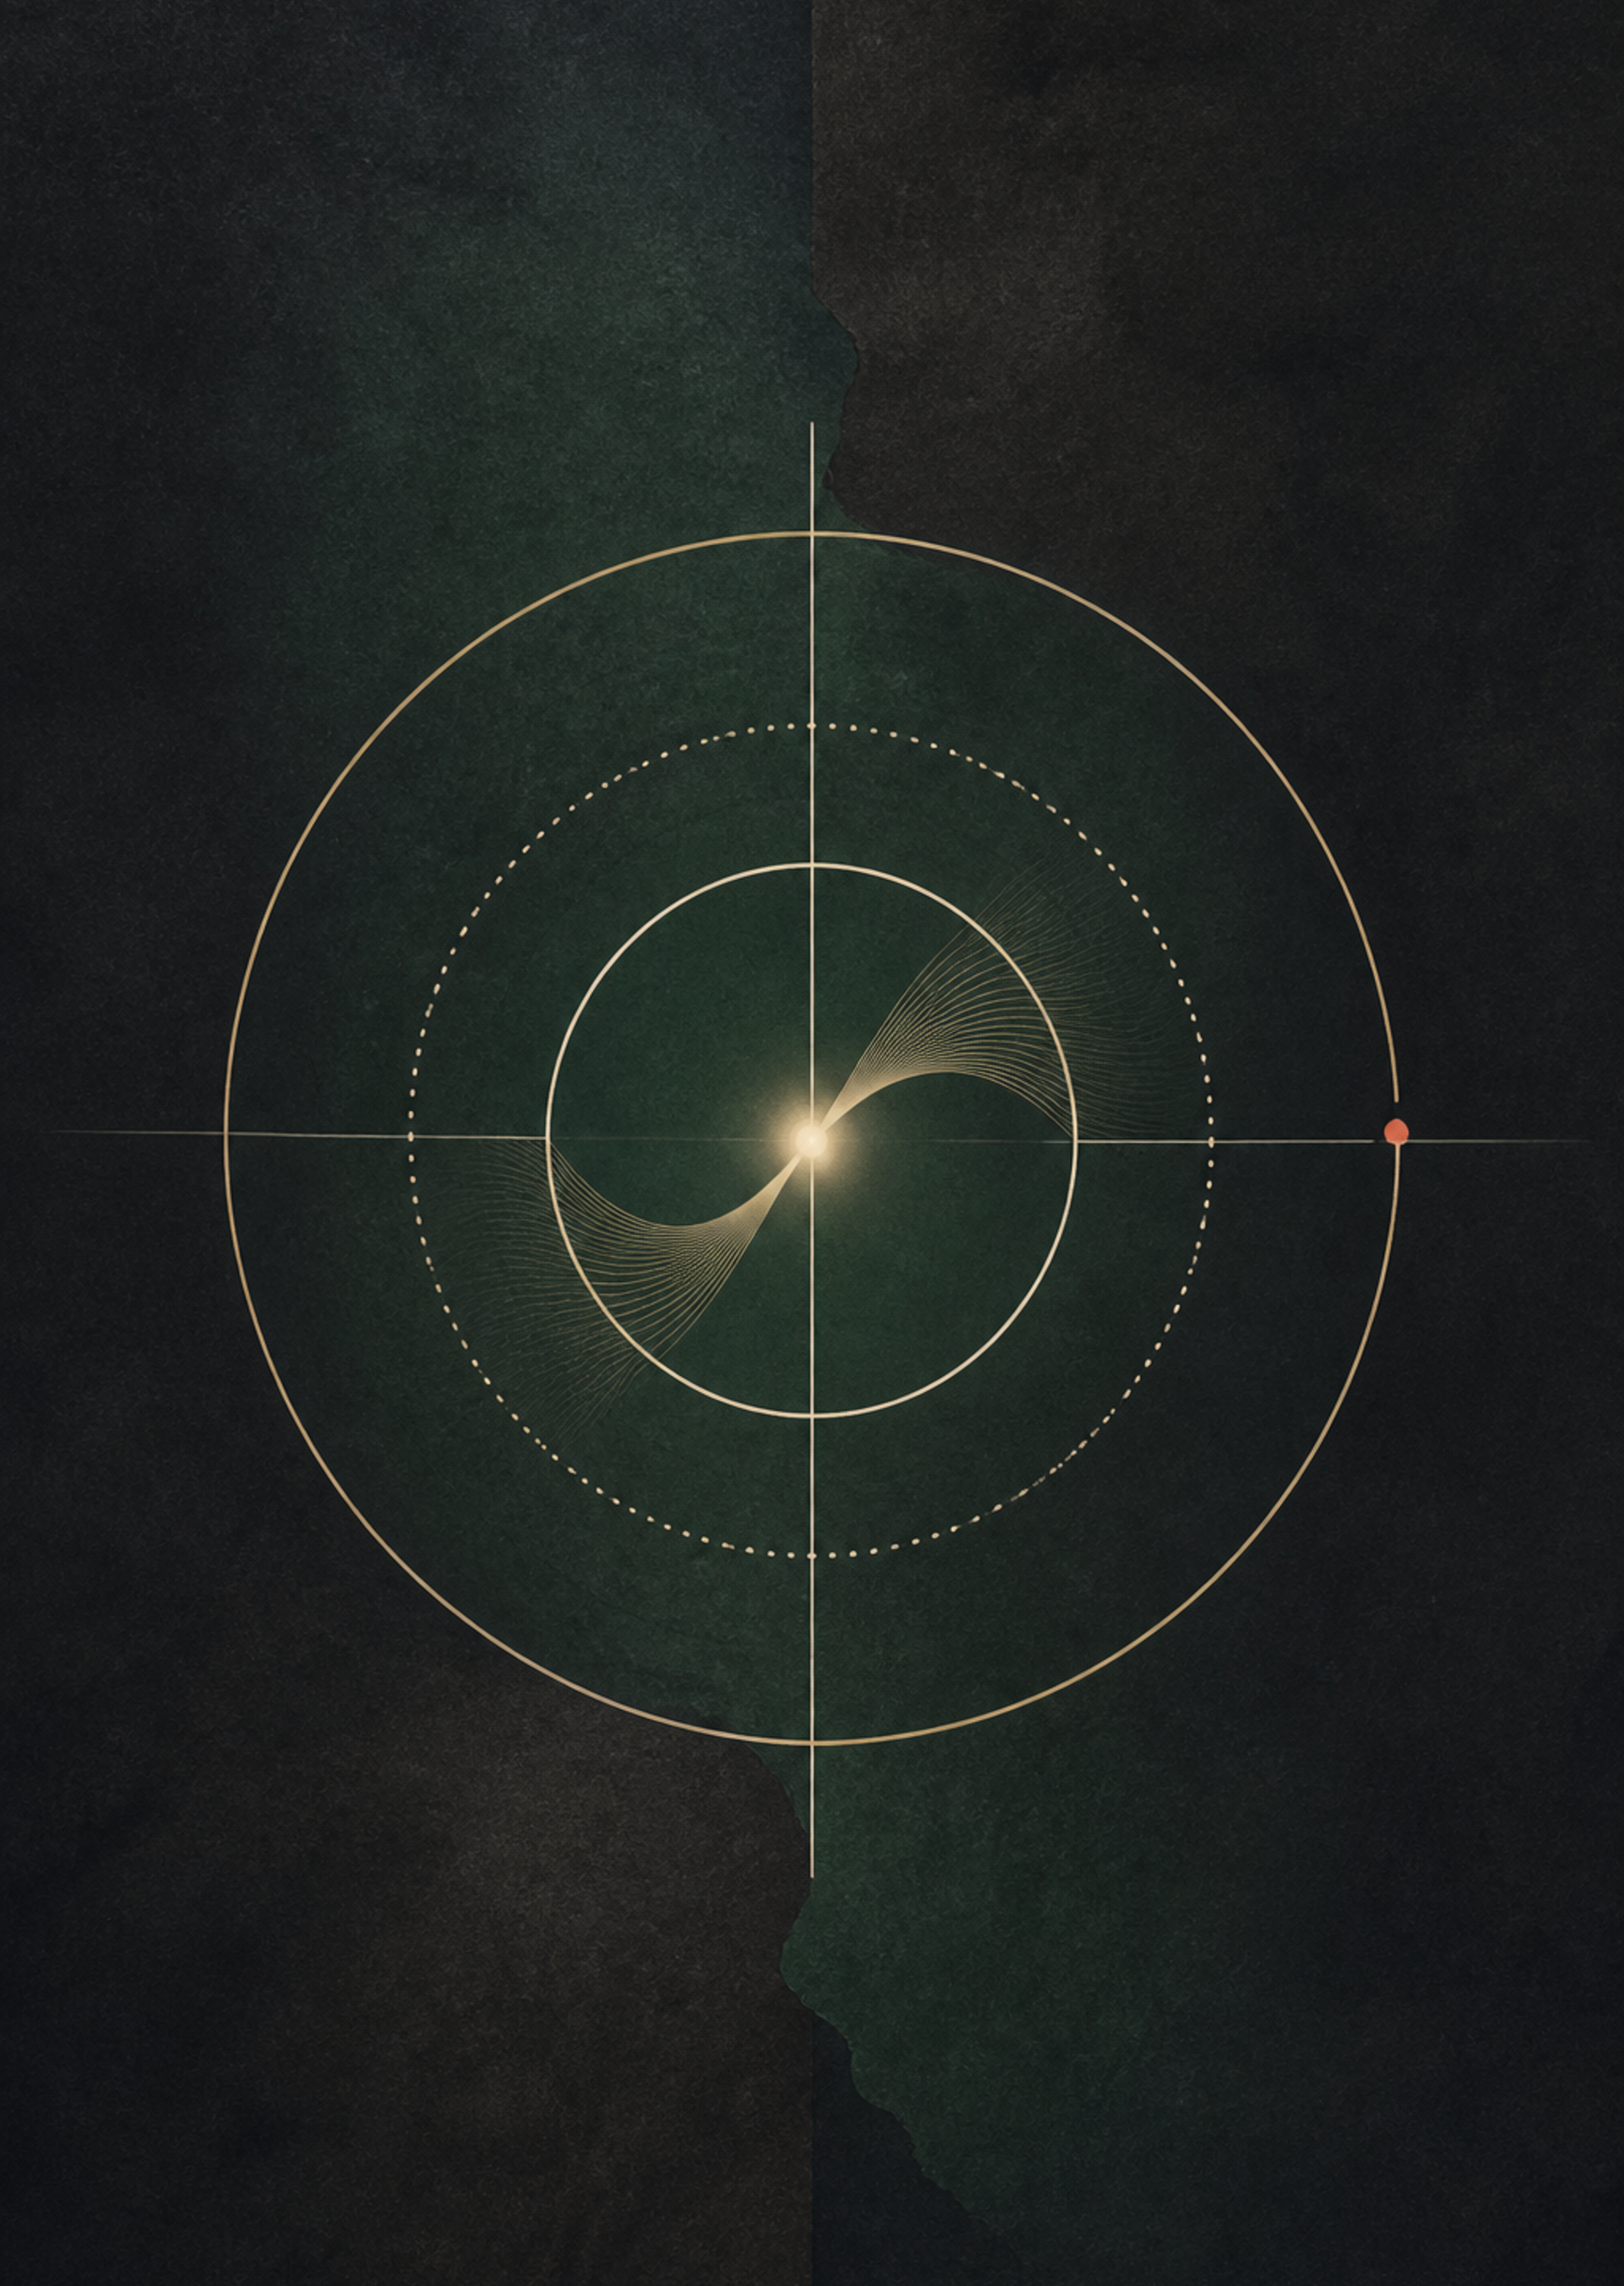
\includegraphics[height=\paperheight,keepaspectratio]{../../../generated_course_notes/supplementary/advanced_quantum_mechanics/2013_fall/assets/cover-art.png}%
  };
  \node[
    anchor=north west,
    align=left,
    text width=0.78\paperwidth,
    fill=white,
    fill opacity=0.9,
    rounded corners=8pt,
    inner xsep=10pt,
    inner ysep=8pt
  ] at ([xshift=0.08\paperwidth,yshift=-0.06\paperheight]current page.north west) {%
    {\fontsize{30}{33}\selectfont\bfseries\color{black!88} 量子力学特論\\[0.85em]}
    {\large\color{black!72} 日本語版 / 2013 fall}
  };
  \node[
    anchor=south west,
    align=left,
    text width=0.68\paperwidth,
    fill=white,
    fill opacity=0.82,
    text opacity=1,
    rounded corners=6pt,
    inner sep=12pt
  ] at ([xshift=0.08\paperwidth,yshift=0.08\paperheight]current page.south west) {%
    {\normalsize\color{black!78} 原講義：Leonard Susskind\\[0.35em]}
    {\small\color{black!72} 講義補助版：\href{https://lazying.art}{LazyingArt LLC} / \href{https://github.com/lachlanchen/Video2Book}{Video2Book}}
  };
\end{tikzpicture}
\mbox{}
\end{titlepage}
\hypersetup{pageanchor=true}

\clearpage
\chapter*{本ノートについて}
本書は、Leonard Susskindの講義に基づき、独立に編集された補助ノートである。機械による文字起こし、字幕、選定した黒板画像から内容を再構成し、利用可能な原資料と照合した。Susskind教授自身による原稿ではなく、同教授による査読や承認も受けていない。

本版は \href{https://lazying.art}{LazyingArt LLC} がオープンソースの \href{https://github.com/lachlanchen/Video2Book}{Video2Book} ワークフローを用いて作成した。機械文字起こしは別途利用可能であり、認識誤りを含む可能性がある。編集上の明確化および自明でない再構成は脚注で識別されている。
\clearpage
\tableofcontents
\mainmatter
\chapter{状態ベクトル、ユニタリ発展、並進対称性}
\providecommand{\ket}[1]{\left\lvert#1\right\rangle}
\providecommand{\bra}[1]{\left\langle#1\right\rvert}

2四半期の空白の後、量子力学の迅速な復習は有用である。それは四半期全体を占めることはできない。これから先の主題は、量子力学がもともと開発された問題への応用である。すなわち、原子、電子と関連粒子、そして光子である。

原子が最初に来る。電子が原子の一部であるのに、どうして原子が電子より先に来るのか。最初は水素原子の基本方程式を書くのに必要なだけの電子力学があればよい。電子に似た粒子のより詳細な研究は後で行うことができる。これらの応用を通じて、対称性は繰り返し現れる道具となる。すなわち、対称性が量子力学でどのように表現され、系について何を意味するかである。

\section{状態、観測量、直交性}

古典力学では、状態は位相空間の点で表される。量子力学では、状態は複素ベクトル空間のベクトルで表される。これは抽象的なベクトルであり、通常の三次元空間の矢印ではない。状態ベクトルは加算でき、複素数を掛けることができ、それらを含む空間は特定の有限次元を持つ必要はない。

ディラック記法では、状態ベクトルをケットとして書き、
\begin{equation}
\ket{\psi},
\end{equation}
それに対応するブラを関連付ける。
\begin{equation}
\bra{\psi}.
\end{equation}
ブラとケットはエルミート共役によって関係付けられる。ブラとケットを組み合わせると内積が得られ、
\begin{equation}
\langle\phi|\psi\rangle,
\end{equation}
これは一般に複素数である。

観測量とは測定できるものである。位置、運動量、エネルギー、またはその他の測定可能な量である。量子力学では、観測量は線形エルミート演算子\(A\)で表され、
\begin{equation}
A^\dagger=A.
\end{equation}
エルミート性は実数性の演算子版である。特に、エルミート演算子の固有値は実数である。

\(A\)の固有ベクトルは次を満たす。
\begin{equation}
A\ket{\alpha}=\alpha\ket{\alpha}.
\end{equation}
可能な固有値は\(A\)を測定したときの可能な結果である。例えば、観測量が\(1\)、\(3\)、または\(7\)のみを与え得るなら、これらの数がその固有値である。その固有ベクトルは、結果が統計的ではなく確定している状態である。状態\(\ket{\alpha}\)では、\(A\)を測定すると確実に\(\alpha\)が得られる。

内積は状態間の重要な論理関係を表す。\(\ket{\phi}\)と\(\ket{\psi}\)を確実に区別する測定があるとしよう。そのとき状態は直交する。
\begin{equation}
\langle\phi|\psi\rangle=0.
\end{equation}
直交性とは、状態が曖昧さなく物理的に区別可能であることを意味する。規格化された状態では、
\begin{equation}
\langle\psi|\psi\rangle=1.
\end{equation}

\section{位置表示における粒子}

まず、直線上を運動する粒子を考える。その位置\(x\)は観測量である。起こりうる各位置\(x_0\)に対して、位置測定が確実に\(x_0\)を与える状態\(\ket{x_0}\)が存在する。

異なる位置に対応する状態は区別可能であり、したがって直交する。
\begin{equation}
x\neq x'
\quad\Longrightarrow\quad
\langle x'|x\rangle=0.
\end{equation}
任意の状態\(\ket{\psi}\)に対して、その位置状態との重なりが波動関数を定義する。
\begin{equation}
\psi(x)=\langle x|\psi\rangle.
\end{equation}
これが状態ベクトルの位置表示である。

波動関数自体は確率ではない。それは正、負、虚数、または完全に複素数であり得る。位置確率密度は
\begin{equation}
P(x)=\psi^*(x)\psi(x)=|\psi(x)|^2.
\end{equation}
この積は確率密度がそうでなければならないように非負である。規格化された波動関数では、
\begin{equation}
\int_{-\infty}^{\infty}dx\,|\psi(x)|^2=1.
\end{equation}

位置表示では、位置演算子は掛け算として作用する。
\begin{equation}
(\hat x\psi)(x)=x\psi(x).
\end{equation}
その固有関数は一点に集中した理想化された関数である。それらはディラックのデルタ関数として形式的に記述される。すなわち、位置固有値を中心とする非常に狭いスパイクである。それらの正確な超関数的定義は現在の復習には必要ない。

三次元では、位置は三つの成分\(x\)、\(y\)、\(z\)を持ち、位置状態は三次元空間の点を表す。そのような二つの状態は、点が少なくとも一つの座標で異なるときはいつでも直交する。一次元の記法は通常保持され、対応する三次元への拡張は理解されているものとする。

\section{運動量と確定運動量状態}

位置の各成分に対して、対応する運動量の成分が存在する。位置表示では、\(x\)軸に沿った運動量演算子は
\begin{equation}
\hat p_x=-i\hbar\frac{d}{dx}.
\end{equation}
したがって、抽象的なエルミート演算子は波動関数への操作として具体的に見ることもできる。

確定運動量\(p_0\)を持つ状態は固有値方程式を満たす。
\begin{equation}
\hat p_x\psi_{p_0}(x)=p_0\psi_{p_0}(x).
\end{equation}
\(\hat p_x\)の微分形式を代入すると
\begin{equation}
-i\hbar\frac{d\psi_{p_0}(x)}{dx}
=p_0\psi_{p_0}(x).
\end{equation}
波動関数の導関数は波動関数自体に比例するので、解は指数関数の形をとる。
\begin{equation}
\psi_{p_0}(x)\propto
\exp\left(\frac{ip_0x}{\hbar}\right).
\end{equation}

\begin{classroomqa}
\lecturetimestamp{00:24:26}
\audiencequestion{この微分方程式は任意の波動関数に対して成り立つか。}
\lecturerresponse{いいえ。これは確定した運動量をもつ状態に対する固有値方程式である。ほとんどの波動関数はこれを満たさず、この方程式は運動量固有関数を選び出す。}
\end{classroomqa}

位置固有状態と運動量固有状態の区別は明確である。位置固有関数は一点に集中している。運動量固有関数は
\begin{equation}
\left|\exp\left(\frac{ip_0x}{\hbar}\right)\right|^2=1.
\end{equation}
をもつ。したがってその絶対値は直線全体にわたって一定である。この理想化された意味で、確定した運動量は位置の完全な不確定性を意味し、同様に確定した位置は運動量の完全な不確定性を意味する。これは位置--運動量不確定性関係の極端な形である。

\begin{classroomqa}
\lecturetimestamp{00:26:36}
\audiencequestion{運動量が\(p_0\)であると分かっているのに、なぜ依然として確率分布が存在するのか。}
\lecturerresponse{表示されている量は位置測定に関するものであり、別の運動量測定に関するものではない。運動量と位置は異なる観測量である。理想化された運動量固有状態に対して、位置振幅は直線全体にわたって一定の絶対値をもつ。運動量に対する振幅は運動量表示に属し、フーリエ変換によって位置の波動関数と関係づけられる。}
\end{classroomqa}

\begin{classroomqa}
\lecturetimestamp{00:28:02}
\audiencequestion{波動関数がディラックのデルタ関数であるとき、位置の確率はどのように見えるか。}
\lecturerresponse{それは指定された位置に集中している。この理想化されたスパイクは位置の確実性を表している。}
\end{classroomqa}

\editorialnote{厳密な位置固有状態と運動量固有状態は一般化された状態である。ディラックのデルタと平面波は、直線全体上の通常の二乗可積分な規格化された波動関数ではなく、デルタ関数の文字通りの二乗は通常の超関数ではない。上述の記述は、それらの理想化された局在と一定の絶対値に関するものである。}

波動関数は形式的には、\(x\)の各値に対して一つの成分をもつベクトルとみなすことができる。しかし、通常の有限の列ベクトルとは異なり、それは連続無限個の成分をもつ。

\begin{classroomqa}
\lecturetimestamp{00:28:53}
\audiencequestion{状態ベクトルは列ベクトルで表されるのか。}
\lecturerresponse{そのように表すこともできるが、\(x\)が連続的に多くの値をとるため、位置の波動関数を通常の列として書くのは厄介である。形式的には連続的な列ベクトルとみなすことができ、対応するブラは連続的な行ベクトルとみなされる。}
\end{classroomqa}

\section{時間発展とユニタリ性}

状態は時間とともにどのように変化するか。時間発展は状態の空間上の変換である。経過時間\(t\)にわたる発展を\(U(t)\)で表す。すると
\begin{equation}
U(t)\ket{\psi(t_1)}=\ket{\psi(t_1+t)}.
\end{equation}
特に、
\begin{equation}
\ket{\psi(t)}=U(t)\ket{\psi(0)},
\qquad
U(0)=\mathbf 1.
\end{equation}

\(U(t)\)に対する条件は情報の保存から従う。二つの初期状態が区別可能であるならば、時間発展はその区別を消してはならない。直交する状態は直交したままでなければならない。より一般に、任意の二つの状態の間の内積が保存される：
\begin{equation}
\langle U(t)\phi|U(t)\psi\rangle
=\langle\phi|\psi\rangle.
\end{equation}

\begin{equation}
\langle U(t)\phi|U(t)\psi\rangle
=\langle\phi|U^\dagger(t)U(t)|\psi\rangle,
\end{equation}
であるから、すべての内積の保存は
\begin{equation}
U^\dagger(t)U(t)=\mathbf 1.
\end{equation}
を要求する。この方程式を満たす演算子はユニタリである。

\begin{classroomqa}
\lecturetimestamp{00:36:36}
\audiencequestion{すべての内積を保存することは、単に直交性を保存することよりも強い主張か。}
\lecturerresponse{ここで議論している線形な状態変換については、直交性の保存は内積の保存に導く。通常の回転が身近な類推を与える：それらは直交性と内積を保存する。}
\end{classroomqa}

\editorialnote{厳密には、直交性の保存だけでは全体の非零の再スケーリングが許される。物理的な時間発展にすでに要求される規格化の保存がその自由度を除き、内積の保存を与える。}

ユニタリ演算子をエルミート観測量と混同してはならない。位置と運動量はエルミートであるが、一般にユニタリではない。ユニタリ演算子の固有値は位相であり、単位円上にある\(e^{i\theta}\)の形の数である。

\begin{classroomqa}
\lecturetimestamp{00:38:12}
\audiencequestion{非ユニタリ変換の例は何ですか。}
\lecturerresponse{位置演算子と運動量演算子がその例である。これらはエルミートな観測量であるが、ユニタリではない。ユニタリ演算子の固有値は絶対値が1であり、したがって位相因子である。}
\end{classroomqa}


\section{ハミルトニアンとSchr\"odinger方程式}

時間発展は連続であると仮定する。非常に短い区間 \(\epsilon\) の間では、発展演算子はしたがって恒等演算子に近くなければならない。
\begin{equation}
U(\epsilon)=\mathbf 1+\epsilon G+\mathcal O(\epsilon^2).
\end{equation}
ユニタリ性を用いると、
\begin{align}
U^\dagger(\epsilon)U(\epsilon)
&=
\left(\mathbf 1+\epsilon G^\dagger\right)
\left(\mathbf 1+\epsilon G\right)
+\mathcal O(\epsilon^2)
\\
&=
\mathbf 1+\epsilon(G^\dagger+G)
+\mathcal O(\epsilon^2).
\end{align}
一次まででは、
\begin{equation}
G^\dagger=-G.
\end{equation}
したがって \(G\) は反エルミートである。これは
\begin{equation}
G=-\frac{i}{\hbar}H,
\end{equation}
と書ける。ここで \(H\) はエルミートである。
\begin{equation}
H^\dagger=H.
\end{equation}
したがって無限小時間発展演算子は
\begin{equation}
U(\epsilon)
=
\mathbf 1-\frac{i\epsilon}{\hbar}H
+\mathcal O(\epsilon^2).
\end{equation}
である。エルミート演算子 \(H\) がハミルトニアンである。

\begin{classroomqa}
\lecturetimestamp{00:45:48}
\audiencequestion{何が \(\epsilon^2\) の項を無視することを可能にするのですか。}
\lecturerresponse{計算は \(\epsilon\) の一次まで一貫して行われている。二次の計算ならば、\(-\epsilon^2H^2/(2\hbar^2)\) に比例する項を含むすべての二次の項が必要であろう。近似は \(U(\epsilon)\) の打ち切られた表式にあり、\(H\) のエルミート性にあるのではない。}
\end{classroomqa}

有限の時間間隔は多くの小さな区間から構成できる。\(t\)を長さ\(t/N\)の\(N\)個のステップに分割する。無限小変換を繰り返すと
\begin{equation}
U(t)
=
\lim_{N\to\infty}
\left(
\mathbf 1-\frac{itH}{N\hbar}
\right)^N
=
\exp\left(-\frac{iHt}{\hbar}\right).
\end{equation}
が得られる。指数関数は無限小変換の有限版である。

次に状態を\(t\)から\(t+\epsilon\)へ発展させる。
\begin{align}
\ket{\psi(t+\epsilon)}
&=
U(\epsilon)\ket{\psi(t)}
\\
&=
\left(
\mathbf 1-\frac{i\epsilon}{\hbar}H
\right)\ket{\psi(t)}
+\mathcal O(\epsilon^2).
\end{align}
\(\ket{\psi(t)}\)を引き、\(\epsilon\)で割り、極限を取ると
\begin{equation}
\frac{d}{dt}\ket{\psi(t)}
=
-\frac{i}{\hbar}H\ket{\psi(t)}.
\end{equation}
が得られる。等価的に、
\begin{equation}
i\hbar\frac{d}{dt}\ket{\psi(t)}
=
H\ket{\psi(t)}.
\end{equation}
である。これが時間依存Schr\"odinger方程式である。位置表示では
\begin{equation}
i\hbar\frac{\partial}{\partial t}\psi(x,t)
=
H\psi(x,t),
\end{equation}
となる。ここで\(H\)は波動関数に作用する演算子として働く。

時間に依存しないSchr\"odinger方程式はハミルトニアンの固有値方程式である。
\begin{equation}
H\ket{E}=E\ket{E}.
\end{equation}
固有値\(E\)は測定されうるエネルギー、すなわちエネルギー準位である。したがって同じハミルトニアンが、許されるエネルギーと状態の発展の両方を決定する。

初期状態がエネルギー固有状態ならば、その発展は
\begin{equation}
\ket{E;t}
=
\exp\left(-\frac{iEt}{\hbar}\right)\ket{E}.
\end{equation}
である。それは同じエネルギー固有ベクトルのままであり、位相だけを得る。\footnote{負号は\(U(t)=\exp(-iHt/\hbar)\)の先行する導出によって固定される。後に口頭で述べられた位相の表式は反対の符号を持ち、その導出と矛盾する。}

\begin{classroomqa}
\lecturetimestamp{01:01:05}
\audiencequestion{エネルギー固有ベクトルは時間依存Schr\"odinger方程式の下でどのように発展するか。}
\lecturerresponse{ケットを保つ。\(H\ket{E}=E\ket{E}\)であるから、時間発展はエネルギー固有ベクトルにそのエネルギーで決まる位相を掛ける。\(\exp(-iEt/\hbar)\)。}
\end{classroomqa}

\section{何が対称性とみなされるか。}

時間発展は状態空間上の一つのユニタリ変換である。対称変換はもう一つの重要なクラスである。

回転対称性は原子物理学の中心である。水素原子では、電子は中心クーロンポテンシャル中を運動する。座標系を回転しても方程式は変わらず、物理的に原子を回転しても同じ方程式に支配される水素原子のままである。状態は回転の下で変化しうるが、力学法則は変化しない。

並進はもう一つの例を与える。空空間中の孤立系は、そのすべての部分が同じ量だけ変位した後でも同じように振る舞うはずである。この限定条件は重要である。炉が存在し、系だけが炉に近づけられるならば、系は異なる振る舞いをするかもしれない。炉はその並進対称性を破る。系と炉の両方が一緒に並進されるならば、それらの間の元の関係は回復される。

すべての操作が対称性であるわけではない。岩塩の結晶を半分に圧縮すると、一般にその振る舞いは変わる。圧縮は明確に定義された変換であるが、一般には対称性ではない。

したがって対称性とは、力学の形を保つ状態上の操作である。それを\(V\)で表す。それは識別可能性を保たなければならない。2つの直交状態は変換後も直交しなければならない。したがって、
\begin{equation}
V^\dagger V=\mathbf 1,
\end{equation}
であるから、\(V\)はユニタリである。

\section{対称性は時間発展と可換である}

初期状態\(\ket{\psi_1}\)が\(\ket{\psi_2}\)へ発展するとする。
\begin{equation}
\ket{\psi_2}=U(t)\ket{\psi_1}.
\end{equation}
提案された対称性\(V\)を両方の状態に適用する。
\begin{equation}
\ket{\psi_1'}=V\ket{\psi_1},
\qquad
\ket{\psi_2'}=V\ket{\psi_2}.
\end{equation}
\(V\)が力学の対称性ならば、変換された初期状態は変換された最終状態へ発展しなければならない。
\begin{equation}
\ket{\psi_2'}=U(t)\ket{\psi_1'}.
\end{equation}
定義を代入すると
\begin{equation}
VU(t)\ket{\psi_1}
=
U(t)V\ket{\psi_1}.
\end{equation}
が得られる。これはすべての初期状態について成り立たなければならない。したがって
\begin{equation}
VU(t)=U(t)V.
\end{equation}

二つの等価な経路は可換図式として表示できる。\footnote{この図式は01：10：30と01：16：34の間で展開された二経路の議論を再構成する。}
\begin{figure}
\centering
\begin{tikzpicture}[>=Stealth]
\node (a) at (0,0) {$\ket{\psi_1}$};
\node (b) at (4.2,0) {$\ket{\psi_2}=U(t)\ket{\psi_1}$};
\node (c) at (0,-2.0) {$V\ket{\psi_1}$};
\node (d) at (4.2,-2.0) {$V\ket{\psi_2}=U(t)V\ket{\psi_1}$};

\draw[->] (a) -- node[above] {$U(t)$} (b);
\draw[->] (c) -- node[below] {$U(t)$} (d);
\draw[->] (a) -- node[left] {$V$} (c);
\draw[->] (b) -- node[right] {$V$} (d);
\end{tikzpicture}
\caption{対称操作と時間発展は、どちらの順序でも同じ最終状態を与える。}
\end{figure}

\begin{classroomqa}
\lecturetimestamp{01:16:38}
\audiencequestion{対称性はすべての時間について時間発展と可換でなければならないか？}
\lecturerresponse{はい。力学の対称性は、全時間発展に対して可換条件を満たさなければならない。}
\end{classroomqa}

\begin{classroomqa}
\lecturetimestamp{01:17:13}
\audiencequestion{これは、回転してから待ってもよいし、待ってから回転してもよいという意味か？}
\lecturerresponse{そのとおり。回転が対称性ならば、どちらの順序でも同じ変換された最終状態が得られる。}
\end{classroomqa}

小さな時間間隔に対して、
\begin{equation}
U(\epsilon)
=
\mathbf 1-\frac{i\epsilon}{\hbar}H
+\mathcal O(\epsilon^2).
\end{equation}
可換条件は
\begin{equation}
V\left(
\mathbf 1-\frac{i\epsilon}{\hbar}H
\right)
=
\left(
\mathbf 1-\frac{i\epsilon}{\hbar}H
\right)V
+\mathcal O(\epsilon^2).
\end{equation}
となる。恒等項は相殺し、
\begin{equation}
VH=HV,
\end{equation}
または
\begin{equation}
[V,H]=0.
\end{equation}
が残る。したがって、ユニタリ操作が力学の対称性であるのは、それがハミルトニアンと可換であるまさにそのときに限る。

\begin{classroomqa}
\lecturetimestamp{01:19:29}
\audiencequestion{対称操作\(V\)がユニタリであることを要求するものは何か？}
\lecturerresponse{対称性は状態間の論理的区別を保存しなければならない。互いに排他的な直交状態を、もはや区別できない状態に移してはならない。それらの関係を保存することはユニタリ変換を要求する。}
\end{classroomqa}

明示的な時間依存を持たず\(H\)と可換な演算子は保存される。これは対称性と保存則を結びつける。古典力学では、この関係はネーターの定理によって表される。現在の量子力学的な形では、中心となる判定基準はハミルトニアンとの交換子である。

\section{離散対称性と連続対称性}

対称性は離散的または連続的でありうる。鏡映は離散的である。それは左と右を交換し、両者の間に無限小の鏡映の列は存在しない。二つの同一粒子を交換することは別の離散的操作である。印のない両面物体を裏返すことも同種の例を与える。

回転は連続的である。\(90^\circ\)の回転は、同じ軸のまわりの多くの小さな回転から構成できる。空間並進も同じ理由で連続的である。有限の変位は、多くの微小変位から構成できる。

この小さな変換への分割可能性が、連続対称性に特別な形を与える。恒等変換の近くで、
\begin{equation}
V(\epsilon)
=
\mathbf 1-i\epsilon G+\mathcal O(\epsilon^2),
\end{equation}
と書く。ここで\(\epsilon\)は変換をパラメータ化する。ユニタリ性は
\begin{equation}
G^\dagger=G.
\end{equation}
を意味する。エルミート演算子\(G\)は対称性の生成子と呼ばれる。

変換が対称性ならば、
\begin{equation}
[H,V(\epsilon)]=0.
\end{equation}
である。一次まで展開すると
\begin{equation}
[H,G]=0.
\end{equation}
が得られる。したがって、連続対称性はハミルトニアンと可換なエルミート演算子によって生成される。それらの生成子は保存量である。

``生成される''という語は、ここでは具体的な意味を持つ。有限変換は、有限の時間発展が多くの短い時間ステップから構成されるのとちょうど同じように、無限小変換を繰り返し適用することによって構成される。

\section{並進対称性と運動量}

波動関数を距離\(\epsilon\)だけ右へ能動的に平行移動することを考えよう。もとの波動関数が\(x_0\)にピークをもつなら、平行移動後の波動関数は\(x_0+\epsilon\)にピークをもつはずである。したがって座標\(x\)におけるその値は、\(x-\epsilon\)で評価したもとの波動関数である：
\begin{equation}
(T(\epsilon)\psi)(x)=\psi(x-\epsilon).
\end{equation}
微小変位に対しては、
\begin{equation}
\psi(x-\epsilon)
=
\psi(x)-\epsilon\frac{d\psi(x)}{dx}
+\mathcal O(\epsilon^2).
\end{equation}
したがって
\begin{equation}
T(\epsilon)
=
\mathbf 1-\epsilon\frac{d}{dx}
+\mathcal O(\epsilon^2).
\end{equation}
\begin{equation}
\hat p_x=-i\hbar\frac{d}{dx},
\qquad
\frac{d}{dx}=\frac{i}{\hbar}\hat p_x,
\end{equation}
を用いると、無限小平行移動は
\begin{equation}
T(\epsilon)
=
\mathbf 1-\frac{i\epsilon}{\hbar}\hat p_x
+\mathcal O(\epsilon^2).
\end{equation}
となる。対応する有限平行移動は
\begin{equation}
T(\epsilon)
=
\exp\left(-\frac{i\epsilon}{\hbar}\hat p_x\right).
\end{equation}
である。規約\(V(\epsilon)=\mathbf 1-i\epsilon G+\cdots\)のもとでは、次元をもつ平行移動パラメータにより
\begin{equation}
G_{\mathrm{trans}}=\frac{\hat p_x}{\hbar}.
\end{equation}
が得られる。同値な言い方をすれば、指数の中に\(\hbar\)の因子が現れるとき、運動量は空間平行移動の生成子と呼ばれる。

\begin{classroomqa}
\lecturetimestamp{01:34:08}
\audiencequestion{並進の導出で負符号が失われていないか？}
\lecturerresponse{問題は、並進された波動関数に割り当てられる向きである。右への能動的シフトは\(\psi(x+\epsilon)\)ではなく\(\psi(x-\epsilon)\)で表される。その修正により、\(T(\epsilon)=\mathbf 1-i\epsilon\hat p_x/\hbar+\cdots\)。}
\end{classroomqa}

運動量が保存されるかどうかはハミルトニアンに依存する。一次元を運動する自由粒子に対して、
\begin{equation}
H=\frac{\hat p_x^2}{2m}.
\end{equation}
すべての演算子はそれ自身の任意の関数と可換であるから、
\begin{equation}
[H,\hat p_x]=0.
\end{equation}
したがって自由粒子ハミルトニアンは並進の下で不変であり、\(\hat p_x\)は保存される。物理的には、粒子は初期位置をどこに選んでも同じように振る舞う。初期条件を並進させることは、運動全体を並進させるだけである。

三次元では、
\begin{equation}
H
=
\frac{\hat p_x^2+\hat p_y^2+\hat p_z^2}{2m}.
\end{equation}
各運動量成分は\(H\)と可換である：
\begin{equation}
[H,\hat p_x]=[H,\hat p_y]=[H,\hat p_z]=0.
\end{equation}
各空間方向に独立な並進対称性が存在する。運動量は保存量であると同時に、それらの並進に対応する生成子でもある。

次の場合は回転対称性である。異なる軸のまわりの回転は一般に可換でないため、回転はより込み入っている。すなわち、\(x\)回転に続く\(y\)回転は、逆の順序と同じではない。このことが、非可換な対称性の生成子と、回転の群論的構造をもたらす。

\chapter{対称性、縮退、角運動量のはしご}
\providecommand{\ket}[1]{\left\lvert#1\right\rangle}

\section{対称性と縮退したエネルギー準位}

対称性とは、系の物理的記述を変えない操作である。それはハミルトニアン、Schr\"odinger方程式、あるいは取り得るエネルギーを変えない。ユニタリ演算子\(S\)がその操作を表すならば、不変性とは
\begin{equation}
S H S^\dagger=H,
\end{equation}
を意味し、あるいは等価的に
\begin{equation}
[S,H]=0.
\end{equation}
である。

並進はその一例である。原子を一つの場所から別の場所へ移しても、そのエネルギーは変わらない。これは基底状態だけでなく、すべての原子状態について成り立つ。回転もまた一例であり、ここでの主要な主題となる。

二つの同一粒子を入れ替えることもまた対称性である。二つの電子を電子1と電子2、あるいはハリーとフレッドと呼んでも、それらが異なるものになるわけではない。ラベルを入れ替えても原子の性質は変わり得ない。

結晶にはさらに別種の並進対称性がある。結晶全体を空間中で動かすのは通常の並進である。しかし無限結晶に対しては、一格子間隔だけ並進させても同じ物理的配置が得られる。等価的に、すべての格子点の指数を1だけずらすことによって格子点を付け替えることができる。境界は有限結晶に対してこの厳密な主張を損なうが、非常に長い結晶の端から遠く離れたところでは良い対称性となる。

空間の一様性---すべての位置が他のすべての位置と同じであるという事実---は並進対称性である。空間の等方性---すべての方向が他のすべての方向と同じであるという事実---は回転対称性である。

縮退は対称性と関係しているが、同じものではない。あるエネルギー準位は、複数の状態がちょうどそのエネルギーをもつとき縮退しているという。離散スペクトルをもつ一般的なハミルトニアンに対して、無関係な二つの準位の間の厳密な等しさは驚くべき偶然であろう。\(10^{15}\)分の1までの一致であっても、依然として厳密な等しさではない。厳密な縮退は通常、対称性を指し示す。

対称性はときに縮退を意味するが、常にそうではない。最初の例は、なぜそうなり得るのか、そしてなぜ一つの対称性だけでは不十分であり得るのかの両方を示す。

\section{円周上の粒子}

円形の針金の上を運動するよう拘束されたビーズを考える。その位置はデカルト座標\(x\)と\(y\)で記述することもできるが、一つの角度座標で十分である：
\begin{equation}
\psi=\psi(\theta).
\end{equation}
円周上の位置確率密度は\(\psi^*(\theta)\psi(\theta)\)である。

小さな角度\(\epsilon\)だけ反時計回りに能動的に回転させると、
\begin{equation}
\psi(\theta)\longrightarrow\psi(\theta-\epsilon).
\end{equation}
したがって
\begin{align}
\delta\psi(\theta)
&=\psi(\theta-\epsilon)-\psi(\theta)\\
&=-\epsilon\frac{d\psi}{d\theta}
+\mathcal O(\epsilon^2).
\end{align}

演算子
\begin{equation}
L_z=-i\hbar\frac{d}{d\theta}
\end{equation}
は周期的な波動関数上でエルミートである。これは
\begin{equation}
p_x=-i\hbar\frac{d}{dx}.
\end{equation}
の角度版である。\(i\)の因子はエルミート性にとって不可欠である。\(L_z\)を用いると、
\begin{equation}
\delta\psi
=-\frac{i\epsilon}{\hbar}L_z\psi
+\mathcal O(\epsilon^2),
\end{equation}
であるから、無限小回転演算子は
\begin{equation}
R(\epsilon)
=1-\frac{i\epsilon}{\hbar}L_z
+\mathcal O(\epsilon^2).
\end{equation}
となる。これにより\(L_z\)が円周に垂直な軸のまわりの回転の生成子であることが同定される。

\begin{classroomqa}
\lecturetimestamp{00:11:19}
\audiencequestion{\(i\)を含む因子の一方は逆符号であるべきではないか？}
\lecturerresponse{符号を確認すると上の関係が得られる。規約\(\psi(\theta)\to\psi(\theta-\epsilon)\)では、変化は\(-\epsilon\,d\psi/d\theta\)であり、これは\(-i\epsilon L_z\psi/\hbar\)に等しい。}
\end{classroomqa}

次に角運動量の固有状態を求める：
\begin{equation}
L_z\psi=M\psi.
\end{equation}
微分演算子を代入すると
\begin{equation}
-i\hbar\frac{d\psi}{d\theta}=M\psi,
\end{equation}
が得られ、その解は
\begin{equation}
\psi(\theta)=C\exp\left(\frac{iM\theta}{\hbar}\right).
\end{equation}
の形をとる。

無限直線上の運動には現れない追加の条件がある。点\(\theta=0\)と\(\theta=2\pi\)は同じ点であるから、一価の軌道波動関数は
\begin{equation}
\psi(\theta+2\pi)=\psi(\theta).
\end{equation}
を満たさなければならない。上の固有関数に対して、これは
\begin{equation}
\exp\left(\frac{2\pi iM}{\hbar}\right)=1.
\end{equation}
を要求する。したがって、
\begin{equation}
M=m\hbar,
\qquad
m\in\mathbb Z.
\end{equation}
円周上で可能な軌道角運動量はしたがって
\begin{equation}
\ldots,-2\hbar,-\hbar,0,\hbar,2\hbar,\ldots.
\end{equation}
である。

角運動量\(m\hbar\)をもつ状態は、角運動量\(-m\hbar\)をもつ状態と同じエネルギーをもたなければならないのだろうか？正と負の\(m\)は反対向きの循環を記述する。問題は、回転対称性だけがそれら二つの運動に等しいエネルギーを要求するかどうかである。

\begin{classroomqa}
\lecturetimestamp{00:22:51}
\audiencequestion{\(\psi(\theta-\epsilon)\)を用いることは、粒子が時計回りに運動していることを意味するのか？}
\lecturerresponse{いいえ。その規約はどの方向を正の回転と呼ぶかを定めるだけである。それは角度位置と角運動量の符号を定義するが、粒子が実際に運動する方向を決定するものではない。}
\end{classroomqa}

円周の面に垂直な磁場が反例を与える。それは正と負の角運動量のエネルギーを反対方向にずらし、それによってその対を分裂させ得る。ずれの符号は電荷と配向の規約に依存するが、分裂が重要な点である。

そのような場は依然として垂直軸のまわりの回転を保存する。したがって、回転対称性それ自体は
\begin{equation}
E(m)=E(-m).
\end{equation}
を要求しないことを示している。分裂がなければ、\(m=1\) と \(m=-1\) は縮退した対をなし得るし、\(m=2\) と \(m=-2\) も同様であり得る。状態 \(m=0\) には、この種の異なる相手が存在しない。

\section{反射対称性と \texorpdfstring{\(m,-m\)}{m, -m} 対}

離散的な反射対称性を加える。\(\mathcal M\) を円の直径に関する反射を表すものとする：
\begin{equation}
(\mathcal M\psi)(\theta)=\psi(-\theta).
\end{equation}
それは循環の向きを逆にする：
\begin{equation}
\mathcal M\psi_m=\psi_{-m}.
\end{equation}

反射が対称性ならば、
\begin{equation}
[\mathcal M,H]=0.
\end{equation}
である。
\begin{equation}
H\ket{m}=E_m\ket{m}.
\end{equation}
と仮定する。\(\mathcal M\) を適用すると
\begin{align}
H\mathcal M\ket{m}
&=\mathcal M H\ket{m}\\
&=E_m\mathcal M\ket{m}.
\end{align}
が得られる。\(\mathcal M\ket{m}\) は角運動量 \(-m\hbar\) をもつ状態であるから、
\begin{equation}
E_{-m}=E_m.
\end{equation}
である。回転対称性は角運動量を保存し、反射対称性は二つの反対の値を関係づける。両者を合わせると、その対が縮退していることが要求される。

\begin{classroomqa}
\lecturetimestamp{00:29:54}
\audiencequestion{\(m\) モードと \(-m\) モードは同じ確率密度をもつので、それだけでそれらのエネルギーが等しいことが示されるのか？}
\lecturerresponse{いいえ。波動関数 \(e^{im\theta}\) と \(e^{-im\theta}\) は、その絶対値の二乗が一致していても異なる。角運動量固有値方程式は波動関数を関与させ、\(\psi^*\psi\) だけではない。量子力学は確率だけでなく振幅を要求する。}
\end{classroomqa}

磁場はその軸のまわりの回転を保存するが、上で用いた反射を破る。

\begin{classroomqa}
\lecturetimestamp{00:33:05}
\audiencequestion{反射対称性は磁場を逆にするのか？}
\lecturerresponse{はい。磁場は軸性ベクトルである。板に垂直に入る向きの場を反射すると、板から出る向きの場が得られる。等価に、電流ループとその鏡像は逆向きの電流を運び、逆向きの場を生じる。}
\end{classroomqa}

回転と反射の非可換性は直接に見ることができる。角運動量固有関数に対して、
\begin{align}
\mathcal M L_z\psi_m
&=m\hbar\,\psi_{-m},\\
L_z\mathcal M\psi_m
&=-m\hbar\,\psi_{-m}.
\end{align}
したがって
\begin{equation}
[\mathcal M,L_z]\psi_m
=2m\hbar\,\psi_{-m},
\end{equation}
であり、これは \(m\neq0\) に対して非零である。回転してから反射する操作は、反射してから回転する操作と同じではない。

両方の変換が対称性であるとき、両方の演算子は \(H\) と可換であるが、互いに可換ではない。これが縮退の原因となるパターンである。

\begin{classroomqa}
\lecturetimestamp{00:40:28}
\audiencequestion{\(x\) と \(p\) のような非可換なハイゼンベルク対は縮退を生じるのか？}
\lecturerresponse{一般にはそうではない。演算子はまた対称性でなければならない：それらはハミルトニアンと可換でなければならない。位置と運動量は通常、両方が保存されるわけではない。もし両方が \(H\) と可換ならば、それらの非可換性は縮退を意味するであろう。}
\end{classroomqa}

\section{対称性の交換子代数}

\(A\) と \(B\) が二つの連続対称性のエルミート生成子であるとする：
\begin{equation}
[A,H]=0,
\qquad
[B,H]=0.
\end{equation}
これらの方程式のどこにも、\(A\) と \(B\) が互いに可換であることは要求されていない。

交換子 \([A,B]\) は反エルミートであるから、エルミート演算子
\begin{equation}
C=i[A,B].
\end{equation}
を定義する。数因子と全体の符号はここでは重要でない。重要な点は、\(C\) もまたハミルトニアンと可換であることである。実際、
\begin{equation}
[AB,H]
=A[B,H]+[A,H]B=0,
\end{equation}
であり、同様に
\begin{equation}
[BA,H]=0.
\end{equation}
である。したがって
\begin{equation}
[C,H]
=i\bigl([AB,H]-[BA,H]\bigr)=0.
\end{equation}

新しい生成子 \(C\) は \(A\) と \(B\) から独立であり得るし、すでに知られている生成子の線形結合にすぎないこともあり得る。もし新しいならば、それをリストに加えてさらなる交換子を作る。この過程を繰り返すと無限に続くこともあるが、しばしば有限個の生成子で閉じる：それ以上の交換子はすべて、すでに存在するものの線形結合である。その閉じた系が交換子代数またはリー代数である。

有限の対称変換は群をなす。それらの無限小生成子は対応するリー代数をなす。

縮退が重要であるのは、それがスペクトルを組織するからである。二つの状態が等しいエネルギーをもつならば、一方がそのエネルギー差を運ぶ光子を放出して他方へ崩壊することはできない。原子分光学では、準位の配置と縮退が可能なスペクトル線を決定する。同じ論理が励起ハドロンとその遷移にも当てはまる。

\begin{classroomqa}
\lecturetimestamp{00:49:07}
\audiencequestion{これらの交換子自体は対称群の要素なのか？}
\lecturerresponse{ここで議論している演算子は生成子である。生成子とそれらの交換子は交換子代数、すなわちリー代数をなす。生成子から作られる有限の対称操作が群の要素である。}
\end{classroomqa}

すべての対称性生成子が互いに可換ならば、その対称性は可換であると呼ばれる。それらの交換子のいくつかが非零ならば、非可換である。

\begin{classroomqa}
\lecturetimestamp{00:50:25}
\audiencequestion{生成子の基本的な定義とは何か。}
\lecturerresponse{恒等変換に非常に近いユニタリ対称変換をとり、それを\(1-i\epsilon G/\hbar+\cdots\)と書く。エルミート演算子\(G\)がその生成子である。対応する無限小変換を繰り返せば有限変換が構成される。}
\end{classroomqa}

\begin{classroomqa}
\lecturetimestamp{00:52:08}
\audiencequestion{対称性の生成子の代数とは何を意味するのか。}
\lecturerresponse{それは、加算、減算、通常の数による乗算、および交換ができる生成子の集合である。この代数では交換子が乗算の役割を果たし、閉性とはこれらの演算が集合の外の生成子を生じないことを意味する。}
\end{classroomqa}

\section{異なる軸のまわりの回転}

回転は非可換対称性の最も重要な例を与える。\(x\)軸のまわりの回転に続いて\(y\)軸のまわりの回転を行っても、一般には逆の順序で行った場合と同じにはならない。それらの不一致自体が第三の軸のまわりの回転と関係している。

\begin{classroomqa}
\lecturetimestamp{00:54:22}
\audiencequestion{有限回転は可換でないのに、無限小回転は可換なのか。}
\lecturerresponse{それらは二つの小さな回転角について二次の差がある。それで十分である。すなわち、それらの小さなパラメータをくくり出した後、生成子自身が非零の交換子をもつ。}
\end{classroomqa}

量子交換子を計算する前に、対応する古典的描像を考える。角運動量がその平面に垂直な円形の惑星軌道をとる。軌道全体を\(y\)軸のまわりに回転させると、全く同じエネルギーをもつ別の許された軌道が得られる。しかしその角運動量ベクトルは今や異なる\(x\)成分をもつ。

したがって回転不変性は、異なる角運動量成分をもつ同じエネルギーの配置を生み出す。量子力学的には、これは異なる軸のまわりの回転の生成子の間の非可換性として現れる。

\section{デカルト座標における角運動量}

まず、粒子を円周上に制限することなく、\(xy\)平面内を運動するものとして考える。微小な反時計回りの回転の下で、
\begin{equation}
\delta x=-\epsilon y,
\qquad
\delta y=\epsilon x.
\end{equation}
能動的に回転させた状態に対して、変換された波動関数は逆回転した座標で評価される：
\begin{equation}
\psi_\epsilon(x,y)
=\psi(x+\epsilon y,y-\epsilon x).
\end{equation}
したがって、
\begin{align}
\delta\psi
&=\epsilon\left(
y\frac{\partial}{\partial x}
-x\frac{\partial}{\partial y}
\right)\psi
+\mathcal O(\epsilon^2)\\
&=-\frac{i\epsilon}{\hbar}
\left(xp_y-yp_x\right)\psi
+\mathcal O(\epsilon^2).
\end{align}
よって、\(z\)軸のまわりの回転の生成子は
\begin{equation}
L_z=xp_y-yp_x.
\end{equation}
である。これは、よく知られた古典的ベクトル
\begin{equation}
\mathbf L=\mathbf r\times\mathbf p.
\end{equation}
の\(z\)成分である。それは力学的角運動量だけではなく、量子力学においては波動関数の回転を生成する演算子である。\footnote{能動的回転の規約は、先の変換\(\psi(\theta)\mapsto\psi(\theta-\epsilon)\)および、口頭での導出における途中の符号の不確定性の後の最終的な同定\(L_z=xp_y-yp_x\)と一致するように選ばれている。}

\(x\to y\to z\to x\)を巡回させると他の成分が得られる。\footnote{\(L_x\)および\(L_y\)の式は、講義で明示的に規定された巡回置換\(x\to y\to z\to x\)を\(L_z=xp_y-yp_x\)に適用することによって再構成される。}
\begin{align}
L_x&=yp_z-zp_y,\\
L_y&=zp_x-xp_z,\\
L_z&=xp_y-yp_x.
\end{align}

回転不変な系に対して、これらの演算子はハミルトニアンと交換する。
\begin{equation}
[H,L_x]=[H,L_y]=[H,L_z]=0.
\end{equation}
中心力場中の粒子が標準的な例である。これらの式は量子形式における角運動量保存である。

\section{角運動量リー代数}

正準交換関係は
\begin{align}
[x_i,x_j]&=0,\\
[p_i,p_j]&=0,\\
[x_i,p_j]&=i\hbar\,\delta_{ij}.
\end{align}
座標は異なる方向に属する運動量成分と交換する。したがって例えば\(x\)は\(p_y\)と交換するが、\(x\)は\(p_x\)と交換しない。

次に
\begin{equation}
[L_x,L_y]
=
[yp_z-zp_y,\;zp_x-xp_z].
\end{equation}
を計算する。ほとんどの項は消える。非零の二つの寄与は
\begin{align}
[yp_z,zp_x]&=-i\hbar\,yp_x,\\
[zp_y,xp_z]&=i\hbar\,xp_y.
\end{align}
である。したがって
\begin{align}
[L_x,L_y]
&=i\hbar\left(xp_y-yp_x\right)\\
&=i\hbar L_z.
\end{align}
座標ラベルを巡回させると
\begin{align}
[L_x,L_y]&=i\hbar L_z,\\
[L_y,L_z]&=i\hbar L_x,\\
[L_z,L_x]&=i\hbar L_y.
\end{align}

\begin{classroomqa}
\lecturetimestamp{01:14:50}
\audiencequestion{交換子が\(L_z\)を生み出すとき、\(L_z\)が\(L_x\)と\(L_y\)の線形結合でないことを依然として示さなければならないのか。}
\lecturerresponse{はい。その独立性を仮定するのではなく確立する義務がある。この時点では直接的な代数的証明は行わない。}
\end{classroomqa}

表示された交換子は\(L_x\)、\(L_y\)、\(L_z\)の張る空間上で閉じている。すなわち、これら三つをすべて含めれば、それ以上の交換子はその空間の外の演算子を生じない。これが角運動量リー代数である。
\begin{equation}
[H,L_i]=0,
\qquad i=x,y,z,
\end{equation}
と合わせて、これらの関係は、角Schr\"odinger方程式を直接解くことを要せずに、エネルギー準位についての相当な情報を含んでいる。

同様の代数的戦略は量子調和振動子にも用いられ、そこでは生成演算子と消滅演算子がそのスペクトルを生成する。ここでは、類似の演算子はエネルギーではなく角運動量の \(z\) 成分を変化させる。

\(z\) 軸を選ぶことは表現の選択にすぎない。\(z\) が \(x\) や \(y\) より物理的に好ましいわけではないが、一つの成分を選ぶと便利な基底が得られる。
\begin{equation}
L_z\ket{m}=m\hbar\ket{m}.
\end{equation}
課題は、\(m\) のどの値が起こり得るか、そして異なる \(m\) をもつ状態がどのように関係するかを決定することである。

\begin{classroomqa}
\lecturetimestamp{01:24:02}
\audiencequestion{この構成を調和振動子と比較するというのは、量子調和振動子のことですか。それは前回の授業では扱われませんでした。}
\lecturerresponse{はい、比較は量子振動子との比較である。現在の角運動量の議論は自己完結しており、振動子の知識を必要としない。この類推は後に逆方向にも読める：振動子は同様の代数学的方法を用いる。}
\end{classroomqa}

\section{角運動量の昇降}

定義する
\begin{equation}
L_+=L_x+iL_y,
\qquad
L_-=L_x-iL_y.
\end{equation}
角運動量の交換関係は次を意味する
\begin{equation}
[L_z,L_+]=\hbar L_+,
\qquad
[L_z,L_-]=-\hbar L_-.
\end{equation}

最初の関係を \(L_z\) の固有状態に適用する：
\begin{align}
L_zL_+\ket{m}
&=\left(L_+L_z+[L_z,L_+]\right)\ket{m}\\
&=(m+1)\hbar\,L_+\ket{m}.
\end{align}
\(L_+\ket{m}=0\) でない限り、それは \(L_z\) の別の固有状態であり、今度は固有値 \((m+1)\hbar\) をもつ。同様に、
\begin{equation}
L_zL_-\ket{m}
=(m-1)\hbar\,L_-\ket{m}.
\end{equation}
したがって \(L_+\) は \(m\) を 1 だけ上げ、\(L_-\) はそれを 1 だけ下げる。

任意の一つの固有値から出発して、代数は整数で隔てられた列を生成する。その列は無限に続くこともあれば、上端で
\begin{equation}
L_+\ket{m_{\mathrm{top}}}=0
\end{equation}
下端で
\begin{equation}
L_-\ket{m_{\mathrm{bottom}}}=0
\end{equation}
となるために終わることもある。

\begin{classroomqa}
\lecturetimestamp{01:35:11}
\audiencequestion{角運動量は円の議論によってすでに整数であることが要求されていたのではないですか。}
\lecturerresponse{その議論は、一価の位置波動関数で表される軌道角運動量に対して整数値を証明する。抽象的な角運動量代数はより緩い結果を与える：はしごは整数値または半整数値のいずれかを含み得る。}
\end{classroomqa}

はしごに端がある場合、回転不変性によってその両端が関係づけられる。\(z\)に垂直な軸のまわりに\(180^\circ\)回転すると、次の変換が生じる。
\begin{equation}
L_z\longrightarrow-L_z.
\end{equation}
したがって、スペクトルはゼロを中心に対称でなければならない。
\begin{equation}
m_{\mathrm{bottom}}=-m_{\mathrm{top}}.
\end{equation}
隣り合う値の差は1なので、可能性は二つである。はしごに含まれる値は整数
\begin{equation}
\ldots,-2,-1,0,1,2,\ldots,
\end{equation}
または半整数
\begin{equation}
\ldots,-\frac{5}{2},-\frac{3}{2},-\frac{1}{2},
\frac{1}{2},\frac{3}{2},\frac{5}{2},\ldots,
\end{equation}
であり、昇演算子または降演算子を作用させてゼロになるところが端点となる。

円上の一価波動関数の議論は、軌道角運動量に対して整数の可能性を選ぶ：
\begin{equation}
\mathbf L=\mathbf r\times\mathbf p.
\end{equation}
半整数の可能性も物理的であり、スピン角運動量に属し、それは別に扱われる。

最後に、ハミルトニアンが回転不変であるとき、はしごの状態は等しいエネルギーをもつ。仮定する
\begin{equation}
H\ket{m}=E\ket{m}.
\end{equation}
各成分 \(L_i\) は \(H\) と交換するので、\(L_+\) と \(L_-\) も同様である。したがって
\begin{align}
H L_+\ket{m}
&=L_+H\ket{m}\\
&=E L_+\ket{m}.
\end{align}
\(L_+\ket{m}\neq0\) のときはいつでも、上げられた状態は元の状態と同じエネルギーをもつ。同じ計算から
\begin{equation}
H L_-\ket{m}=E L_-\ket{m}.
\end{equation}
が得られる。したがって昇降は、異なる \(L_z\) 固有値をもつがまったく同じエネルギーをもつ状態の族を生成する。これが、講義全体で展開された非可換対称性と縮退の間の関係である。

\begin{classroomqa}
\lecturetimestamp{01:44:13}
\audiencequestion{これらのはしごの状態は、異なる回転軸を選ぶことと関係していますか。}
\lecturerresponse{それらは回転によって関係づけられる。\(L_x\) または \(L_y\) の固有ベクトルは、選ばれた \(L_z\) 固有ベクトルの線形結合である。状態を回転させると、そのエネルギーを変えずに角運動量成分を変える。}
\end{classroomqa}

\(L_+\)と\(L_-\)の選択は、これらの組み合わせがはしごを直接露わにするので便利である。この技巧は量子力学の至るところで再現する。交換子代数が閉じるとき、昇降演算子はしばしばその固有値スペクトルを組織化する。

\begin{classroomqa}
\lecturetimestamp{01:46:33}
\audiencequestion{\(L_+\)が最大状態に作用すると何が起こるか、そして頂上はどのように定義されるのか。}
\lecturerresponse{それはゼロを与える。それが終端するはしごの頂上の定義である。同様に\(L_-\)は底でゼロを与える。抽象的なはしごは終端する必要はない。後に考察する原子の角運動量状態に対しては、通常、終端するはしごに出会う。}
\end{classroomqa}

次の段階は、この角運動量の構造をさらに発展させ、水素を含む原子に適用することである。ここで見出された回転多重項は縮退パターンの一部を説明する。さらなる構造はこれから展開されるべきものである。

\chapter{角運動量多重項、動径運動、振動子のはしご}

\section{波動関数の角度依存性}

中心力場中の粒子は、動径座標と二つの角度座標をもつ。古典的には、
\begin{equation}
\mathbf L=\mathbf r\times\mathbf p
\end{equation}
はベクトルとして保存される。その向きは軌道の平面を定めるが、軌道は円形である必要はない。

量子力学的には、粒子は
\begin{equation}
\Psi=\Psi(r,\theta,\phi),
\end{equation}
で記述され、角運動量はこの波動関数の角度への依存性に関わる。

二次元では角運動量の成分はただ一つ、平面に垂直な軸のまわりの回転の生成子である：
\begin{equation}
L_z=-i\hbar\frac{\partial}{\partial\theta}.
\end{equation}
固有値 \(\hbar\ell\) をもつ固有関数は
\begin{equation}
-i\hbar\frac{\partial}{\partial\theta}\psi(r,\theta)
=\hbar\ell\,\psi(r,\theta).
\end{equation}
を満たす。座標 \(r\) はこの方程式では傍観者である。その解は
\begin{equation}
\psi(r,\theta)=\chi(r)e^{i\ell\theta}.
\end{equation}
の形をとる。通常の一価な軌道波動関数では、\(\theta\to\theta+2\pi\) の後で同じ点に戻るために \(\ell\) は整数でなければならない。動径因子 \(\chi(r)\) はエネルギーに影響しうるが、この角運動量固有値には影響しない。

三次元の場合も同様に、動径依存性を球面上の関数から分離する：
\begin{equation}
\Psi(r,\theta,\phi)=R(r)Y_{\ell m}(\theta,\phi).
\end{equation}
関数 \(Y_{\ell m}\) は球面調和関数である。その陽な表式はここでは必要ない。回転は角度因子に作用し、動径関数には作用しない。

\section{有限な角運動量多重項}

角運動量の成分は
\begin{equation}
\begin{aligned}
[L_x,L_y]&=i\hbar L_z,\\
[L_y,L_z]&=i\hbar L_x,\\
[L_z,L_x]&=i\hbar L_y.
\end{aligned}
\end{equation}
を満たす。\(L_z\) の固有状態を選び、
\begin{equation}
L_z|\ell,m\rangle=\hbar m\,|\ell,m\rangle,
\end{equation}
とし、
\begin{equation}
L_\pm=L_x\pm iL_y.
\end{equation}
と定義する。交換関係
\begin{equation}
[L_z,L_\pm]=\pm\hbar L_\pm
\end{equation}
から
\begin{align}
L_z\bigl(L_\pm|\ell,m\rangle\bigr)
&=\bigl(L_\pm L_z+[L_z,L_\pm]\bigr)|\ell,m\rangle \\
&=\hbar(m\pm1)L_\pm|\ell,m\rangle.
\end{align}
が得られる。したがって \(L_+\) は \(m\) を 1 だけ上げ、\(L_-\) は 1 だけ下げる。ただし結果のベクトルが消える場合を除く。

有限な多重項には最高状態と最低状態がある：
\begin{equation}
L_+|\ell,\ell\rangle=0,
\qquad
L_-|\ell,-\ell\rangle=0.
\end{equation}
\(+z\) 方向と \(-z\) 方向は回転で関係づけられるので、有限なスペクトルは零に関して対称である。したがってその値は
\begin{equation}
m=-\ell,-\ell+1,\ldots,\ell-1,\ell,
\end{equation}
であり、状態の数は
\begin{equation}
2\ell+1.
\end{equation}
である。隣り合う値は 1 だけ異なるので、端点は整数でも半整数でもありうる。通常の軌道球面調和関数は整数の場合を実現するが、抽象的な角運動量代数は半整数の多重項も許す。

\begin{classroomqa}
\lecturetimestamp{00:16:12}
\audiencequestion{角運動量の多重項は無限に多くの状態を含みうるか。}
\lecturerresponse{その可能性は考察しうるが、ここでは必要ない。角運動量は一般に、状態の他の特徴を固定したままエネルギーを上げるので、無限大の角運動量をもつ状態は有限エネルギーの状態を論じる際には関係しない。}
\end{classroomqa}

\section{\texorpdfstring{\(L^2\)}{Lの二乗}の共通値}

角運動量の大きさの二乗を測る演算子は
\begin{equation}
L^2=L_x^2+L_y^2+L_z^2.
\end{equation}
である。はしご演算子の順序づけられた積は
\begin{align}
L_-L_+
&=(L_x-iL_y)(L_x+iL_y) \\
&=L_x^2+L_y^2+i[L_x,L_y] \\
&=L_x^2+L_y^2-\hbar L_z.
\end{align}
である。したがって、
\begin{equation}
L^2=L_z^2+\hbar L_z+L_-L_+.
\end{equation}
この恒等式を最高状態に適用する。\(L_+|\ell,\ell\rangle=0\) であるから、
\begin{align}
L^2|\ell,\ell\rangle
&=\left(L_z^2+\hbar L_z+L_-L_+\right)|\ell,\ell\rangle \\
&=\hbar^2\left(\ell^2+\ell\right)|\ell,\ell\rangle,
\end{align}
よって
\begin{equation}
L^2|\ell,\ell\rangle
=\hbar^2\ell(\ell+1)|\ell,\ell\rangle.
\end{equation}
大きさの二乗は \(\hbar^2\ell^2\) ではない。余分な項は角運動量の成分が非可換であることの帰結である。

同じ値は最高状態だけでなく、多重項のすべての状態に属する。

\begin{classroomqa}
\lecturetimestamp{00:26:08}
\audiencequestion{他の状態が同じ \(L^2\) の値をもつことを示す演習とは、正確には何か。}
\lecturerresponse{\(L^2\) が角運動量のすべての成分と可換であり、したがって \(L_-\) とも可換であることを示せ。次に \(L^2\) を \(L_-\) を通して交換せよ。最高状態が固有値 \(\hbar^2\ell(\ell+1)\) をもてば、その次の状態も同じ固有値をもつ。この議論を繰り返せば、その値ははしご全体に及ぶ。}
\end{classroomqa}

実際、
\begin{equation}
[L^2,L_i]=0,
\qquad i=x,y,z,
\end{equation}
したがって
\begin{equation}
[L^2,L_\pm]=0.
\end{equation}
例えば、
\begin{align}
L^2\bigl(L_-|\ell,\ell\rangle\bigr)
&=L_-L^2|\ell,\ell\rangle \\
&=\hbar^2\ell(\ell+1)L_-|\ell,\ell\rangle.
\end{align}
以下同様に続けると
\begin{equation}
L^2|\ell,m\rangle
=\hbar^2\ell(\ell+1)|\ell,m\rangle
\end{equation}
すべての \(m=-\ell,\ldots,\ell\) に対して成り立つ。

逆の順序づけは等価な因子分解を与える：
\begin{align}
L_+L_-
&=(L_x+iL_y)(L_x-iL_y) \\
&=L_x^2+L_y^2-i[L_x,L_y] \\
&=L_x^2+L_y^2+\hbar L_z,
\end{align}
したがって
\begin{equation}
L^2=L_z^2-\hbar L_z+L_+L_-.
\end{equation}

\begin{classroomqa}
\lecturetimestamp{00:32:05}
\audiencequestion{\(L_x^2+L_y^2\) を \(L_+L_-\) を用いて逆の順序で因子分解できるか。}
\lecturerresponse{できる。\(L_z\) の項の符号が逆になる。その順序づけでは、恒等式を最高状態ではなく、\(L_-\) によって消される最低状態に適用する。同じ固有値 \(\hbar^2\ell(\ell+1)\) が得られる。}
\end{classroomqa}

したがって球面調和関数は次を満たす。
\begin{align}
L^2Y_{\ell m}
&=\hbar^2\ell(\ell+1)Y_{\ell m}, \\
L_zY_{\ell m}
&=\hbar m\,Y_{\ell m}.
\end{align}
各軌道値\(\ell=0,1,2,\ldots\)に対して、\(m=-\ell,\ldots,\ell\)でラベル付けされる\(2\ell+1\)個の関数がある。

中心ポテンシャルに対して、
\begin{equation}
[H,L_i]=0.
\end{equation}
動径エネルギー固有状態と\(\ell\)を固定すれば、\(L_\pm\)で\(m\)を変えてもエネルギーは変わらない。したがって、そのような各動径固有状態は\(2\ell+1\)次元の磁気多重項を生成する。

整数の軌道のはしごを以下に示す。\footnote{この図は、講義動画の \(00{:}35{:}53\) に見られる多重項の略図と演算子の恒等式から再構成したものである。}

\begin{figure}[htbp]
\centering
\begin{tikzpicture}[x=1cm,y=0.85cm,>=stealth]
\draw[->] (0,-3.5) -- (0,3.5) node[above] {$m$};

\fill (0,3) circle (2.2pt);
\fill (0,2) circle (2.2pt);
\fill (0,0) circle (2.2pt);
\fill (0,-2) circle (2.2pt);
\fill (0,-3) circle (2.2pt);

\node[left] at (0,3) {$\ell$};
\node[left] at (0,2) {$\ell-1$};
\node[left] at (0,0) {$0$};
\node[left] at (0,-2) {$-\ell+1$};
\node[left] at (0,-3) {$-\ell$};

\node at (0,1) {$\vdots$};
\node at (0,-1) {$\vdots$};

\draw[->] (-1.15,-2.65) -- (-1.15,2.65)
node[midway,left] {$L_+$};
\draw[->] (1.15,2.65) -- (1.15,-2.65)
node[midway,right] {$L_-$};

\node[anchor=west] at (2.1,1.35)
{$L_z|\ell,m\rangle=\hbar m|\ell,m\rangle$};
\node[anchor=west] at (2.1,0.25)
{$L^2|\ell,m\rangle=\hbar^2\ell(\ell+1)|\ell,m\rangle$};
\node[anchor=west] at (2.1,-0.85)
{$L_\pm|\ell,m\rangle\propto|\ell,m\pm1\rangle$};
\end{tikzpicture}
\caption{整数の軌道角運動量多重項。\(L_+\)と\(L_-\)は\(m\)を1だけ変えるが、\(L^2\)は多重項全体を通して\(\hbar^2\ell(\ell+1)\)のままである。}
\lectureframe{00:35:53}
\end{figure}

\section{中心力問題}

次を考える。
\begin{equation}
H=\frac{\mathbf p^2}{2m}+V(r),
\end{equation}
ここで\(V\)は原点からの距離のみに依存する。回転対称性は角運動量の保存を意味する。古典的には、\(\mathbf L\)は大きさと向きが固定されているので、軌道は\(\mathbf L\)に垂直な平面内にとどまる。軌道は円形である必要も、閉じている必要もない。

この古典的軌道面が\(xy\)平面になるように座標を選び、運動量を動径成分と接線成分に分解する。
\begin{equation}
\mathbf p^2=p_r^2+p_\theta^2.
\end{equation}
角運動量の大きさは
\begin{equation}
L=r p_\theta,
\end{equation}
であるから、接線成分への寄与は
\begin{equation}
p_\theta^2=\frac{L^2}{r^2}.
\end{equation}
と書ける。ハミルトニアンは
\begin{equation}
H=\frac{p_r^2}{2m}+\frac{L^2}{2mr^2}+V(r).
\end{equation}
となる。\(L\)を固定すると、これは動径座標における一次元問題であり、有効ポテンシャルは
\begin{equation}
V_{\mathrm{eff}}(r)=\frac{L^2}{2mr^2}+V(r).
\end{equation}
である。動径ハミルトニアンは下の黒板に示されている。\footnote{ソースフレーム：\texttt{\detokenize{lecture_03_frame_02.png}}、講義動画\(00{:}47{:}15\)。}

\begin{figure}[htbp]
\centering
\includegraphics[width=0.9\linewidth]{lecture_03_frame_02.png}
\caption{固定された古典的角運動量に対して、動径ハミルトニアンは動径運動エネルギー、遠心項\(L^2/(2mr^2)\)、および中心ポテンシャル\(V(r)\)を含む。}
\lectureframe{00:47:15}
\end{figure}

\(1/r^2\)項は遠心障壁である。粒子が原点に近づくにつれて増大するので、対応する力は外向きである。ここで議論しているクーロン型の引力に対しては、\(L\neq0\)である軌道は中心に到達する代わりに中心の周りを回る。\(L=0\)のとき、障壁は存在しない。

引力クーロンポテンシャル
\begin{equation}
V(r)=-\frac{\kappa}{r},
\end{equation}
に対して、遠心項は小さい\(r\)で支配的であり、一方クーロン項はよりゆっくり減少し、大きい\(r\)で支配的である。\(L\neq0\)に対して、それらの和は極小をもつ。極小における運動は半径が一定であり、したがって円運動である。極小より上で脱出閾値より下の束縛運動は、最小半径と最大半径の間で振動する。クーロン問題では、これらは楕円軌道の動径振動である。

\section{換算動径方程式}

量子力学では、確定した軌道角運動量をもつ状態の角度部分は球面調和関数である。分離された状態を
\begin{equation}
\Psi_{n_r\ell m}(r,\theta,\phi)
=\frac{u_{n_r\ell}(r)}{r}\,
Y_{\ell m}(\theta,\phi).
\end{equation}
と書く。角度演算子\(L^2\)は固有値
\begin{equation}
L^2Y_{\ell m}
=\hbar^2\ell(\ell+1)Y_{\ell m}.
\end{equation}
をもつ。固定された組\(n_r,\ell\)に対して、\(u_{n_r\ell}(r)\)を\(u(r)\)と略記する。換算動径関数に対して残る方程式は
\begin{equation}
\begin{aligned}
&-\frac{\hbar^2}{2m}\frac{d^2u}{dr^2}
+\frac{\hbar^2\ell(\ell+1)}{2mr^2}u(r)\\
&\qquad+V(r)u(r)=E_{n_r\ell}\,u(r).
\end{aligned}
\end{equation}
である。

\editorialnote{純粋な一次元二階微分方程式は換算動径関数\(u=rR\)を用いる。したがって、表示された講義の方程式における\(\psi(r)\)は\(u(r)\)に対応し、一方\(\Psi=R(r)Y_{\ell m}\)における通常の動径因子は\(R=u/r\)である。この規約は、\(-i\hbar\,d/dr\)を三次元動径ヒルベルト空間上の独立したエルミート動径運動量演算子として扱うことを避ける。}

換算動径方程式は下の黒板に示されている。\footnote{ソースフレーム：\texttt{\detokenize{lecture_03_frame_03.png}}、講義動画\(00{:}54{:}32\)。}

\begin{figure}[htbp]
\centering
\includegraphics[width=0.9\linewidth]{lecture_03_frame_03.png}
\caption{固定された\(\ell\)に対して、換算動径波動関数は、\(\ell(\ell+1)/r^2\)に比例する遠心項をもつ一次元のSchr\"odinger方程式を満たす。}
\lectureframe{00:54:32}
\end{figure}


三次元の角度構造はパラメータ\(\ell\)に圧縮された。磁気量子数\(m\)は動径方程式に現れない。

\begin{classroomqa}
\lecturetimestamp{00:55:34}
\audiencequestion{与えられた\(\ell\)に対して、\(2\ell+1\)個の磁気状態は同じエネルギーをもつか。}
\lecturerresponse{はい、動径固有状態も固定されている場合には。選ばれた各\(u_{n_r\ell}\)に対して、すべての値\(m=-\ell,\ldots,\ell\)は同じエネルギーをもつ。なぜなら\(m\)は動径方程式に入らないからである。同じ\(\ell\)における異なる動径固有状態は一般に異なるエネルギーをもつ。}
\end{classroomqa}

\begin{classroomqa}
\lecturetimestamp{00:56:03}
\audiencequestion{なぜ\(L^2\)を\(\hbar^2\ell(\ell+1)\)で置き換えてよいのか、また\(\ell\)は\(m\)の許される値とどのように関係するのか。}
\lecturerresponse{数\(\ell\)は角運動量多重項をラベルし、その最大の\(m\)値である。その多重項のすべての状態は同じ\(L^2\)固有値\(\hbar^2\ell(\ell+1)\)をもつので、その固有値が動径方程式に代入される。}
\end{classroomqa}

明示的な特殊関数解は現在の議論には必要ない。重要なのは解がどのように組織されるかである。

\section{動径ノードとエネルギー準位}

固定された\(\ell\)に対し、換算動径方程式は通常の一次元固有値問題である。その束縛状態は内部ノードの数によって順序づけられる。最も低い動径状態は内部ノードをもたず、次は一つ、その次は二つもつ。ノードが多いほど波動関数の変化は速くなり、変化が速いほど運動量は大きくなり、したがって運動エネルギーも大きくなる。

\(\ell\)の各値は、遠心項が\(\ell\)とともに変化するため、異なる動径演算子を定義する。したがって\(\ell=0,1,2,\ldots\)は別々の動径の塔を与える。正の遠心項は、角運動量が加わるにつれて準位を上方へずらす。固定された\(\ell\)における各動径固有値は、次元
\begin{equation}
2\ell+1.
\end{equation}
の磁気多重項を担う。\(\ell=0\)準位は一重項、\(\ell=1\)準位は三重項、\(\ell=2\)準位は五重項である。これらは回転対称性によって保証される縮退である。付加的な対称性により、異なる\(\ell\)値をもつ状態も縮退しうる。

大きな\(r\)で\(V(r)\to0\)を満たす原子型ポテンシャルに対し、脱出閾値は慣例的に\(E=0\)である。負エネルギーの状態は離散束縛スペクトルをなす。\(E=0\)以上では散乱連続状態に出会う。この記述はポテンシャルの大きな\(r\)での振る舞いに依存し、閉じ込め型中心ポテンシャルには当てはまらない。

\section{特別なクーロン縮退}

厳密な非相対論的クーロンポテンシャルには、準位の付加的な整列がある。最も低い\(\ell=1\)動径状態は、第一励起\(\ell=0\)状態と同じエネルギーをもつ。次の\(\ell=1\)状態は第二励起\(\ell=0\)状態と整列し、最も低い\(\ell=2\)状態がそれらに加わる。このパターンはより高い動径および角運動量の塔へと続く。

\begin{classroomqa}
\lecturetimestamp{01:09:57}
\audiencequestion{この余分なクーロン縮退は別の対称性を示すのか。}
\lecturerresponse{はい。それは厳密なクーロンポテンシャルの異常な付加的対称性である。ポテンシャルの小さな変化はこの整列を壊し、その導出はここでは追わない。}
\end{classroomqa}

その結果得られる軌道殻の縮退は
\begin{equation}
1,\qquad 4,\qquad 9,\qquad 16,\qquad \ldots
\end{equation}
であり、電子スピンを含める前のものである。

\begin{classroomqa}
\lecturetimestamp{01:11:46}
\audiencequestion{この縮退は水素を記述するのか、それとも理想的なクーロン問題のみを記述するのか。}
\lecturerresponse{水素はそれを非常に良い近似で満たすが、厳密にではない。相対論的補正と原子核の有限な大きさが理想的なクーロンのパターンを乱す。}
\end{classroomqa}

点状原子核は厳密な\(1/r\)ポテンシャルを生じる。電荷が小さな体積に広がった原子核は、電子がその体積に侵入するときわずかに異なるポテンシャルを生じ、このわずかなずれでさえ特別な縮退の一部を解消する。

スピンも省略されている。二つの電子スピン状態を含めると、殻の数は
\begin{equation}
2,\qquad 8,\qquad 18,\qquad 32,\qquad \ldots
\end{equation}
に倍増する。これは、より完全な原子の取り扱いにおけるさらなる分裂が分解される前のものである。

\section{デカルト方程式再訪}

動径問題が出発した方程式は、三次元の時間に依存しないSchr\"odinger方程式
\begin{equation}
\begin{aligned}
-\frac{\hbar^2}{2m}\nabla^2\Psi+V(r)\Psi&=E\Psi,\\
\nabla^2&=\frac{\partial^2}{\partial x^2}
+\frac{\partial^2}{\partial y^2}
+\frac{\partial^2}{\partial z^2},\\
r&=\sqrt{x^2+y^2+z^2}.
\end{aligned}
\end{equation}
である。動径座標と角度座標へ移り、\(L^2\)の固有状態を選ぶ。次に\(L^2\)を\(\hbar^2\ell(\ell+1)\)で置き換えると、偏微分方程式は上記の通常の動径方程式に帰着する。

\begin{classroomqa}
\lecturetimestamp{01:16:42}
\audiencequestion{理想的なクーロンスペクトルからのずれを原子核の大きさの決定に用いることができるか。}
\lecturerresponse{この単純な比較ではできない。他の補正の方がはるかに大きく、まずそれらを考慮に入れなければならない。原子核の大きさをここで挙げたのは、点状クーロンポテンシャルからのずれの即座の例を与えるからである。}
\end{classroomqa}

\begin{classroomqa}
\lecturetimestamp{01:17:09}
\audiencequestion{古典的な角運動量の項と量子力学的な角運動量の項の主な違いは何ですか。}
\lecturerresponse{古典的には \(L^2\) は保存されたベクトルの大きさの通常の二乗である。量子力学的な軌道多重項では、その固有値は \(\hbar^2\ell(\ell+1)\) であり、単に \(\hbar^2\ell^2\) ではない。付加的な項は角運動量の成分が非可換であることに由来する。}
\end{classroomqa}

\begin{classroomqa}
\lecturetimestamp{01:17:58}
\audiencequestion{束縛状態の波動関数はコンパクトな台を持つか。}
\lecturerresponse{いいえ。それらは中心から任意に遠くまで広がる。ここで議論している原子の束縛状態では、大きな距離で指数関数的に減少するので、確率は無視できるほど小さくなるが、有限の半径を超えて消えるわけではない。}
\end{classroomqa}

\begin{classroomqa}
\lecturetimestamp{01:18:48}
\audiencequestion{\(\ell=0\) が遠心井戸を取り除くと、安定点はどうなるか。}
\lecturerresponse{遠心障壁と引力の競合によって生じる極小はもはや存在しない。点クーロンの理想化では、古典的運動は特異な中心へ向かう。量子力学的には、最低状態が中心に正確に確定した位置とゼロの運動量を同時に持つことはできないので、最低波動関数は有限の空間的広がりを持つ。}
\end{classroomqa}

\editorialnote{正則な中心ポテンシャルに対しては、古典的な角運動量ゼロの軌道は原点を通り抜けて続くことがある。理想的な点クーロンポテンシャルでは、代わりに \(r=0\) が衝突特異点であり、古典的軌道の継続には追加の処方則が必要である。}

古典的な簡約は単一の軌道を平面内に置いたが、その手順を量子力学的波動関数に同じようには適用できない。量子力学的な軌道状態は三次元空間を満たす。完全な角運動量演算子は \(L^2=L_x^2+L_y^2+L_z^2\) であり、その固有値は三次元の結果 \(\hbar^2\ell(\ell+1)\) を保つ。

\begin{classroomqa}
\lecturetimestamp{01:21:30}
\audiencequestion{古典的軌道が平面内に置かれた後、なぜ量子力学的問題は三次元のままであり得るのか。}
\lecturerresponse{保存された角運動量ベクトルに垂直な座標を選ぶことによって固定平面内に置かれたのは古典的軌道だけである。量子力学的波動関数は三次元空間を占める。他の角運動量成分は \(L^2\) を通じて依然として存在しており、そのため動径方程式には一つの成分の二乗だけではなく \(\ell(\ell+1)\) が含まれる。}
\end{classroomqa}

\begin{classroomqa}
\lecturetimestamp{01:22:54}
\audiencequestion{すべての量子力学的問題が昇降演算子を持つか。}
\lecturerresponse{いいえ。それらは異常に好都合な場合に現れる。角運動量はその一例であり、調和振動子もまた別の例である。振動子の場合が特に有用なのは、安定平衡近傍の運動が、有効ポテンシャルの極小近傍での小さな動径振動を含めて、しばしば近似的に調和振動となるからである。}
\end{classroomqa}

この時点で原子の問題は脇に置かれ、調和振動子がはしご演算子によって決定されるスペクトルの次の例となる。

\section{小さな振動と調和振動子}

安定平衡の近傍では、十分に小さな変位はしばしば調和振動を生じる。角運動量が非零の場合の有効動径ポテンシャルが一例を与える。すなわち、その井戸の底に近い動径運動は近似的に調和振動である。

単位質量の一次元振動子を考える。\(x\) を平衡からの変位とし、ばね定数を \(k=\omega^2\) と書く。古典的ハミルトニアンは
\begin{equation}
H=\frac{p^2}{2}+\frac{\omega^2x^2}{2}.
\end{equation}
である。ハミルトンの方程式は
\begin{equation}
\dot{x}=\frac{\partial H}{\partial p}=p,
\qquad
\dot{p}=-\frac{\partial H}{\partial x}=-\omega^2x,
\end{equation}
を与え、したがって
\begin{equation}
\ddot{x}=-\omega^2x.
\end{equation}
となる。ゆえに \(\omega\) は古典的振動数である。

\section{因数分解と零点エネルギー}

量子力学的には、
\begin{equation}
[x,p]=i\hbar.
\end{equation}
である。ハミルトニアンは二乗の和であり、因数分解
\begin{align}
\frac{1}{2}(p+i\omega x)(p-i\omega x)
&=\frac{1}{2}\left(p^2+\omega^2x^2+i\omega[x,p]\right) \\
&=\frac{1}{2}\left(p^2+\omega^2x^2-\hbar\omega\right).
\end{align}
を示唆する。したがって
\begin{equation}
H=\frac{1}{2}(p+i\omega x)(p-i\omega x)
+\frac{1}{2}\hbar\omega.
\end{equation}
となる。付加的な項 \(\hbar\omega/2\) は零点エネルギーである。

古典的には最低エネルギーは \(x=p=0\) で生じるであろう。量子力学的には、位置と運動量の両方がゼロに鋭く固定された状態は存在し得ない。さらに、二つの項 \(p^2/2\) と \(\omega^2x^2/2\) は正であり、相殺することはできない。したがって非零の基底状態エネルギーは避けられない。

はしごの計算では、共通の付加定数は一時的に脇に置き、最後に復元してよい。

\begin{classroomqa}
\lecturetimestamp{01:36:10}
\audiencequestion{零点の項が正であることは、さらに何かを教えてくれるか。}
\lecturerresponse{振動子のハミルトニアンは正の演算子である。すなわち正の二乗の和であるから、そのエネルギーは負にはなり得ない。}
\end{classroomqa}

\section{振動子のはしご}

無次元演算子\footnote{を導入する。\(01{:}37\)--\(01{:}42\)の周辺では、計算は\(\hbar=1\)を用いる。\(\hbar\)の因子は、\(A_\pm\)が無次元となり、その交換子が1となるように、これらの規格化された定義において復元される。}
\begin{equation}
A_+=\frac{p+i\omega x}{\sqrt{2\hbar\omega}},
\qquad
A_-=\frac{p-i\omega x}{\sqrt{2\hbar\omega}}.
\end{equation}
これらはエルミート共役である：
\begin{equation}
A_+^\dagger=A_-.
\end{equation}
それらの交換子は
\begin{align}
[A_-,A_+]
&=\frac{1}{2\hbar\omega}
\left([p,i\omega x]+[-i\omega x,p]\right) \\
&=1.
\end{align}

定義する
\begin{equation}
N=A_+A_-.
\end{equation}
このときハミルトニアンは
\begin{equation}
H=\hbar\omega\left(N+\frac{1}{2}\right).
\end{equation}
したがって、エネルギー準スペクトルを見つけることは\(N\)の固有値を見つけることに帰着する。

仮定する
\begin{equation}
N|n\rangle=n|n\rangle.
\end{equation}
\(N\)との交換子は\footnote{\(01{:}45{:}37\)--\(01{:}48{:}10\)における中間段階は、述べられた関係\(N=A_+A_-\)および\([A_-,A_+]=1\)から直接再構成される。}
\begin{align}
[N,A_+]
&=A_+[A_-,A_+]=A_+, \\
[N,A_-]
&=[A_+,A_-]A_-=-A_-.
\end{align}
したがって
\begin{align}
N\bigl(A_+|n\rangle\bigr)
&=(n+1)A_+|n\rangle, \\
N\bigl(A_-|n\rangle\bigr)
&=(n-1)A_-|n\rangle.
\end{align}
ゆえに、\(A_+\)は\(N\)の固有値を1だけ上げ、\(A_-\)は、結果として得られるベクトルが非零であるときはいつでも、それを1だけ下げる。

演算子\(N\)は非負である：
\begin{equation}
\langle\psi|N|\psi\rangle
=\langle\psi|A_+A_-|\psi\rangle
=\|A_-|\psi\rangle\|^2
\geq0.
\end{equation}
したがって、下降過程は負の固有値へと続くことはできない。底状態\(|b\rangle\)において、それは終了しなければならない：
\begin{equation}
A_-|b\rangle=0.
\end{equation}

規格化された固有状態に対して、はしごの係数はそれらのノルムによって固定される：
\begin{align}
\|A_-|n\rangle\|^2
&=\langle n|A_+A_-|n\rangle=n, \\
\|A_+|n\rangle\|^2
&=\langle n|A_-A_+|n\rangle=n+1.
\end{align}
したがって、位相は次のように選ばれ得る：
\begin{equation}
A_-|n\rangle=\sqrt{n}\,|n-1\rangle,
\qquad
A_+|n\rangle=\sqrt{n+1}\,|n+1\rangle.
\end{equation}

\begin{classroomqa}
\lecturetimestamp{01:52:42}
\audiencequestion{もし\(A_-\)が状態を下げ、\(A_+\)がそれを再び上げるなら、\(A_+A_-\)はどのようにして固有値\(n\)を生み出すのか？}
\lecturerresponse{はしごの作用には規格化因子が含まれる。まず\(A_-\)を作用させると\(\sqrt n\)が寄与し、結果として得られる状態に\(A_+\)を作用させるとさらに\(\sqrt n\)が寄与する。それらの積は\(n\)である。}
\end{classroomqa}

確かに、
\begin{equation}
A_+A_-|n\rangle
=\sqrt n\,A_+|n-1\rangle
=n|n\rangle.
\end{equation}

\begin{classroomqa}
\lecturetimestamp{01:55:52}
\audiencequestion{\(N\)の最低固有値はゼロでなければならないのか、それとも正であり得るのか？}
\lecturerresponse{それはゼロでなければならず、\(N\)のスペクトルは非負整数からなる。端点の証明はまだ与えられていない。}
\end{classroomqa}

\editorialnote{\(|b\rangle\)を最低状態とする。下降は終了しなければならないので、\(A_-|b\rangle=0\)。直ちに\(N|b\rangle=A_+A_-|b\rangle=0\)が従い、したがって\(N\)の最低固有値はゼロである。}

この最低状態から出発して\(A_+\)を作用させると
\begin{equation}
n=0,1,2,\ldots.
\end{equation}
加法的な零点項を復元すると、振動子のエネルギーは
\begin{equation}
E_n=\hbar\omega\left(n+\frac{1}{2}\right),
\qquad n=0,1,2,\ldots.
\end{equation}

振動子代数はさらに発展させられ、他の量子問題を解くために用いられる。

\chapter{振動子の波動関数、スピン1/2、粒子交換}

\section{至る所に振動子}

安定な平衡をもつ系は、その平衡から変位させられると振動しうる。振動数は一つかもしれないし、多数かもしれない。たとえばバイオリン弦は基本モードと高次倍音をもつ。弦を弾くと、それらのモードのある組み合わせが励起される。

ここでより重要な例は場である。電磁場の平衡配置は真空である。すなわち電場も磁場もなく、電磁振動もない。空洞や導波管に放射を送り込むと、場は許されたモードで振動しうる。各モードはそれぞれ固有の振動数をもつ。量子論では、それらのモードは光子の集まりを記述する。

同じ考え方は結晶にも当てはまる。すべての原子を独立な振動子と描くのは誤解を招く。原子は互いに力を及ぼし合うので、一つの原子の変位は隣の原子に影響し、波が結晶中を伝わる。その結合した運動の基準モードは調和振動子であり、その量子はフォノンと呼ばれる。光子とフォノンは異なる物理的対象であるが、どちらも同じ振動子代数に立ち返る。

\section{振動子代数}

振動子の議論では、質量と換算プランク定数を1に等しく置く。
\[
m=1,\qquad \hbar=1.
\]
ハミルトニアンは
\begin{equation}
H=\frac{p^{2}}{2}+\frac{\omega^{2}x^{2}}{2}.
\end{equation}
である。パラメータ\(\omega\)はポテンシャルの曲率を定め、同時に振動数でもある。

生成消滅演算子を
\begin{equation}
A_{\pm}=\frac{p\pm i\omega x}{\sqrt{2\omega}}.
\end{equation}
で定義する。規格化は
\begin{equation}
[A_{-},A_{+}]=1.
\end{equation}
となるように選ばれている。数演算子は
\begin{equation}
N=A_{+}A_{-}.
\end{equation}
である。これらの式を合わせると、\(A_{+}\)は\(N\)の固有値を1だけ上げ、\(A_{-}\)はそれを1だけ下げることがわかる。得られるスペクトルは
\begin{equation}
n=0,1,2,3,\ldots .
\end{equation}
である。

二つの梯子演算子を掛け合わせると、古典的エネルギーに対する量子補正も現れる。
\begin{align}
N
&=\frac{1}{2\omega}(p+i\omega x)(p-i\omega x)\\
&=\frac{1}{2\omega}\left(p^{2}+\omega^{2}x^{2}
 +i\omega[x,p]\right)\\
&=\frac{1}{2\omega}\left(p^{2}+\omega^{2}x^{2}-\omega\right),
\end{align}
ここで\([x,p]=i\)である。したがって、
\begin{equation}
H=\omega\left(N+\frac12\right).
\end{equation}
である。付加的な定数が問題にとって無関係なら、シフトしたハミルトニアン
\begin{equation}
H_{\mathrm{shifted}}=H-\frac{\omega}{2}=\omega N.
\end{equation}
を用いるのが便利である。項\(\omega/2\)は振動子の零点エネルギー、すなわち基底状態エネルギーである。場のモードでは、対応する項は真空エネルギーと呼ばれる。これは不確定性原理を反映している。すなわち、\(x\)と\(p\)の両方が同時に鋭くゼロに等しい状態は存在しえないので、\(H\)における二つの正の二次項がともにゼロの期待値をもつことはできない。

\begin{classroomqa}
\lecturetimestamp{00:09:46}
\audiencequestion{なぜゼロが数演算子のスペクトルに含まれるのか。}
\lecturerresponse{それは基底状態の波動関数を構成することによって明示的に示すことができる。その構成は\(N=0\)をもつ状態を提示するであろう。}
\end{classroomqa}

その構成を始めるために、状態ベクトルを位置の波動関数に置き換える。エネルギー固有状態は
\[
\psi_{0}(x),\ \psi_{1}(x),\ \psi_{2}(x),\ldots,
\]
となり、基本演算子は
\begin{equation}
X\longmapsto x,\qquad
P\longmapsto -i\frac{d}{dx}.
\end{equation}
として作用する。\(\hbar\)を復元すれば、第二の置き換えは
\(P\mapsto-i\hbar\,d/dx\)
となるであろう。

\(\psi_{0}\)を解く前に、この問いにはより速い抽象的答えがある。規格化可能な振動子固有状態の離散的な梯子の上で、\(N=A_{+}A_{-}\)は非負であるから、単位刻みでの繰り返しの下降は無限に続くことはできない。端点---その規格化可能な波動関数は以下で構成される---には、\(\lvert0\rangle\)と記される状態が存在しなければならず、それに対して
\begin{equation}
A_{-}\lvert0\rangle=\mathbf 0.
\end{equation}
が成り立つ。そうでなければ、\(A_{-}\lvert0\rangle\)がもう一つ一段下の状態となるであろう。ただちに
\begin{equation}
N\lvert0\rangle
=A_{+}A_{-}\lvert0\rangle
=\mathbf 0
=0\,\lvert0\rangle.
\end{equation}
が従う。したがって、最下段の状態は数固有値ゼロをもつ。

\begin{classroomqa}
\lecturetimestamp{00:14:57}
\audiencequestion{ゼロが固有値なら、右辺はゼロ固有ベクトルを含むべきか。}
\lecturerresponse{ケット\(\lvert0\rangle\)は規格化された非零ベクトルであり、そのラベルはゼロである。\(N\lvert0\rangle=0\,\lvert0\rangle\)において、右辺はゼロベクトルである。基底状態のケットとゼロベクトルは異なる対象である。}
\end{classroomqa}

\section{Schr\"odinger方程式と物理的解}

ここで位置表示に戻る。時間に依存しないSchr\"odinger方程式は
\begin{equation}
\left[
-\frac12\frac{d^{2}}{dx^{2}}
+\frac12\omega^{2}x^{2}
\right]\psi(x)=E\psi(x).
\end{equation}
であり、二階微分方程式として、\(E\)の任意の値に対して形式的な解をもつ。それらの形式的な解のほとんどは物理的な振動子状態ではない。それらは大きな\(\lvert x\rvert\)で指数関数的に増大するため、そのノルムは発散する。

束縛状態に対しては、波動関数は二乗可積分でなければならない。
\begin{equation}
\int_{-\infty}^{\infty}\psi^{*}(x)\psi(x)\,dx<\infty.
\end{equation}
そのとき、積分が1に等しくなるように規格化できる。そのような解を生じるのは特別なエネルギー値だけである。無限直線上の位置状態と運動量状態はこの点で例外的であるが、指数関数的に増大する振動子解は単に状態空間から排除される。

\section{ガウス型基底状態}

二階の方程式も解けるが、はしご代数を使えばより簡単な一階の方程式が得られる：
\begin{equation}
A_{-}\psi_{0}(x)=0.
\end{equation}
右辺がゼロのとき、\(A_{-}\)の全体の因子は無関係なので、これは次と等価である：
\begin{equation}
(p-i\omega x)\psi_{0}(x)=0.
\end{equation}
\(p=-i\,d/dx\)を用いると
\begin{equation}
\left(\frac{d}{dx}+\omega x\right)\psi_{0}(x)=0.
\end{equation}

\begin{classroomqa}
\lecturetimestamp{00:22:32}
\audiencequestion{これは変数分離で解けるのだろうか？}
\lecturerresponse{独立変数が一つしかないので、分離すべき二つの変数は存在しない。\(\psi_{0}'/\psi_{0}=-\omega x\)と書けば、この方程式は対数微分の形をしている。そのため波動関数を指数関数として書くことが示唆される。}
\end{classroomqa}

これを解く有用な方法は次のように書くことである：
\begin{equation}
\psi_{0}(x)=e^{f(x)}.
\end{equation}
すると
\[
\psi_{0}'(x)=f'(x)e^{f(x)},
\]
となり、共通の指数因子が相殺される。方程式は次に帰着する：
\begin{equation}
\frac{df}{dx}+\omega x=0.
\end{equation}

\begin{classroomqa}
\lecturetimestamp{00:26:28}
\audiencequestion{\(f(x)\)にマイナス符号が付くべきだろうか？}
\lecturerresponse{はい。\(df/dx=-\omega x\)なので、積分すると負の二次項が得られる。}
\end{classroomqa}

したがって
\begin{equation}
f(x)=-\frac12\omega x^{2}+C,
\end{equation}
であり、
\begin{equation}
\psi_{0}(x)\propto e^{-\omega x^{2}/2}.
\end{equation}
である。乗法的な規格化定数は指定しないままにしておく。重要な点はガウス型の形状である：滑らかで、原点付近に集中し、大きな\(\lvert x\rvert\)では急速に減少する。明らかに二乗可積分である。

そのエネルギーを知るために答えを二階の方程式に代入し直す必要はない。代数がすでに
\begin{equation}
E_{0}=\frac{\omega}{2}.
\end{equation}
を与えている。

\section{励起状態、節、古典的運動}

第一励起状態は基底状態を上昇させて得られる：
\begin{equation}
\psi_{1}(x)\propto A_{+}\psi_{0}(x)
\propto(p+i\omega x)e^{-\omega x^{2}/2}.
\end{equation}
基底状態の方程式は
\[
p\psi_{0}=i\omega x\,\psi_{0}.
\]
と言っている。はしご演算子の符号を変えると、相殺が和に変わる：
\begin{equation}
(p+i\omega x)\psi_{0}
=2i\omega x\,\psi_{0}.
\end{equation}
全体の定数を除いて、
\begin{equation}
\psi_{1}(x)\propto x\,e^{-\omega x^{2}/2}.
\end{equation}

この波動関数は奇である：
\begin{equation}
\psi_{1}(-x)=-\psi_{1}(x).
\end{equation}
その確率密度は偶であるが、原点に節を持つ：
\begin{equation}
\lvert\psi_{1}(0)\rvert^{2}=0.
\end{equation}
したがって第一励起状態の確率密度は\(x=0\)に節を持つ。

\(A_{+}\)を繰り返し作用させると、同じガウス型の包絡線に掛かるより高次の多項式が得られる。\footnote{講義では、より高次の多項式因子、各段階で追加される節、そして\(00{:}34{:}25\)から\(00{:}35{:}49\)への対称性の交代が述べられている。ガウス型掛ける多項式という形は、Leonard SusskindとArt Friedmanの\emph{Quantum Mechanics: The Theoretical Minimum}（2014）の振動子固有関数の議論によって裏付けられている。}規格化を除いて、
\begin{equation}
\psi_{n}(x)=P_{n}(x)e^{-\omega x^{2}/2}.
\end{equation}
パリティは偶と奇の間で交代し、各段階で節が一つ加わる。\(n\)が増大するにつれて、波動関数は原点からより遠くへ広がり、より速い振動を発達させる。

この二つの特徴には直接的な物理的意味がある。原点からより遠くへの広がりは、ポテンシャルが\(x^{2}\)として増大するため、より大きなポテンシャルエネルギーに対応する。位置空間での速い振動はより大きな運動量を示す。高度に励起された振動子は中心からより遠くへ到達する可能性が高く、中心領域を通過するときにはより大きな運動量を運び、その波動関数はそこではより速く振動する。

\begin{classroomqa}
\lecturetimestamp{00:37:18}
\audiencequestion{\(n\)が大きくなっても調和振動子は古典的振る舞いに近づかないのだろうか？}
\lecturerresponse{古典的運動は一つの定常エネルギー固有状態によって表されるものではない。それは多くのエネルギー準位を含む波束の中に現れる。たとえば変位したガウス型は古典的振動子のように往復して発展し、振れ幅が大きくなるにつれて相対的不確定性は小さくなる。}
\end{classroomqa}

基底状態のガウス関数から始め、それを原点から変位させる。変位した波束はもはやエネルギー固有状態ではなく、多くの固有状態の重ね合わせである。時間に依存するSchr\"odinger方程式の下で、その成分は異なる位相を獲得する。波束はポテンシャルの一方の側から他方の側へと揺れ動き、中心付近で急速な位相変化を生じ、転回点付近では再び滑らかになる。その振幅が波束の幅と比べて大きいほど、運動はより古典的に見える。

\begin{classroomqa}
\lecturetimestamp{00:39:29}
\audiencequestion{第二励起状態の波動関数は原点でゼロを通るべきだろうか？}
\lecturerresponse{いいえ。その多項式因子は単に\(x^{2}\)ではなく、定数項も含むので、波動関数は\(x=0\)で必ずしも消える必要はない。}
\end{classroomqa}

はしごの議論はまた、\(A_{+}\)と\(A_{-}\)が二乗可積分な振動子の定義域上でエルミート共役であり、随伴関係に必要な境界挙動を持つことを仮定している。指数関数的に増大する形式的解はその定義域に属さない。

\begin{classroomqa}
\lecturetimestamp{00:40:45}
\audiencequestion{ハミルトニアンがこれらの代数的方法で解けるかどうかを認識する一般的な方法はあるか。}
\lecturerresponse{そのような一般的な規則はない。厳密に解ける例は稀である。調和振動子と理想的な非相対論的水素原子は、代数的方法がうまくいく幸運な場合である。}
\end{classroomqa}

\section{角運動量としてのスピン1/2}

スピンは、粒子がその重心の軌道運動とは独立に持つ角運動量である。静止している粒子は軌道角運動量\(\mathbf R\times\mathbf P\)を持たないが、それでもスピンを持つことができる。小さな回転する物体を思い描こうとするか、スピンを内在的な量子特性として扱うことができる。決定的な記述は数学的である。その成分は空間回転の下で変換し、角運動量の交換関係を満たす。

この時点から\(\hbar\)を復元する。角運動量の成分は
\begin{equation}
[L_{z},L_{x}]=i\hbar L_{y},
\end{equation}
を満たし、他の2つの関係は巡回置換によって得られる。無次元のパウリ行列は
\begin{equation}
\begin{aligned}
\sigma_{z}&=
\begin{pmatrix}
1&0\\
0&-1
\end{pmatrix},\\[0.4em]
\sigma_{x}&=
\begin{pmatrix}
0&1\\
1&0
\end{pmatrix},\\[0.4em]
\sigma_{y}&=
\begin{pmatrix}
0&-i\\
i&0
\end{pmatrix}.
\end{aligned}
\end{equation}
である。この基底では、\(\sigma_{z}\)は対角的である。その固有値は\(+1\)と
\(-1\)である。

\begin{classroomqa}
\lecturetimestamp{00:47:35}
\audiencequestion{\(\sigma_x\)に負号はあるか。}
\lecturerresponse{いいえ。\(\sigma_x\)の2つの非対角成分はどちらも正である。}
\end{classroomqa}

\(00{:}49{:}35\)での板書計算は成分ごとの乗算を始める。積を完成させると
\begin{align}
\sigma_{z}\sigma_{x}
&=
\begin{pmatrix}
0&1\\
-1&0
\end{pmatrix}
=i\sigma_{y},\\
\sigma_{x}\sigma_{z}
&=
\begin{pmatrix}
0&-1\\
1&0
\end{pmatrix}
=-i\sigma_{y}.
\end{align}
したがって
\begin{equation}
[\sigma_{z},\sigma_{x}]=2i\sigma_{y}.
\end{equation}
余分な因子2は、物理的なスピン演算子を\footnote{と定義することによって除かれる。板書計算では\(\hbar\)が省略されている。ここでは\(S_i\)が角運動量の単位を持つように復元されている。}
\begin{equation}
S_{i}=\frac{\hbar}{2}\sigma_{i}.
\end{equation}
すると
\begin{equation}
[S_{z},S_{x}]=i\hbar S_{y},
\end{equation}
であり、巡回置換についても同様である。したがって、\(\hbar\)の因子を復元したパウリ行列の半分は、角運動量系を形成する。

\(\hbar=1\)と置くと、以下に示す形になる。\footnote{ソースフレームは\texttt{lecture\_04\_frame\_02.png}である。}
\begin{figure}[htbp]
\centering
\includegraphics[width=0.9\linewidth]{lecture_04_frame_02.png}
\caption{\(\hbar=1\)の単位では、パウリ行列の半分はスピン1/2の角運動量演算子であり、\([S_z,S_x]=iS_y\)を満たす。}
\lectureframe{00:55:41}
\end{figure}

2つの\(S_z\)固有値方程式は
\begin{equation}
S_z\lvert\pm\rangle
=\pm\frac{\hbar}{2}\lvert\pm\rangle.
\end{equation}
である。等価的に、無次元の磁気量子数は
\begin{equation}
m_{s}=\pm\frac12,
\qquad
S_{z}\lvert m_{s}\rangle
=m_{s}\hbar\,\lvert m_{s}\rangle.
\end{equation}
である。角運動量の昇降演算子は\(m\)を整数ステップでずらすが、これはすべてのはしごがゼロを通ることを要求するものではない。整数の多重項は整数の\(m\)値を含み、半整数の多重項は半整数値を含む。スピン1/2の場合、はしごは\(m_s=+1/2\)と\(m_s=-1/2\)の2つの要素だけを持つ。

これらの2つの状態はスピン1/2の二重項を形成する。電子、ミューオン、ニュートリノ、クォークは、そのような半整数スピン多重項で記述される粒子の中に含まれる。

\section{軌道角運動量とスピン角運動量}

ここで2種類の角運動量がある。軌道角運動量は原点に対する運動を記述し、
\begin{equation}
\mathbf L=\mathbf R\times\mathbf P,
\end{equation}
一方、\(\mathbf S\)は内在的スピンである。それらのベクトル和は全角運動量であり、
\begin{equation}
\mathbf J=\mathbf L+\mathbf S.
\end{equation}

\begin{classroomqa}
\lecturetimestamp{00:56:49}
\audiencequestion{系が全角運動量\(\mathbf J\)を持つとき、そのスピン\(\mathbf S\)はどのように同定されるか。}
\lecturerresponse{スピン量子数と軌道量子数は通常別々に与えられる。もし\(L=0\)ならば、すべての角運動量はスピンである。そうでなければ角運動量を加えるための量子規則が必要であり、それはここでは延期される。}
\end{classroomqa}

加算規則は、軌道角運動量とスピン、2つのスピン、または2つの軌道角運動量に等しく適用される。結合系はそれ自身の許された全角運動量の値を持つが、それらの規則はまだ必要ではない。

\begin{classroomqa}
\lecturetimestamp{00:58:18}
\audiencequestion{スピンの導入につながった実験的証拠は何か。}
\lecturerresponse{分光学が証拠を提供したが、周期表は特に透明な動機を与える。その殻構造は、電子が追加の2値的性質を持つことを要求する。}
\end{classroomqa}

\section{水素様縮退と殻の数え上げ}

軌道角運動量について、\(L^{2}\)固有値方程式は
\begin{equation}
L^{2}\lvert\ell,m\rangle
=\hbar^{2}\ell(\ell+1)\lvert\ell,m\rangle,
\end{equation}
であり、\(\ell\)の固定された値は
\begin{equation}
2\ell+1
\end{equation}
個の磁気状態を持ち、\(m=-\ell,-\ell+1,\ldots,\ell\)に対応する。

理想的な非相対論的クーロン問題には追加の縮退がある。その束縛状態のエネルギーは負であり、下方からゼロに近づくが、計数のためには準位の並びだけが重要である。最初の\(\ell=1\)準位は次の\(\ell=0\)準位と並び、最初の\(\ell=2\)準位は次の主殻に加わり、このパターンが続く。\footnote{\texttt{lecture\_04\_frame\_03.png}、\(01{:}02{:}01\)。完成した主殻の並びは\(01{:}02{:}33\)から\(01{:}04{:}10\)まで述べられている。}

\begin{figure}[htbp]
\centering
\begin{tikzpicture}[x=1.55cm,y=1.0cm]
\draw[->] (-0.65,0) -- (-0.65,4.35);
\draw[->] (-0.85,0) -- (4.75,0);
\node at (-0.95,4.08) {\(E\)};
\node at (4.55,-0.28) {\(\ell\)};
\node at (0,-0.30) {\(0\)};
\node at (2,-0.30) {\(1\)};
\node at (4,-0.30) {\(2\)};

\draw (-0.20,0.75) -- (0.20,0.75);

\draw (-0.20,2.00) -- (0.20,2.00);
\foreach \dx in {-0.18,0,0.18}
  \draw (2+\dx-0.06,2.00) -- (2+\dx+0.06,2.00);

\draw (-0.20,3.15) -- (0.20,3.15);
\foreach \dx in {-0.18,0,0.18}
  \draw (2+\dx-0.06,3.15) -- (2+\dx+0.06,3.15);
\foreach \dx in {-0.32,-0.16,0,0.16,0.32}
  \draw (4+\dx-0.05,3.15) -- (4+\dx+0.05,3.15);

\node[anchor=west] at (0.35,0.75) {\(n=1\)};
\node[anchor=west] at (2.35,2.00) {\(n=2\)};
\node[anchor=west] at (4.40,3.15) {\(n=3\)};
\end{tikzpicture}
\caption{最初の三つの理想的なクーロン殻は、等しい主エネルギーをもつ軌道多重項を組み合わせる。すなわち、第一殻に一つの状態、第二殻に\(1+3\)、第三殻に\(1+3+5\)である。}
\lectureframe{01:02:01}
\end{figure}

主殻\(n\)において、許される軌道の値は\footnote{このコンパクトな\(\ell\)範囲と以下の和が、\(01{:}02{:}33\)から\(01{:}04{:}10\)まで述べられた準位の並びと計数\(1,4,9,16,\ldots\)を再構成する。スペクトル図の始まりは\texttt{lecture\_04\_frame\_03.png}の\(01{:}02{:}01\)に現れる。}
\[
\ell=0,1,\ldots,n-1.
\]
したがって空間状態の数は
\begin{equation}
\sum_{\ell=0}^{n-1}(2\ell+1)=n^{2},
\end{equation}
となり、数列
\begin{equation}
1,\ 4,\ 9,\ 16,\ldots .
\end{equation}
を与える。これは軌道の計数のみである。各空間状態は二つのスピン値を許すので、対応する理想化された総数は
\begin{equation}
2,\ 8,\ 18,\ 32,\ldots=2n^{2}.
\end{equation}

\section{排他と二値的電子性質}

ヘリウムを独立電子近似で始める。その原子核は陽子電荷の二倍をもち、それによって水素様準位が再スケールされ、電子が内側へ引き寄せられる。電子--電子相互作用を今は無視すると、二つの電子が最低空間軌道を占めることができ、ヘリウム基底状態の妥当な第一近似を与える。

なぜそこに第三の電子も置かないのか。そうすればその軌道エネルギーは下がるが、実際には起こらない。制限はパウリの排他原理である。すなわち、二つの電子が同じ完全な一粒子状態を占めることはできない。これを通常の斥力と呼ぶのは誤解を招く。それは許される量子状態に対する制限である。

見かけの矛盾がある。二つのヘリウム電子は確かに同じ空間軌道を共有している。解決は、完全な電子状態が軌道波動関数以上のものを含むことにある。それはまた二値的な自由度を含む。その値を上と下と呼ぶ。最低軌道の一方の電子はスピン上、他方はスピン下でありうる。それらの空間状態は一致するが、完全な量子状態は一致しない。

この時点で計数はリチウムに向かって進み、次に引き返す。この引き返しは、なぜ排他とスピンの両方が必要かを明らかにする。スピンが全くない排他規則を想像せよ。最低空間状態を占められる電子は一つだけである。第二の電子は次の主殻の四つの空間状態の一つに入らねばならず、観測されるヘリウム基底状態が一意であるところにいくつかの代替を生じる。そのスピンなし版の排他は誤りである。

二つのスピン値を復活させる。二つの電子が最低軌道を反対向きのスピンで満たす。第三の電子は、中性リチウムのように、次の主殻に入らねばならない。その殻には一つの\(\ell=0\)空間状態と三つの\(\ell=1\)空間状態がある。スピンを数える前には四つの可能性がある。

\begin{classroomqa}
\lecturetimestamp{01:14:58}
\audiencequestion{どのようにして\(s\)状態と\(p\)状態が第一励起殻で八つの可能性を与えるのか。}
\lecturerresponse{\(\ell=0\)をもつ空間状態が一つ、\(\ell=1\)をもつものが三つあり、四つの空間状態を与える。それぞれが二つのスピン値を許すので、総数は\(2(1+3)=8\)である。}
\end{classroomqa}

これが周期表の第二行の八つの項目の背後にある単純な計数である。これは意図的に理想化であり、後の議論は電子--電子相互作用がすぐに独立水素様殻の描像を損なうことを明らかにするであろう。

二値的性質は角運動量としても検証できる。電子のスピンには磁気モーメントが伴うので、磁場はその二つのスピン射影に異なるエネルギーを与える。ゼロ磁場で縮退していた準位は二つに分裂し、小さな磁気モーメントが磁場に平行または反平行に整列する場合に予想される通りになる。この分裂は、加えられた二値的自由度が任意の二値ラベルではなく角運動量として振る舞うかどうかを検証する。

\section{光子、電子、そして殻描像の限界}

粒子がすべて同じ占有規則に従うわけではない。多数の光子が同一の電磁モードを占めてよい。古典的な光波は、そのモードに多数の光子を含む状態として理解してよい。電子は異なる振る舞いをする。排他によって、電子は一つの完全な量子状態に詰め込まれることが妨げられる。この対比が、二つの粒子統計の区別を動機づける。

\begin{classroomqa}
\lecturetimestamp{01:20:28}
\audiencequestion{原子に束縛された電子ではなく、自由な電子の流れの場合はどうなるのか。}
\lecturerresponse{排他規則は依然として適用される。電子はすべてが一つの量子状態を占めることはできない。レーザーは多数の光子を同一モードに置くことができるが、電子の流れをそのように準備することはできない。}
\end{classroomqa}

この制限は電子の性質であり、原子束縛に固有の特異性ではない。

\begin{classroomqa}
\lecturetimestamp{01:21:12}
\audiencequestion{軌道角運動量とは、特に原子核のまわりの回転のことか。}
\lecturerresponse{角運動量は、選ばれた原点に対して定義される。原子では原子核が自然な原点であるが、自由粒子は、どの原点を選んでもよいかに対して角運動量 \(\mathbf R\times\mathbf P\) をもつ。}
\end{classroomqa}

回転の議論はすべて、その回転がどの点のまわりに行われるかを選ぶ。原子は自然な中心を与える。その原子核が、ほぼ中心的なポテンシャルの中心だからである。自由空間ではどの原点も特別ではないが、それでも任意に選んだ原点のまわりで角運動量を計算することはできる。

\begin{classroomqa}
\lecturetimestamp{01:22:34}
\audiencequestion{周期表にはなぜ、8個の元素からなる行が繰り返された後、18個の元素からなる行が繰り返されるのか。}
\lecturerresponse{単純な独立電子の殻模型では、この全体的なパターンを説明できない。電子間の相互作用を無視しているため、この描像はすぐに破綻する。}
\end{classroomqa}


大きな原子では、外側の電子は原子核だけでなく、かなりの内殻電子雲とも相互作用する。すべての電子が遮蔽されていないクーロン場の中を独立に運動しているかのように扱うのは、もはや妥当ではない。

\begin{classroomqa}
\lecturetimestamp{01:23:33}
\audiencequestion{なぜ、電子が増えても原子は劇的に大きくなるわけではないのか。}
\lecturerresponse{電子を加えることは、原子核に陽子を加えることでもある。増大した核電荷は内側の電子を内へ引き寄せる一方、それらの内側の電子は原子核を遮蔽する。この単純な描像では、外側の価電子はおおよそ1の有効電荷の中を運動することになる。}
\end{classroomqa}

増大した核電荷は内側の電子雲を収縮させる。外側に価電子が1個ある原子では、遠方において原子核と内側の電子がほぼ打ち消し合い、価電子はほぼ単位正電荷のような場の中に残される。したがって原子の大きさは、電子の数に比例して単純に大きくなるわけではない。

\begin{classroomqa}
\lecturetimestamp{01:24:49}
\audiencequestion{隣り合う原子が離れたままであるのは、電気的反発のためか。}
\lecturerresponse{それだけによるのではない。電子雲が重なるとき、パウリ排他が重要な有効反発を与え、多くの原子にとって、それ以上重なることに抵抗する主たる理由はこれである。}
\end{classroomqa}

パウリ反発は排他の有効な帰結であり、余分な力の法則ではない。

\begin{classroomqa}
\lecturetimestamp{01:25:23}
\audiencequestion{排他原理は別個の要請なのか。}
\lecturerresponse{非相対論的量子力学では、それは要請として課される。相対論的量子論では、スピン--統計の関係がそれにより深い基礎を与える。}
\end{classroomqa}

\section{古典力学と量子力学における同種粒子}

その要請を定式化する前に、同種粒子が古典的にどのように数えられるかを考えよう。同じ種類の二つの粒子を一組の箱に入れる。もし粒子が密かに名前---ハリーとサリー---をもっているなら、ハリーが第一の箱に、サリーが第二の箱にある場合は、サリーが第一に、ハリーが第二にある場合とは異なって見える。

古典力学は、そのラベルが検出できないほど薄くても、その描像を許す。各粒子に任意に弱い印を想像し、それでもそれらの軌道を別個のものと見なすことができる。古典統計力学では、通常、同種粒子の置換を新しい配置として数えないことを選ぶ。\(N\) 個の粒子に対して、この慣習はおなじみの因子 \(1/N!\) を生じる。

量子力学はより厳格である。同種粒子は、原理的に追跡できる隠れた個別のラベルをもたない。二つの電子は電子として入れ替え可能である。電子を光子と交換すれば、それらは異なる種であるため物理的に異なる配置を生じるが、二つの電子の席を交換しても、実際にどちらの電子がどちらであったかは明らかにできない。

一粒子状態は波動関数
\[
\psi(x)=\langle x\vert\psi\rangle.
\]
をもつ。二粒子の場合、状態は二つの位置引数の関数であり、
\begin{equation}
\psi(x_{1},x_{2}).
\end{equation}
である。添字は二つの空間方向ではなく、記述における二つのスロットを表す。その絶対値の二乗は結合位置確率密度を与える。

\section{交換演算子と統計の要請}

二つの粒子スロットを入れ替える：
\begin{equation}
\psi(x_{1},x_{2})\longmapsto\psi(x_{2},x_{1}).
\end{equation}
この議論で用いられている記法に従い、交換演算子を\(S\)と呼ぶ。ここで\(S\)は交換を表し、スピンベクトル\(\mathbf S\)ではない。その作用は
\begin{equation}
(S\psi)(x_{1},x_{2})=\psi(x_{2},x_{1}).
\end{equation}
である。二変数の一般関数は対称である必要はないので、この操作は異なる波動関数を生じうる。

二回入れ替えると元の順序に戻る：
\begin{equation}
S^{2}=I.
\end{equation}
交換は可逆であり、内積を保存するので、ユニタリ演算子で表される。もし\(\psi\)が固有値\(\lambda\)をもつ\(S\)の固有ベクトルならば、
\[
S^{2}\psi=\lambda^{2}\psi=\psi,
\]
であり、したがって
\begin{equation}
\lambda=\pm1.
\end{equation}

この結論は二つの交換固有空間を特定するが、任意の二粒子波動関数がすでに\(S\)の固有ベクトルであるとは述べていない。そのような波動関数はその二つの部分に分離でき、\footnote{この分解は、\(S^{2}=I\)によって示唆される二つの固有空間についての編集上の代数的明確化である。記録された議論は二つの固有値を述べ、次に追加の統計原理を導入する。}
\begin{equation}
\psi_{\pm}=\frac12(I\pm S)\psi,
\end{equation}
これは
\begin{equation}
S\psi_{\pm}=\pm\psi_{\pm}.
\end{equation}
を満たす。したがって
\begin{align}
\psi_{+}(x_{2},x_{1})&=\psi_{+}(x_{1},x_{2}),\\
\psi_{-}(x_{2},x_{1})&=-\psi_{-}(x_{1},x_{2}).
\end{align}

ここで、\(S^{2}=I\)だけから導かれる帰結ではなく、追加の原理が現れる。任意の固定された種の同種粒子に対して、許される状態はこれらの交換セクターの一方に完全に属する。すなわち、一対を交換すると常に同じ波動関数が戻るか、常にその負が戻るかのいずれかである。\(+1\)セクターは対称であり、\(-1\)セクターは反対称である。これら二つの可能性を二つの粒子統計として物理的に解釈することは次の段階であり、以下の議論に委ねられる。

\chapter{交換対称性、スピン、そして二つの負符号}

\section{殻の充填とスピン--統計の問い}

殻模型の復習は、電子に付随する二つの性質から始まる。電子はスピン1/2をもち、その二つの無次元スピン射影は
\begin{equation}
m_s=+\frac12,
\qquad
m_s=-\frac12,
\end{equation}
であり、電子はパウリの排他原理に従う。これらの事実は関連しているが、同じ命題ではない。

``同じ状態''という表現には注意が必要である。二つの電子が同一の完全な一粒子状態を占めることはできない。それでも、二つの電子はスピン状態が異なれば一つの空間軌道を共有しうる。ヘリウムに対する独立電子近似では、両方の電子が最低の空間軌道を占め、一方はスピン上向き、他方はスピン下向きである。より正確には、``第一が上向きで第二が下向き''と``第一が下向きで第二が上向き''という選択肢は、もつれ合った二電子スピン状態に属する。

これは古い殻模型の近似にすぎない。電子間の相互作用を無視しており、その単純な数え上げのために用いている。リチウムでは、最初の二つの電子が最低の空間軌道を逆向きのスピンで満たす。第三の電子はそれらの完全な状態のいずれにも入ることができず、より高い軌道を占めなければならない。

次の段階はおなじみの軌道角運動量の図式である。
\begin{equation}
\ell=0,\qquad \ell=1,\qquad \ell=2
\end{equation}
である区分は\(S\)、\(P\)、\(D\)状態と呼ばれる。\(\ell\)の固定された値に対して
\begin{equation}
2\ell+1
\end{equation}
個の軌道状態があるので、
\begin{equation}
\ell=0\Rightarrow 1,
\qquad
\ell=1\Rightarrow 3,
\qquad
\ell=2\Rightarrow 5.
\end{equation}
クーロン問題には追加の縮退がある。異なる\(\ell\)区分からの動径準位が同じエネルギーをもちうる。殻の充填の議論では、次の殻は一つの\(S\)軌道と三つの\(P\)軌道を含む。したがって
\begin{equation}
1+3=4
\end{equation}
個の空間状態をもつ。スピンが数え上げを倍にする：
\begin{equation}
2(1+3)=8.
\end{equation}

これらの八つの完全な一電子状態は、リチウムからネオンへの単純な進行で満たされる。閉殻の先では、ナトリウムが再び一つの外殻電子をもち、それゆえこの粗い描像ではリチウムに似る。化学は目的ではない。その要点は、半整数スピンと排他がともに現れることである。

光子が対照を提供する。光子は整数スピンをもち、排他規則に従わない。古典電磁波は同じモードを占める多数の光子に対応する。ボソンは共通の状態に蓄積しうるが、同種のフェルミオンは一つの完全な状態を二度以上占めることはできない。問いは、これらの二つの組み合わせが別様でありえたかどうかである。すなわち、排他を伴わない半整数スピン、あるいは排他を伴う整数スピンである。三次元空間ではスピン--統計の関係が否と言う。おなじみの主張は一次元および二次元空間では限定を要し、場の理論的結果の証明はここでは試みない。

\begin{classroomqa}
\lecturetimestamp{00:11:48}
\audiencequestion{一つの状態を占めることのできるボソン的量子の最大数はあるか？}
\lecturerresponse{いいえ。ボソンには占有数の制限がなく、同じ状態に蓄積する傾向がある。}
\end{classroomqa}

\section{多粒子波動関数}

この関連は二つの負符号を通して接近する。一つは交換から、一つは回転からである。交換から始め、一時的にスピンを抑える。

\(x_i\)が粒子\(i\)の位置を表すとする。添字は粒子のラベルであり、デカルト成分ではない。三つの空間座標は単一の記号\(x_i\)に圧縮される。\(n\)粒子に対する位置基底は
\begin{equation}
\lvert x_1,x_2,\ldots,x_n\rangle.
\end{equation}
である。抽象状態\(\lvert\Psi\rangle\)に対して、座標波動関数は
\begin{equation}
\psi(x_1,x_2,\ldots,x_n)
=
\langle x_1,x_2,\ldots,x_n\mid\Psi\rangle.
\end{equation}
である。その絶対値の二乗、
\begin{equation}
\bigl\lvert\psi(x_1,x_2,\ldots,x_n)\bigr\rvert^2,
\end{equation}
は、粒子\(1\)を\(x_1\)に、粒子\(2\)を\(x_2\)に、以下同様に見出す同時確率密度である。

ここで粒子が同種であると仮定する。まず一方の電子を青、他方を赤に塗ったと想像する。すると``青が\(x_1\)に、赤が\(x_2\)''と、``青が\(x_2\)に、赤が\(x_1\)''を区別できたであろう。実際の電子はそのような色や個別のタグをもたない。帳簿上のラベルを入れ替えても新しい物理的配置は生じない。

全体位相は確率や期待値を変えない。確定した交換区分にある状態に対して、座標波動関数はしたがって
\begin{equation}
\psi(x_2,x_1)=\eta\,\psi(x_1,x_2),
\qquad
\lvert\eta\rvert=1.
\end{equation}
に従いうる。同じ交換を二度適用すると元の引数が戻り、
\begin{equation}
\eta^2=1,
\end{equation}
が得られるので、可能な二つの交換固有値は
\begin{equation}
\eta=+1
\qquad\hbox{or}\qquad
\eta=-1.
\end{equation}

\editorialnote{二重交換代数が可能な固有値を決定するのは、状態が確定した交換挙動を持つとされた後だけである。固定された種の許される状態が一つの交換セクターに属するというさらなる制限は物理的規則であり、\(\eta^2=1\)だけから従うものではない。同じ限定が以下の排他論証にも当てはまる。反対称性はフェルミオンセクターが選択された後に排他を意味するが、交換の代数それ自体はそのセクターを選択しない。}

ボソンに対して許される波動関数は対称であり、
\begin{equation}
\psi_B(x_1,x_2)=\psi_B(x_2,x_1),
\end{equation}
一方フェルミオンに対しては反対称である。
\begin{equation}
\psi_F(x_1,x_2)=-\psi_F(x_2,x_1).
\end{equation}
負号は状態全体に掛かる場合には見えないが、振幅が加えられる場合には重要である。こうして交換対称性は観測可能な帰結を得る。

\section{積、和、排他}

まず二つの粒子が同じ一粒子軌道\(\psi_0\)に割り当てられているとしよう。それらの積は
\begin{equation}
\psi_0(x_1)\psi_0(x_2).
\end{equation}
である。粒子座標を交換すると
\begin{equation}
\psi_0(x_2)\psi_0(x_1)
=
\psi_0(x_1)\psi_0(x_2).
\end{equation}
となる。波動関数の値は数であり演算子ではないので、因子は可換である。同一状態の積は対称である。それは許されるボソン形であるが、二つの同一フェルミオンを記述することはできない。

次に粒子を異なる一粒子軌道に割り当てる。
\begin{equation}
\psi_0(x_1)\psi_1(x_2).
\end{equation}
交換すると
\begin{equation}
\psi_0(x_2)\psi_1(x_1).
\end{equation}
が生じる。異なる関数に対しては、交換された積は一般に元の表式でもその負でもない。したがって裸の積はどちらの要求される交換対称性も持たない。これは一方の粒子が\(\psi_0\)を占め、他方が\(\psi_1\)を占めることを禁じるものではない。二粒子状態は二つの割り当てを組み合わせなければならないということを意味する。

対称結合は
\begin{equation}
\psi_B^{(01)}(x_1,x_2)
\propto
\psi_0(x_1)\psi_1(x_2)
+
\psi_0(x_2)\psi_1(x_1),
\end{equation}
であり、反対称結合は
\begin{equation}
\psi_F^{(01)}(x_1,x_2)
\propto
\psi_0(x_1)\psi_1(x_2)
-
\psi_0(x_2)\psi_1(x_1).
\end{equation}
である。交換論証には規格化が必要ないので、比例の符号で十分である。どちらの状態も各軌道に一つの粒子を含む。それらは二つの区別できない割り当てがどのように組み合わされるかだけが異なる。

ここで軌道を一致させよう。ボソン結合は
\begin{align}
\psi_B^{(00)}(x_1,x_2)
&\propto
\psi_0(x_1)\psi_0(x_2)
+
\psi_0(x_2)\psi_0(x_1)\\
&=
2\psi_0(x_1)\psi_0(x_2),
\end{align}
となり、これは非零である。フェルミオン結合は
\begin{align}
\psi_F^{(00)}(x_1,x_2)
&\propto
\psi_0(x_1)\psi_0(x_2)
-
\psi_0(x_2)\psi_0(x_1)\\
&=0.
\end{align}
を与える。反対称交換規則のもとで排他が従う。すなわち、両方のフェルミオンが同じ一粒子状態にある非零の反対称状態は存在しない。

多粒子状態に対して、この規則は二つの引数の任意の置換に適用される。置換はボソン波動関数を変えず、フェルミオン波動関数の符号を反転させる。同じ置換を繰り返すことはどちらの場合も自明である。驚くべき点は、一回の交換が観測可能な粒子ラベルを変えないにもかかわらず、フェルミオン状態の符号を変えることである。

\section{完全な粒子ラベルにおけるスピン}

ここでスピンを小さな変更とともに復元できる。一粒子振幅は位置と離散的なスピンラベルとの両方に依存し、
\begin{equation}
\psi(x,\sigma),
\end{equation}
ここで\(\sigma=+1\)または\(-1\)が選ばれた\(\sigma_z\)の結果をラベルする。その絶対値の二乗は、述べられた位置とスピンラベルに対する結合確率密度である。

多粒子に対して波動関数は
\begin{equation}
\psi(x_1,\sigma_1;\,x_2,\sigma_2;\,\ldots).
\end{equation}
である。交換は二つの粒子に属するすべてを入れ替え、その位置だけではない。
\begin{align}
\psi_B(x_1,\sigma_1;\,x_2,\sigma_2)
&=
+\psi_B(x_2,\sigma_2;\,x_1,\sigma_1),\\
\psi_F(x_1,\sigma_1;\,x_2,\sigma_2)
&=
-\psi_F(x_2,\sigma_2;\,x_1,\sigma_1).
\end{align}
これが冒頭の殻模型の記述の正確な形である。二つの電子が一つの空間軌道を共有できるのは、スピンを含むそれらの完全な状態が異なる場合だけである。

\begin{classroomqa}
\lecturetimestamp{00:34:33}
\audiencequestion{交換対称性は置換群の一例か。}
\lecturerresponse{はい。粒子を交換することは置換であり、プラスまたはマイナスの変換則は置換群の表現を与える。}
\end{classroomqa}

\begin{classroomqa}
\lecturetimestamp{00:35:12}
\audiencequestion{なぜ二粒子の構成は一粒子波動関数の和ではなく積なのか。}
\lecturerresponse{和は一つの粒子が重ね合わせにあることを記述する。積は二粒子テンソル積空間に属し、各一粒子状態に一つの粒子が割り当てられていることを記述する。}
\end{classroomqa}

完全ラベルの交換を下の板書に示す。\footnote{位置--スピンラベルの順序は、判読可能な黒板のフレームと00からの周囲の説明から再構成される。33：43から00：34：25。}
\begin{figure}[htbp]
\centering
\includegraphics[width=0.9\linewidth]{lecture_05_frame_03.png}
\caption{二つの同一粒子を交換すると、それらの完全な位置--スピンラベルが入れ替わる。ボソン状態は変わらず、フェルミオン状態は符号を変える。}
\lectureframe{00:35:25}
\end{figure}

これらは線形性の異なる用法である。一粒子に対して、
\begin{equation}
\alpha\psi_0(x)+\beta\psi_1(x)
\end{equation}
は二つの選択肢の重ね合わせである。二粒子に対して、
\begin{equation}
\psi_0(x_1)\psi_1(x_2)
\end{equation}
は二つの粒子座標を持つ空間上の積振幅である。対称化または反対称化はその積を交換された相手と組み合わせる。

\begin{classroomqa}
\lecturetimestamp{00:36:13}
\audiencequestion{粒子を交換すると干渉効果が生じるのか。}
\lecturerresponse{はい。同一状態のフェルミオン的振幅が消えることは、交換された二つの寄与の間の破壊的干渉として理解できる。}
\end{classroomqa}

\begin{classroomqa}
\lecturetimestamp{00:37:13}
\audiencequestion{パウリはこの同じ対称性の議論を用いて排他律を導いたのか。}
\lecturerresponse{パウリは経験的事実から出発し、それを表現できる数学的枠組みを見出した。彼は当初、より基礎的な理論から排他律を導いたのではない。}
\end{classroomqa}

反対称性は、経験的な排他律が表現される数学的枠組みを与える。

\begin{classroomqa}
\lecturetimestamp{00:39:01}
\audiencequestion{粒子交換の干渉は、代替経路間の干渉と関係しているのか。}
\lecturerresponse{はい。一方の履歴では二つの粒子は交差せずに通過し、他方の履歴ではそれらは交差して交換された行き先へと向かう。振幅はボソンでは加算され、フェルミオンでは相殺しうる。}
\end{classroomqa}

交換が第一の負符号を与える。回転が第二の負符号を与える。

\section{第二のマイナス符号：\texorpdfstring{\(2\pi\)}{2 パイ}}

完全な回転は何もしていないように見える。あらゆる通常の幾何学的方向は角度 \(2\pi\) の後に出発点へ戻る。しかし戻らなければならないのは確率と期待値である。状態ベクトル自体は、交換の下でそうでありうるように、全体的な位相を伴って戻ってよい。

\begin{classroomqa}
\lecturetimestamp{00:42:12}
\audiencequestion{回転にはどの軸が用いられ、生成子は軌道角運動量、スピン、それとも両方なのか。}
\lecturerresponse{外部軸を選んでよい。以下ではそれを \(z\) 軸とする。生成子は軌道寄与とスピン寄与の両方を含む全角運動量である。スピン自体は選ばれた軸に沿って向く必要はない。}
\end{classroomqa}

\editorialnote{この議論における角運動量の公式は \(\hbar=1\) を用いるので、\(m\) は \(J_z\) の無次元固有値である。}

\(\psi(\theta)\) を、回転パラメータが角度 \(\theta\) を通って進むにつれて得られる状態を表すものとする。ここで用いる規約では、
\begin{equation}
J_z\psi(\theta)
=
-i\frac{\partial}{\partial\theta}\psi(\theta).
\end{equation}
確定的な \(J_z\) をもつ状態に対して、
\begin{equation}
J_z\psi(\theta)=m\psi(\theta).
\end{equation}
これらの方程式を組み合わせると、
\begin{equation}
-i\frac{\partial}{\partial\theta}\psi(\theta)
=
m\psi(\theta),
\end{equation}
となり、解は
\begin{equation}
\psi(\theta)=e^{im\theta}\psi(0).
\end{equation}

\(m\) の許される値は整数または半整数である。したがって
\begin{equation}
\psi(2\pi)
=
\begin{cases}
+\psi(0), & m\in\mathbb Z,\\[4pt]
-\psi(0), & m\in\mathbb Z+\tfrac12.
\end{cases}
\end{equation}
さらにもう一回転の後、
\begin{equation}
\psi(4\pi)=\psi(0)
\end{equation}
いずれの場合でも成り立つ。これが第二の負符号である。半整数角運動量多重項の状態は \(2\pi\) 回転の下で符号を変える。

この符号は \(\lvert\psi\rvert^2\) を変えないので、状態全体に掛かる場合には見えない。それでもなお、\(2\pi\) 回転は半整数スピンの状態上で恒等変換によって表されるのではない。この区別は、符号が別のコヒーレントな振幅に対して相対的にされる場合に観測可能となる。

\section{\texorpdfstring{\(2\pi\) と \(4\pi\)}{2 パイおよび 4 パイ} の経路}

\(2\pi\) と \(4\pi\) の区別は、これ以上の代数なしに可視化できる。片手でカップを持ち、それを放さずに一回転させる。カップは元の向きに戻るが、腕はねじれている。さらに二回目の回転を続けると、カップの運動を逆転させることなく腕を元の位置に戻すことができる。

関連する構成では、球を箱の中に置き、ひもで箱に結びつける。球を \(2\pi\) 回転させるともつれが残る。通常の三次元空間では、\(4\pi\) 回転に伴うもつれはほどくことができる。問題となる対象は、球の最終的な向きだけでなく、回転の空間を通ってたどられた経路である。

\begin{classroomqa}
\lecturetimestamp{00:54:22}
\audiencequestion{球を同じ軸のまわりで二回転させると、ひもは本当にほどけるのか。それには別の空間次元が必要なのか。}
\lecturerresponse{\(4\pi\) の経路は通常の三次元空間でほどくことができる。時間は運動をパラメータ化するのであり、別の空間方向ではない。\(2\pi\) の経路はこのようにはほどけず、\(4\pi\) の経路はほどける。}
\end{classroomqa}

これらの実演は、回転群の形式的理論を展開することなく、非自明な \(2\pi\) 経路とほどける \(4\pi\) 経路を区別する。

\section{ベルト描像における交換と回転}

二つの負符号が今や並んでいる。二つの同一なフェルミオンを交換すると、それらの結合波動関数の符号が変わる。一つの半整数スピン状態を \(2\pi\) 回転させても、その符号が変わる。ベルトは二つの操作の間の幾何学的関係を与える。

ベルトの下端二つが交換されるようにベルトを配置する。別の見方をすれば、同じベルトは\(2\pi\)のねじれを持つ。交換を\(2\pi\)の回転と一緒に行うとねじれが取り除かれ、ねじれのないベルトが残る。この結合過程は連続的に何もしないことに還元できる。\footnote{交換--回転の観察は講義ではDavid Finkelsteinに帰されている。原記録には特定の出版物が同定されていないため、ここではその帰属としてのみ名前を保持する。}

\begin{classroomqa}
\lecturetimestamp{01:01:12}
\audiencequestion{これは粒子のトポロジーについての主張ではなく、ベルトが空間にどのように埋め込まれているかについての主張にすぎないのか。}
\lecturerresponse{ベルトは時空における粒子の履歴として読むことができる。時間を上向きに取ると、その断面は粒子のような対象を与える。対が生成され、一方の対象が\(2\pi\)回転され、二つの同一な対象が交換される。その履歴では回転と交換の位相が相殺する。}
\end{classroomqa}

この履歴は位相の帳簿付けを明示する。粒子が無い状態から始める。二つの離れた場所で粒子--反粒子対を生成し、中間の時刻に四つの粒子を残す。一方の粒子を\(2\pi\)回転させながら、配置の別の場所で二つの同一な粒子を交換する。完全な履歴は、対が生成され後に消滅する初等的な履歴に変形できる。ここで議論している符号の帳簿付けでは、その自明な履歴には追加の位相がない。\(\eta_{\mathrm{rot}}\)と\(\eta_{\mathrm{ex}}\)が二つの符号を表すなら、口頭で述べられた相殺は簡潔に次のように書ける\footnote{この位相方程式は01から述べられた相殺を記録している:06:50から01:07:18; 講義はこの構成を厳密な証明というよりも示唆的なものとして提示している。}
\begin{equation}
\eta_{\mathrm{rot}}\eta_{\mathrm{ex}}=1.
\end{equation}

\begin{classroomqa}
\lecturetimestamp{01:03:34}
\audiencequestion{二つの粒子のそれぞれを\(\pi\)動かし、その後それらを再配向させることで、交換を回転に関係づけることができるか。}
\lecturerresponse{その構成は関連する数学を反映しているかもしれないが、二つの別々の\(\pi\)回転を用いている。ここで分析している過程は一つの\(2\pi\)回転を含むので、二つの議論は同一ではない。}
\end{classroomqa}

この議論は粒子のような対象を生成し消滅させる可能性に依存している。粒子が永遠であるような理論ではこの形をとらないであろう。またこれはスピン--統計定理の標準的な証明として提示されているものでもない。その目的は、交換と回転の符号が整合するトポロジー的な理由を示すことにある。

\section{塊、鏡像、および消滅}

この構成は局在した場の配置について繰り返すことができる。一つまたは複数の場がほとんど至る所で真空値をとるが、小さな領域で非零の形と構造をもつとしよう。その局在した配置が塊である。

次に、第一の適切な鏡像として第二の配置を作る。一方を粒子、他方を反粒子と呼ぶ。それらを近づける。場の配置の対応する部分が出会い、互いを打ち消す。中間の段階では、塊の一部はすでに消えているが他の部分は残っているかもしれない。変形を続けると残りの構造が取り除かれ、場は真空配置に戻る。ベルトの二つの逆向きのねじれも同じ描像を与える: ねじれを押し合わせるとそれらはほどける。

この過程は逆向きに走らせることができる。空の空間は塊とその鏡像の相棒を生成しうる。そのような対を二つ生成し、一方の塊を\(2\pi\)回転させ、二つの同一な塊を交換し、再び対を消滅させてもよい。そのとき同じ交換--回転の相殺が適用される。これは構成のヒューリスティックな拡張であり続け、あらゆる局在励起についての定理ではない。

\begin{classroomqa}
\lecturetimestamp{01:11:30}
\audiencequestion{これらの塊のような場の配置には物理的な実現があるか。}
\lecturerresponse{はい。例としてはSkyrmion型の記述における原子核、磁気単極子、その他の場の粒子のような励起が含まれる。}
\end{classroomqa}

鏡像の塊の描像が一般化を理解可能にするものである。関連する特徴は、対象が初めに素な点粒子であったということではなく、粒子のような励起とその相棒が連続的に生成され、近づけられ、消滅されうるということである。その特徴が回転的振る舞いと交換的振る舞いの間のより広い関係を動機づける。

\begin{classroomqa}
\lecturetimestamp{01:16:12}
\audiencequestion{スピン1/2とは、状態が通常の回転位相の半分しか蓄積しないという意味でしょうか。}
\lecturerresponse{この規約での位相は\(e^{im\theta}\)です。半整数の\(m\)に対して、\(2\pi\)回転は\(-1\)を与え、一方\(4\pi\)回転は\(+1\)を与えます。}
\end{classroomqa}

\section{大域的符号とヌル実験}

\(2\pi\)回転によるマイナス符号は観測できるか。まず、それが観測できない実験から始める。電子を磁場中に閉じ込め、装置をゆっくりと\(2\pi\)回転させながらそのスピンを磁場に追随させ、その後電子を干渉装置へ放出する。これを、回転を行わない同じ手順と比較する。

回転は状態を
\begin{equation}
\psi\longmapsto-\psi,
\end{equation}
だけ変化させるが、マイナス符号は状態全体にかかる。すべての確率は変わらないので、最終的な干渉縞には予備的な回転が行われたかどうかの記録は残らない。これはヌル実験である。共通位相には干渉すべき相手がない。

\begin{classroomqa}
\lecturetimestamp{01:20:01}
\audiencequestion{なぜ磁場の回転はゆっくり行わなければならないのですか。}
\lecturerresponse{スピンは回転する磁場に追随し続けなければならない。磁場をあまりに速く動かすと、スピンは磁場に束縛されたままでいられない。}
\end{classroomqa}

\section{二つのコヒーレントな枝の中の一つの電子}

符号は、それを相対的なものにしたときに観測可能になる。一つの電子をビームスプリッターに通す。その波動関数の一部は一方の経路を進み、一部は他方の経路を進む。
\begin{equation}
\psi(x)=\psi_1(x)+\psi_2(x).
\end{equation}
これは一つの電子であり、二つの電子ではない。二つの選択肢のコヒーレントな重ね合わせである。この区別は明確に保たなければならない。二つの波束は二つの独立な粒子ではない。

二つの波束を、磁場を含む別々の領域へ導く。一方の領域で磁場を\(2\pi\)回転させ、他方は変えない。半整数スピンの状態に対して、
\begin{equation}
\psi_1(x)+\psi_2(x)
\longmapsto
\psi_1(x)-\psi_2(x),
\end{equation}
ここで回転した枝のラベルは\(2\)と選ばれている。符号は今や相対的である。二つの波束が後に重なるとき、加算は減算に変わっている。建設的干渉の点が破壊的干渉の点に、あるいは節にさえなりうる。

\begin{classroomqa}
\lecturetimestamp{01:23:46}
\audiencequestion{電子が一つしかなく、波動関数の枝が二つあるとき、何が回転しているのですか。}
\lecturerresponse{電子は二つの局在した選択肢のコヒーレントな重ね合わせの中にある。一方の枝は回転され、他方は回転されない。どちらの選択肢が起こったかを知るために箱を開けると、その測定は干渉を破壊する。}
\end{classroomqa}

箱を開ければ、一方の箱か他方の箱にある一つの電子だけが明らかになるだろう。その測定がなければ、両方の振幅が状態に残る。実験を繰り返すと、干渉縞が一回の検出ごとに蓄積されていく。相対的なマイナス符号によって生じた節では、電子は検出されない。

\section{磁気歳差と二重スリット干渉}

より実用的な概略的配置は、非常に遅い箱の実験を置き換える。コヒーレントな電子波を二つの経路に分ける。一方の経路では、電子を、そのスピンが初め磁場に垂直であるような磁気領域を通らせる。するとスピンは歳差運動する。磁場の強さと通過時間を選ぶことにより、その枝のスピンは一回の完全な\(2\pi\)回転を行い、他方の枝はそのような回転を全く受けない。\footnote{講義は、関連するスピノル位相の実験が行われたと述べ、その原理を説明しているが、資料記録は論文や特定の装置を同定していない。したがってここでの記述は、講義で与えられた構成に限られる。}

\begin{classroomqa}
\lecturetimestamp{01:27:05}
\audiencequestion{単一電子の経路はどのようにして決定できるのですか。}
\lecturerresponse{実験を台無しにすることなく決定することはできない。電子がどちらの経路を通ったかを記録するいかなる測定も、干渉を破壊する。}
\end{classroomqa}

\begin{classroomqa}
\lecturetimestamp{01:27:50}
\audiencequestion{波動関数の枝とは正確には何であり、スプリッターはどのようにして二つの枝を生み出すのですか。}
\lecturerresponse{枝とは、一方の経路に沿って局在した波束である。スプリッターは入射波を空間的に分離した二つの波束に変え、電場または磁場がそれらの波束を異なる経路に沿って導くことができる。}
\end{classroomqa}

磁気領域を除けば、これは二重スリット実験である。入射電子波は二つの波束に分かれる。出ていく波は共通の検出領域に広がり、そこでそれらの振幅が重なる。相対的回転がなければ、中心の振幅は加算されうる。一方の経路での\(2\pi\)スピン回転は一方の振幅を反転させ、同じ寄与を相殺させうる。

\begin{classroomqa}
\lecturetimestamp{01:30:46}
\audiencequestion{電子が別々の管やスリットを通るのなら、なぜ干渉が起こりうるのでしょうか。}
\lecturerresponse{最終的な検出は経路を明らかにしません。二つの出ていく波の振幅は広がり、検出器で重なり合います。どちらの経路を通ったかを見ようとすれば、干渉は破壊されるでしょう。}
\end{classroomqa}

\begin{classroomqa}
\lecturetimestamp{01:33:22}
\audiencequestion{管やスリットの直径は電子の波長と同程度でなければならないのでしょうか。}
\lecturerresponse{文字通り回折に基づく二重スリットの実現では、必要な広がりを生じさせるために開口部は十分に小さくなければなりません。ここで述べられている装置は実際的な設計というよりも模式的なものです。}
\end{classroomqa}

\begin{classroomqa}
\lecturetimestamp{01:33:44}
\audiencequestion{光子について対応する\(2\pi\)の偏光回転を行えば、干渉縞は変わらないのでしょうか。}
\lecturerresponse{はい。光子は整数スピンをもつので、完全な\(2\pi\)回転はフェルミオン的な負符号をもたらしません。}
\end{classroomqa}

\begin{classroomqa}
\lecturetimestamp{01:34:12}
\audiencequestion{実際の実験が理想化された版からわずかに逸脱する点は何でしょうか。}
\lecturerresponse{理想的な構成ではスピンを断熱的に回転させます。実際的な記述では、電子は磁場領域を通り抜けてそのスピンはより速く歳差運動しますが、測定される位相は依然として\(2\pi\)回転に対応する位相です。}
\end{classroomqa}

遅い構成は、スピンが余分な運動を伴わずに場に従うことを保証することで、この考えを切り出します。歳差運動の構成は、同じ相対符号に動的に到達します。どちらの版でも、干渉縞が現れる前に、二つの経路は区別できなくなっていなければなりません。

\begin{classroomqa}
\lecturetimestamp{01:36:15}
\audiencequestion{二つの枝はスプリッターの後で再結合されなければならないのでしょうか。}
\lecturerresponse{はい。出てくる波束は重なり合うか、共通の検出領域に広がって、その振幅が干渉縞を形成できるようにしなければなりません。}
\end{classroomqa}

\begin{classroomqa}
\lecturetimestamp{01:38:12}
\audiencequestion{この一電子回転実験はパウリ排他律の帰結なのでしょうか。}
\lecturerresponse{いいえ。電子は一つだけです。この実験は回転の下でのスピノル位相を測定するものであり、二つのフェルミオンが一つの状態から排除されることを測定するものではありません。}
\end{classroomqa}

\section{交換干渉と相対回転}

交換符号は同じ一般的な方法で露わにできるかもしれませんが、提案された装置はより複雑です。二つの電子から始めて、それらの結合波動関数を二つのコヒーレントな枝に分けます。依然として電子は二つだけで、四つではありません。対は一方の選択肢か他方に従います。一方の枝では二つの電子を交換し、他方の枝では交換しないままにします。枝を再び合わせた後、フェルミオン的交換符号は相対位相として現れ、干渉を変えうるのです。

最終的な提案は二つの負符号を直接比較します。一方の枝はフェルミオン的交換位相を獲得し、他方の枝は対応する\(2\pi\)回転位相を獲得します。どちらの位相も\(-1\)であるため、相対的な効果は相殺されます。\footnote{01:40:26と01:41:15の間の記録は、交換位相、\(2\pi\)回転位相、およびそれらの相殺を明確に与えていますが、回転の詳細な割り当ては利用可能な発話からは復元できません。} 講義はこれを提案された思考実験として提示し、講演者の知る限りそれは実行されていないと述べています。

\begin{classroomqa}
\lecturetimestamp{01:41:34}
\audiencequestion{交換位相を観測することは、二つの電子の区別不可能性に挑戦することになるのでしょうか。}
\lecturerresponse{いいえ。量子的な区別不可能性は古典的な同一性よりも微妙です。それは、いかなる観測可能なラベルも粒子を区別しないにもかかわらず、状態ベクトルが交換の下で符号を変えることを許します。}
\end{classroomqa}

最後に一つの限定があります。孤立した世界全体を\(2\pi\)回転させることは共通の位相だけを与え、いかなる内部実験もそれを明らかにできません。検出可能な実験は、一つのコヒーレントな枝を別の枝に対して回転させます。したがって観測されるのは絶対的な符号ではなく、相対的な符号によって生じる干渉です。

\chapter{振動子、占有数、そして最初の量子場}

量子場の理論は、既知の非重力物理のほぼすべてを扱う枠組みである。この主張は、あらゆる問題が解けるという主張と混同されるべきではない。水素原子は扱いやすいが、ホウ素のような原子に至るまでには計算はすでにはるかに難しくなり、人間は現実的な場の理論計算の及ぶところをはるかに超えている。枠組みが基礎的なものであっても、その方程式を解くことは依然としてきわめて難しい。

したがって、可能な限り初等的な方法で入っていく。この主題は時に\emph{第二量子化}と呼ばれるが、その名は機構を組み立て終えるまでほとんど意味を持たない。最短の道は相対論的な場からではなく、調和振動子から始まる。ばねが要点ではない。重要なのは生成消滅演算子の代数である。その代数を多くのモードについて繰り返せば、生成演算子はもはや単に``振動子を1準位上げる''という意味ではなく、文字通り``粒子を生成する''という意味になる。

\section{代数としての振動子}

1つの振動子について、\(a^\dagger\)を励起を上げるもの、\(a\)を下げるものとする。記法\(a_+\)と\(a_-\)は等価であるが、ダガー記法は場の理論で用いられる言葉を先取りしている。最低状態は
\begin{equation}
a|0\rangle=0,
\end{equation}
を満たし、数演算子は
\begin{equation}
N=a^\dagger a,
\qquad
N|n\rangle=n|n\rangle.
\end{equation}
である。2つの梯子演算子はエルミート共役であり、その本質的な交換子は
\begin{equation}
[a,a^\dagger]=1.
\label{eq:l06-single-commutator}
\end{equation}
である。この小さな代数が振動子のほとんどすべてである。

位置と運動量の適切な線形結合から \(a\) と \(a^\dagger\) を復元できる。正確な規約は \(x\)、\(p\)、\(m\)、\(\omega\) の規格化に依存する。ここで有用な不変な言明は、\(a^\dagger a\) が付加的な基底状態エネルギーを除いて調和振動子のハミルトニアンの二次形式を再構成するということである。したがって
\begin{equation}
H=\hbar\omega\left(N+\frac12\right).
\end{equation}
本稿の議論では定数項を落とし、
\begin{equation}
H=\hbar\omega N.
\label{eq:l06-one-oscillator-hamiltonian}
\end{equation}
で扱う。振動数は一つの励起の代価を教えてくれる。\(n\) を一つ上げるには \(\hbar\omega\) の代価がかかり、\(n\) を一つ下げると同じ量が放出される。

\section{多くの独立な振動子}

次に多くの振動子を取り、それらを\(i\)でラベルする。このラベルは単なる添字であり、虚数単位ではない。モードは有限個かもしれないし無限個かもしれない。独立なばねの集まりは1つの描像を与え、理想的なバイオリン弦の基準モードは別の描像を与える。場の理論への応用では無限個の集まりが重要な場合である。

独立性には演算子としての意味がある。真に独立な部分系に属する演算子は可換である。もし可換でなければ、対応する量を独立に測定することはできず、そもそも系は独立ではない。したがって
\begin{align}
[a_i,a_j]&=0, \\
[a_i^\dagger,a_j^\dagger]&=0, \\
[a_i,a_j^\dagger]&=\delta_{ij}.
\label{eq:l06-many-commutators}
\end{align}
が成り立つ。\(i\ne j\)に対しては、2つのモードに属するすべてのものが可換である。\(i=j\)に対しては、最後の行は式~\eqref{eq:l06-single-commutator}に帰着する。

各振動子はそれぞれ自身の数演算子をもち、一般には自身の振動数をもつ：
\begin{equation}
N_i=a_i^\dagger a_i,
\qquad
H=\sum_i\hbar\omega_i N_i.
\label{eq:l06-many-hamiltonian}
\end{equation}
同時固有状態は完全なリスト
\begin{equation}
|n_1,n_2,n_3,\ldots\rangle,
\qquad n_i=0,1,2,\ldots.
\label{eq:l06-occupation-ket}
\end{equation}
によってラベル付けされる。整数 \(n_i\) は \emph{占有数} と呼ばれ、\(i\) 番目の振動子に対応する。この段階ではそれは単なる用語にすぎない。まもなくそれは一粒子状態を占める粒子を数えることになり、その名は文字通りの意味をもつようになる。

すべての占有数がゼロに等しい状態は
\begin{equation}
|0\rangle\equiv|0,0,0,\ldots\rangle,
\qquad a_i|0\rangle=0\quad\text{for every }i.
\label{eq:l06-oscillator-vacuum}
\end{equation}

\begin{classroomqa}
\lecturetimestamp{00:15:27}
\audiencequestion{振動子の無限族は、バイオリン弦のような系のモードの連続体に対応するのですか。}
\lecturerresponse{はい、理想化された弦においては。実際の弦は原子からできているので、十分に短い波長はやがて微視的なカットオフに遭遇する。それでも連続体模型は、場の理論で用いられるモードの無限個の集まりを動機づける。}
\end{classroomqa}

\section{なぜ梯子の係数は平方根なのか}

\(a^\dagger\)の作用は\(N\)の固有状態を次の固有状態へ上げなければならないが、規格化は係数の余地を残す：
\begin{equation}
a^\dagger|n\rangle=c_n|n+1\rangle.
\label{eq:l06-unknown-coefficient}
\end{equation}

\begin{figure}[htbp]
\centering
\includegraphics[width=0.9\linewidth]{lecture_06_frame_01.png}
\caption{梯子の係数はその規格化が導かれる前に導入される。板書の式は式~\eqref{eq:l06-unknown-coefficient}に再現されている。}
\lectureframe{00:19:38}
\end{figure}

\(c_n\)が実数であるような位相規約を選ぶ。エルミート共役を取ると
\begin{equation}
\langle n|a=c_n\langle n+1|.
\end{equation}
2つの関係を掛け合わせ、規格化された基底状態を用いると、
\begin{align}
c_n^2
&=\langle n|aa^\dagger|n\rangle \\
&=\langle n|(a^\dagger a+1)|n\rangle \\
&=\langle n|(N+1)|n\rangle \\
&=n+1.
\end{align}
したがって、
\begin{equation}
a^\dagger|n\rangle=\sqrt{n+1}\,|n+1\rangle.
\label{eq:l06-raising-rule}
\end{equation}

\begin{classroomqa}
\lecturetimestamp{00:22:35}
\audiencequestion{なぜ\(c_n\)を求める前に\(\langle n+1|n+1\rangle=1\)と置いてよいのか。}
\lecturerresponse{固有ベクトルは最初から規格化された基底として選ばれている。その規格化は\(a^\dagger|n\rangle\)の規格化を決めるものではない。残る情報こそが係数\(c_n\)である。}
\end{classroomqa}

下降規則も同様に従う：
\begin{equation}
a|n\rangle=\sqrt n\,|n-1\rangle.
\label{eq:l06-lowering-rule}
\end{equation}
\(n=0\)では係数が自動的に消えるので、この規則は\(a|0\rangle=0\)を含む。多モードの場合、演算子は自分のスロットの占有数のみを変える：
\begin{align}
a_i^\dagger|n_1,\ldots,n_i,\ldots\rangle
&=\sqrt{n_i+1}\,|n_1,\ldots,n_i+1,\ldots\rangle, \\
a_i|n_1,\ldots,n_i,\ldots\rangle
&=\sqrt{n_i}\,|n_1,\ldots,n_i-1,\ldots\rangle.
\label{eq:l06-multimode-ladders}
\end{align}
他の成分には何も起こらない。

\section{波動関数は量子場ではない}

場を定義する前に、それを馴染み深い波動関数から区別しなければならない。三つの対比がこの移行を整理する。

第一に、一粒子波動関数
\begin{equation}
\psi(x)=\langle x|\psi\rangle
\end{equation}
は状態ベクトルの表現である。それ自体は観測量ではない。我々は位置、運動量、角運動量、その他の演算子を測定する。波動関数は、それらの結果の確率が計算される振幅を与える。

第二に、多粒子波動関数はすべての粒子の位置に依存する。位置ベクトルを暫定的に\(x\)および\(y\)と呼ぶ二粒子に対して、
\begin{equation}
\psi(x,y)=\langle x,y|\psi\rangle.
\end{equation}
ここで\(x\)と\(y\)は二つの異なる粒子を表す。それらは一つの位置ベクトルのデカルト\(x\)成分と\(y\)成分ではない。\(N\)個の粒子では、状態は次で表される：
\begin{equation}
\psi(x_1,x_2,\ldots,x_N).
\end{equation}

第三に、この波動関数は固定された粒子数を記述する。十五粒子波動関数は十五個の位置引数を持ち、十五粒子ヒルベルト空間に属する。それ自体では、粒子数が十五から十四または十六に変わる過程を記述しない。

量子場はこれらの特徴を逆転させる。それは状態ではなく演算子であり、一つの空間点\(x\)に依存し、すべての粒子数セクターを含む状態空間に作用する。``一点''という表現は、一つの自由に変動する位置ベクトルを意味する。\(x\)に一つの数値が割り当てられたという意味ではない。

後に重要となる一つの限定がある。以下で導入される場\(\Psi(x)\)はエルミートではないので、それ自体は厳密な意味での観測量ではない。そのエルミート結合が観測量である。したがって、場は測定可能であるという暫定的な記述は、破棄されるのではなく精密化される。場は演算子値関数であり、そのエルミート結合が測定可能な量を表す。

\begin{classroomqa}
\lecturetimestamp{00:36:52}
\audiencequestion{場が一つの位置の関数であるなら、その位置は変動してよいのか。また、二粒子波動関数の\(y\)はどうなったのか。}
\lecturerresponse{点\(x\)は全空間を変動する。``一つの位置''とは、演算子が一つの空間引数を持つという意味であり、引数が固定されているという意味ではない。\(\psi(x,y)\)において、記号\(x\)と\(y\)は二つの粒子の位置を表す。等価に、それらは\(x_1\)と\(x_2\)である。それらは場の引数の二つのデカルト成分ではない。}
\end{classroomqa}

\begin{classroomqa}
\lecturetimestamp{00:38:15}
\audiencequestion{固定粒子波動関数と場の記述はどのように関係し、それらは異なる種類の粒子を記述しているのか。}
\lecturerresponse{その関連は、これから示す中心的な構成である。粒子は同じ種類である。この講義ではそれらはボソンである。フェルミオンには異なる代数が必要である。}
\end{classroomqa}

\section{箱の中の一粒子}

一時的に通常の一粒子量子力学に戻る。粒子を一次元の箱に入れる。粒子が一つだけなら、ボソンとフェルミオンの区別は無関係である。交換や排他を試す第二の同一粒子が存在しないからである。


\begin{equation}
\psi_1(x),\ \psi_2(x),\ \psi_3(x),\ldots
\end{equation}
をエネルギー固有関数とする。最低モードは壁で消える最も滑らかな波である。次のモードは内部節を一つ持ち、より高エネルギーのモードはより速く振動する。幅\(L\)の理想的な無限井戸では、便利な規格化基底は
\begin{equation}
\psi_i(x)=\sqrt{\frac{2}{L}}\sin\!\left(\frac{i\pi x}{L}\right),
\qquad 0<x<L.
\label{eq:l06-box-basis}
\end{equation}
である。明示的な正弦公式は、定性的な板書スケッチの標準的な実現である。以下の議論は一粒子状態の完全な正規直交系のみを必要とする。

\begin{figure}[htbp]
\centering
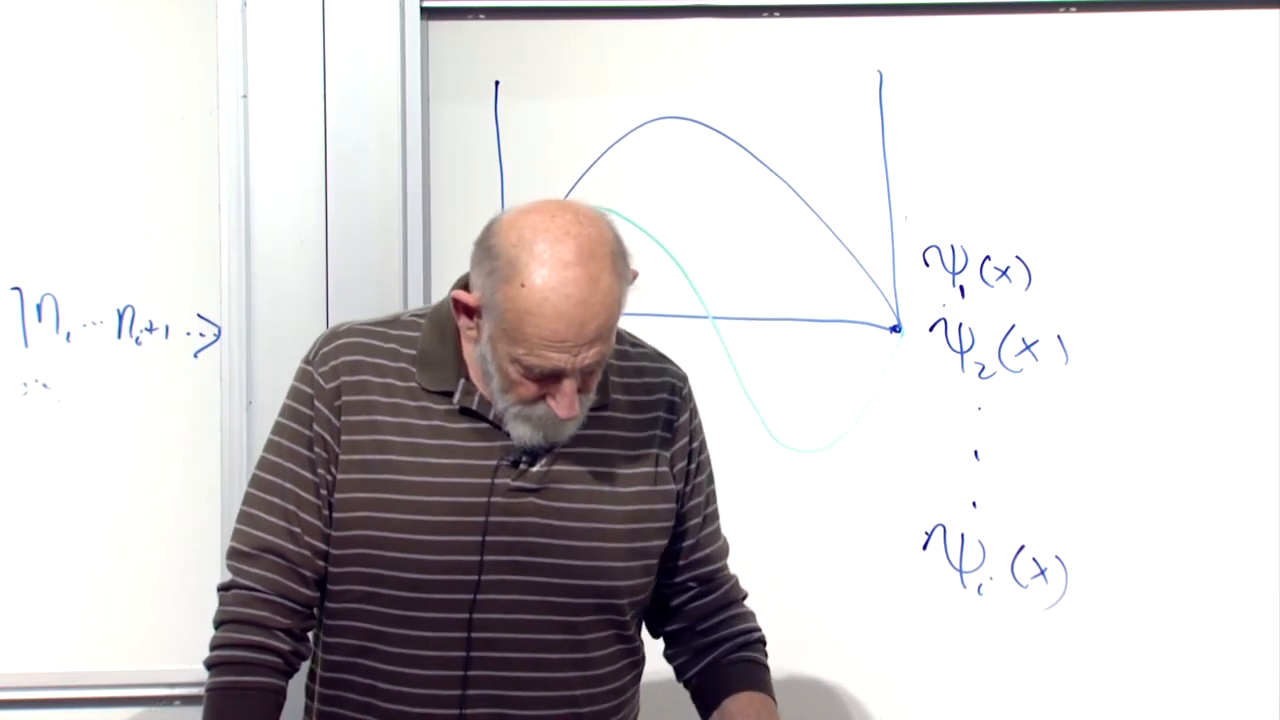
\includegraphics[width=0.9\linewidth]{lecture_06_frame_03.png}
\caption{エネルギー増加順に並べた一粒子箱モード。最初のモードは内部節を持たず、二番目は一つ持ち、省略されたより高次のモードは次第により速く振動する。}
\lectureframe{00:43:10}
\end{figure}

同じ構造は、ライブボードによる遮蔽なしに描き直すことができる。
\begin{figure}[htbp]
\centering
\begin{tikzpicture}[x=1cm,y=1cm]
  \draw[thick] (0,0) -- (0,3.8);
  \draw[thick] (7,0) -- (7,3.8);
  \draw[gray!55] (0,2.75) -- (7,2.75);
  \draw[gray!55] (0,1.35) -- (7,1.35);
  \draw[blue!75!black,thick,domain=0:7,samples=120]
    plot (\x,{2.75+0.62*sin(180*\x/7)});
  \draw[teal!70!black,thick,domain=0:7,samples=120]
    plot (\x,{1.35+0.55*sin(360*\x/7)});
  \node[right] at (7.15,3.15) {$\psi_1(x)$};
  \node[right] at (7.15,1.70) {$\psi_2(x)$};
  \node at (3.5,0.45) {$\vdots\quad \psi_i(x)$};
\end{tikzpicture}
\caption{箱モードの定性的スケッチの明快な再構成。縦方向の変位は読みやすさのために固有関数を分離したものであり、追加の物理的座標ではない。}
\end{figure}

添字\(i\)は一粒子状態を表し、粒子や節の数を表すものではない。箱基底の場合、\(i\)はたまたま内部の節の数より1だけ大きい。各状態はエネルギー\(\varepsilon_i\)をもつ。講義の記法に従えば、このエネルギーを\(\hbar\omega_i\)と書くことができ、\(\hbar=1\)と置けば単に\(\omega_i\)と書ける。

\begin{classroomqa}
\lecturetimestamp{00:39:01}
\audiencequestion{先ほどの独立性の仮定は厳密だったのか、また添字\(i\)は原子中の電子の可能な状態を表しうるのか。}
\lecturerresponse{独立モードの構成では、異なるモード間の交換関係は厳密である。添字は一粒子原子状態を表しうる。しかし粒子が相互作用するならば、単純な独立モードのハミルトニアンはもはや全体像ではない。}
\end{classroomqa}

\begin{classroomqa}
\lecturetimestamp{00:40:34}
\audiencequestion{箱の中の粒子はボソンか。}
\lecturerresponse{ボソンでありうるが、粒子が1個なら統計は問題にならない。排他性と交換は、同一の粒子が複数あるときに初めて意味をもつ。}
\end{classroomqa}

\section{箱モードからフォック空間へ}

ここで、箱の中に任意個の同一ボソンを許す。ある数\(n_1\)が\(\psi_1\)を占め、ある数\(n_2\)が\(\psi_2\)を占め、以下同様である。したがって基底状態は
\begin{equation}
|n_1,n_2,n_3,\ldots\rangle.
\end{equation}
これはすでに多振動子に対して用いた記法そのものである。この同一性は構造的である。すなわち、各一粒子状態に1つの振動子を対応させ、振動子の励起数をその状態を占める粒子数と同一視する。

ここでボソンが本質的であるのは、各\(n_i\)が任意の非負整数でありうるからである。フェルミオンの場合、各一粒子状態は空か単一占有かのいずれかであり、二重占有は決してない。したがって通常の振動子代数をそのまま用いることはできない。

演算子はここで、占有数基底への作用によって定義できる。演算子\(a_i^\dagger\)は一粒子状態\(i\)に1個の粒子を生成し、\(a_i\)は1個を消滅させる。
\begin{align}
a_i^\dagger|n_1,\ldots,n_i,\ldots\rangle
&=\sqrt{n_i+1}\,|n_1,\ldots,n_i+1,\ldots\rangle, \\
a_i|n_1,\ldots,n_i,\ldots\rangle
&=\sqrt{n_i}\,|n_1,\ldots,n_i-1,\ldots\rangle.
\end{align}
これは後付けの類推ではない。この基底上でのボソン生成消滅演算子の定義である。基底が空間を張るため、この定義は線形性によりすべての状態への作用を定める。

\begin{classroomqa}
\lecturetimestamp{00:47:11}
\audiencequestion{\(n_1,n_2,n_3\)は量子状態か。}
\lecturerresponse{ラベル\(1,2,3,\ldots\)は一粒子状態を識別する。記号\(n_1,n_2,n_3,\ldots\)はそれらの状態を占める粒子数である。状態ラベルとその占有数を区別し続けることが、主な記法上の負担である。}
\end{classroomqa}

\subsection{平方根は何をするのか}

因子\(\sqrt{n_i+1}\)は追加の粒子や別個の物理過程を表すものではない。それは演算子に正しい規格化と代数を与える。1モードでは
\begin{align}
a a^\dagger|n\rangle
&=a\bigl(\sqrt{n+1}\,|n+1\rangle\bigr) \\
&=(n+1)|n\rangle,
\end{align}
一方
\begin{equation}
a^\dagger a|n\rangle=n|n\rangle.
\end{equation}
したがってそれらの差は\(|n\rangle\)であり、\([a,a^\dagger]=1\)によって要求される通りである。2つの梯子演算子は、ごく大まかにはそれぞれ\(\sqrt n\)の程度であり、それらの積が\(n\)の程度の数演算子を与えるからである。

\begin{classroomqa}
\lecturetimestamp{00:47:52}
\audiencequestion{平方根因子にはどのような具体的な物理的意味があるのか。}
\lecturerresponse{それは主として数学的な規格化である。それは占有状態が規格化されること、\(a^\dagger a\)が固有値\(n\)をもつこと、そして梯子演算子が振動子の交換関係を満たすことを保証する。ときに数学こそが必要な意味である。}
\end{classroomqa}

\begin{classroomqa}
\lecturetimestamp{00:52:25}
\audiencequestion{生成消滅演算子はその性質と基底への作用によってのみ定義されたのか。}
\lecturerresponse{はい。定義はより原始的な描像から生じる必要はない。その価値は帰結によって試される。完全な基底への作用を定義すれば、演算子は至る所で定義される。そしてこれらの定義は望ましい交換関係を再現する。}
\end{classroomqa}

\begin{classroomqa}
\lecturetimestamp{00:53:22}
\audiencequestion{なぜ\(a_i\)は粒子を別の状態へ移すだけでなく消滅させるのか。}
\lecturerresponse{\(a_i\)は状態\(i\)の占有数を下げるように定義されているからである。有用な問いは、なぜある定義が真であるかではなく、なぜそれが有用であるかである。それが有用なのは、放出と吸収には粒子数を変える演算子が必要だからである。光子は放射が放出されるときに生成され、吸収されるときに消滅する。}
\end{classroomqa}

すべての占有数状態が張る空間は\emph{フォック空間}である。それは真空、すべての一粒子状態、すべての二粒子状態などを、固定された上限なしに含む：
\begin{equation}
\mathcal F=\mathcal H_0\oplus\mathcal H_1\oplus\mathcal H_2\oplus\cdots.
\label{eq:l06-fock-space}
\end{equation}
直和の記法は、通常の\(N\)粒子波動関数が明示しなかったことを明示する。すなわち、すべての粒子数セクターが一つの状態空間に属するのである。

\begin{classroomqa}
\lecturetimestamp{00:54:56}
\audiencequestion{演算子を占有数固有ベクトル上で定義すれば、任意のベクトル上での演算子が決まり、振動子の交換関係もそれに従うのか。}
\lecturerresponse{そのとおりである。占有数ベクトルは基底をなすので、線形性によって定義はフォック空間全体に拡張される。その基底に作用させることでボソンの交換関係が検証される。各一粒子状態は一つの振動子で表され、その振動子の占有数はその状態にある粒子の数である。}
\end{classroomqa}

\subsection{真空と自由ハミルトニアン}

フォック真空は、どの一粒子状態にも粒子が存在しない状態である：
\begin{equation}
|0\rangle=|0,0,0,\ldots\rangle,
\qquad a_i|0\rangle=0.
\end{equation}
ここで\emph{基底状態}という語は誤解を招きうる。最低の\emph{一粒子}状態はモード\(i=1\)である。フォック真空はそのモードにも粒子を持たない。もし粒子が最低モードを占めていれば、\(a_1\)はそれを取り除き、系を真空に戻すことができる。

\begin{classroomqa}
\lecturetimestamp{00:56:19}
\audiencequestion{占有数言語における真空とは何か。最低の一粒子状態は占有されているのか。}
\lecturerresponse{真空ではすべての占有数がゼロに等しく、すべての\(a_i\)によって消滅させられる。最低の一粒子モードは真空では占有されていない。もしそれが占有されていれば、その消滅演算子はその粒子を取り除くことができる。}
\end{classroomqa}

非相互作用粒子では、全エネルギーは加法的である。状態\(i\)にある一粒子がエネルギー\(\hbar\omega_i\)を持つならば、
\begin{align}
H
&=\sum_i \hbar\omega_i N_i \\
&=\sum_i \hbar\omega_i a_i^\dagger a_i.
\label{eq:l06-free-fock-hamiltonian}
\end{align}
二つの等価な読み方がある。それは振動子エネルギーの和であり、一粒子状態ごとに一つの振動子がある。またそれは一粒子エネルギーの和であり、それぞれがそのエネルギーを持つ粒子の数で掛けられている。

場の理論の記法では、\(a_i^\dagger\)は通常生成演算子と呼ばれ、\(a_i\)は消滅演算子と呼ばれる。古い\(a_+\)および\(a_-\)という記法も同じことを言っている。

\section{場が現れる前の明確化}

休憩後のいくつかの質問は、新しい振動子的な帳簿付けを、振動子ポテンシャル中を運動する通常の粒子から区別する。

\begin{classroomqa}
\lecturetimestamp{01:06:09}
\audiencequestion{箱の中の粒子のエネルギー準位は等間隔ではないのに、調和振動子はどこにあるのか。}
\lecturerresponse{一粒子エネルギー\(\omega_i\)は等間隔である必要はない。しかし、各固定モード\(i\)について、そのモードにあるゼロ個、一個、二個、三個の非相互作用粒子のエネルギーは\(0,\omega_i,2\omega_i,3\omega_i\)である。その占有数の梯子が振動子である。それは一つの粒子を調和振動子ポテンシャルに置くこととは異なる。}
\end{classroomqa}

\begin{classroomqa}
\lecturetimestamp{01:08:38}
\audiencequestion{この構成はフーリエ分解と関係があるのか。}
\lecturerresponse{深く関係している。一粒子基底が運動量モードからなるとき、モード関数はサイン、コサイン、または複素指数関数であり、\(a_i\)はフーリエ係数の量子類似物である。一般の基底は三角関数である必要はないが、展開の論理は同じである。}
\end{classroomqa}

\begin{classroomqa}
\lecturetimestamp{01:09:07}
\audiencequestion{すべての粒子に同じエネルギーが割り当てられているのか。また相互作用は含まれているのか。}
\lecturerresponse{同じ一粒子状態を占める粒子は同じエネルギーを持つが、異なる状態にある粒子は一般には同じエネルギーを持たない。今のところ粒子は自由である。すなわち相互作用しない。相互作用があればポテンシャルエネルギーの項が加わるので、ハミルトニアンはもはや式~\eqref{eq:l06-free-fock-hamiltonian}の加法的な和だけではなくなる。}
\end{classroomqa}

\begin{classroomqa}
\lecturetimestamp{01:10:26}
\audiencequestion{各振動子にあった零点エネルギーの半量子はどうなったのか。}
\lecturerresponse{それはハミルトニアンにおける付加的な定数である。定数はすべての演算子と可換であるから、ハイゼンベルクの運動方程式を変えず、通常の非重力測定はエネルギー差に依存する。特別な目的には重要でありうるが、ここで展開している構成には影響しない。}
\end{classroomqa}

自由理論はすでに並外れた力をもつ簿記の道具である。それは多数の粒子だけでなく、状態を変え、現れ、消え、あるいは異なる全粒子数の重ね合わせに存在する粒子をも追跡する。適切なエルミート結合は測定可能であるから、演算子は単なる簿記の記号以上のものであるが、簿記という見方は有用な第一の直観である。

\begin{classroomqa}
\lecturetimestamp{01:14:03}
\audiencequestion{場の理論と量子場の理論は歴史的にどこから来たのか。}
\lecturerresponse{簡潔な歴史的経路は、ファラデーの電場と磁場の物理的描像と、古典場に対するマクスウェル方程式から始まる。プランクは熱放射を研究する中でエネルギー量子を導入し、アインシュタインはその量子化を電磁場そのもの、および光量子と同一視した。その後、ハイゼンベルク、パウリ、とりわけディラックが、1920年代の終わりごろに現代的な演算子の枠組みをまとめるのに寄与した。紫外発散と放射の量子的記述は、決定的な初期の問題の一つであった。これは完全な優先権の割り当てではなく、概略的な歴史である。}
\end{classroomqa}

この歴史的な流れは、なぜ振動子が繰り返し現れるかも説明する。空洞内の古典放射は基準モードに分解される。それらのモードを量子化すると、その励起数が光子数になる。モードを占める数学的な量子は物理的な粒子になる。

\section{ボソン場の演算子}

\(\{\psi_i(x)\}\)を一粒子波動関数の完全正規直交基底とする。
\begin{equation}
\boxed{\Psi(x)=\sum_i a_i\,\psi_i(x)}
\label{eq:l06-field-annihilation}
\end{equation}
を定義し、そのエルミート共役を
\begin{equation}
\boxed{\Psi^\dagger(x)=\sum_i a_i^\dagger\,\psi_i^*(x)}.
\label{eq:l06-field-creation}
\end{equation}
とする。

\begin{figure}[htbp]
\centering
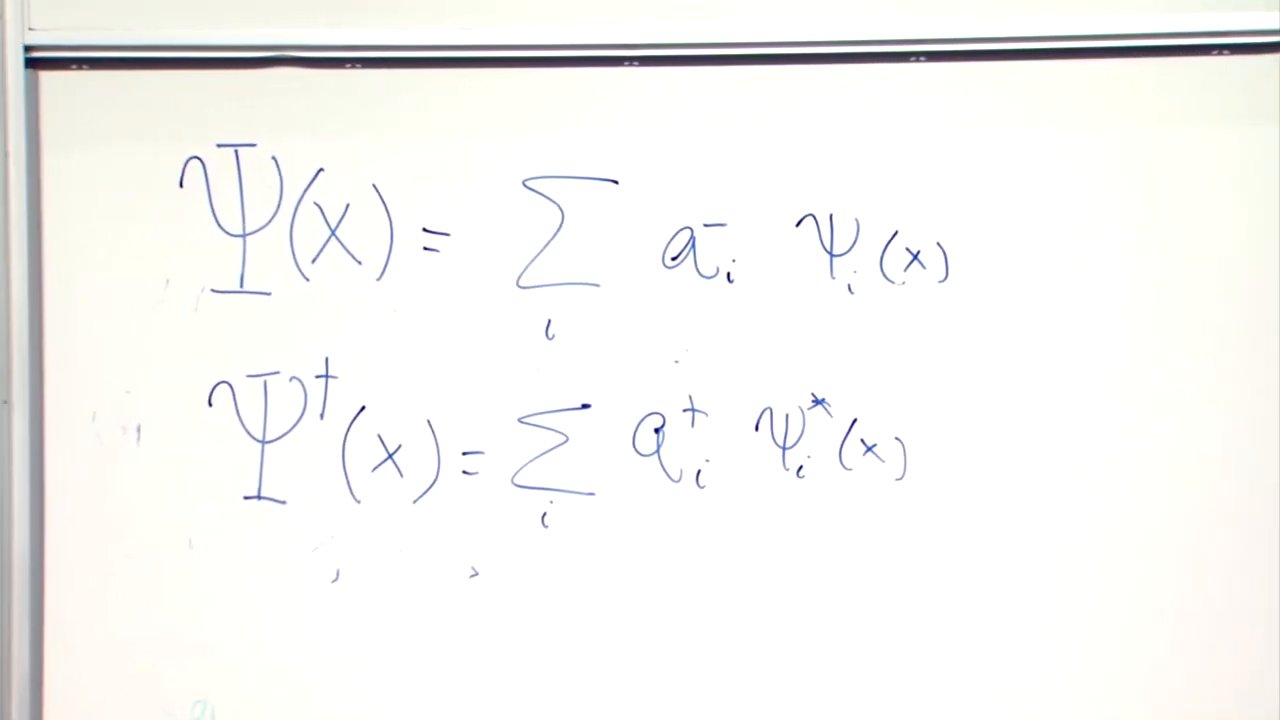
\includegraphics[width=0.9\linewidth]{lecture_06_frame_04.png}
\caption{消滅場とそのエルミート共役の完全なモード展開。式~\eqref{eq:l06-field-annihilation}と\eqref{eq:l06-field-creation}は、組版された形で同じ演算子と複素共役の構造を保っている。}
\lectureframe{01:25:15}
\end{figure}

任意の固定された位置\(x\)に対して、各\(\psi_i(x)\)は通常の複素数である。演算子としての内容はすべて\(a_i\)と\(a_i^\dagger\)にある。\(x\)が変化するにつれて、空間の各点で異なる演算子が得られる。これが、\(\Psi\)が演算子値関数であるという正確な意味である。

基底関数が平面波であれば、式~\eqref{eq:l06-field-annihilation}と\eqref{eq:l06-field-creation}は量子フーリエ展開である。古典的なフーリエ係数が演算子になったのである。箱の中では、基底は代わりに式~\eqref{eq:l06-box-basis}の正弦関数であってもよい。任意の完全正規直交一粒子基底が使える。

\(\Psi\)も\(\Psi^\dagger\)もエルミートではない。観測可能な場は、
\begin{equation}
\Psi(x)+\Psi^\dagger(x),
\qquad
i\bigl(\Psi^\dagger(x)-\Psi(x)\bigr),
\end{equation}
のようなエルミート結合から作ることができ、観測可能な密度は後に\(\Psi^\dagger(x)\Psi(x)\)のような積から作られる。当面の課題は、まず二つの基本的な場が何をするかを理解することである。

\begin{classroomqa}
\lecturetimestamp{01:23:14}
\audiencequestion{右辺のモード関数が通常の波動関数であるのに、なぜ左辺が演算子になりうるのか。}
\lecturerresponse{関数\(\psi_i(x)\)は、\(x\)が選ばれれば数である。因子\(a_i\)は演算子である。数と演算子の積は演算子であり、したがって和も演算子である。\(x\)を変化させると演算子の族全体が得られる。}
\end{classroomqa}

\section{場がすること}

消滅場は真空を直ちに消す。
\begin{equation}
\Psi(x)|0\rangle
=\sum_i\psi_i(x)a_i|0\rangle
=0.
\label{eq:l06-field-kills-vacuum}
\end{equation}
生成場はもっとずっと情報に富むことをする。

\(|i\rangle\)を波動関数
\begin{equation}
\langle x|i\rangle=\psi_i(x).
\end{equation}
をもつ一粒子状態とする。一粒子基底の完全性により
\begin{equation}
\sum_i|i\rangle\langle i|=1.
\label{eq:l06-completeness}
\end{equation}
この恒等式を位置固有状態に適用すると、
\begin{align}
|x\rangle
&=\sum_i|i\rangle\langle i|x\rangle \\
&=\sum_i\psi_i^*(x)|i\rangle.
\label{eq:l06-position-expansion}
\end{align}
フォックの言葉では、一粒子モード状態は
\begin{equation}
|i\rangle=a_i^\dagger|0\rangle.
\end{equation}
である。これを式~\eqref{eq:l06-position-expansion}に代入すると、
\begin{align}
|x\rangle
&=\sum_i\psi_i^*(x)a_i^\dagger|0\rangle \\
&=\Psi^\dagger(x)|0\rangle.
\label{eq:l06-local-creation}
\end{align}
したがって\(\Psi^\dagger(x)\)は\(x\)に局在する粒子を生成し、\(\Psi(x)\)はそこで粒子を一つ取り除く。位置固有状態はデルタ関数的に局在し、一般化された非規格化状態である。物理的に局在した粒子は、規格化可能な波束で場をならすことによって得られる。\editorialnote{講義は理想的な位置固有状態の言葉で話している。波束に関する但し書きは、議論を変えることなく標準的な数学的意味を記録したものである。}

\begin{classroomqa}
\lecturetimestamp{01:36:26}
\audiencequestion{どのような種類の粒子が生成されるかを指定する情報はどこにあるのか。\(x\) における状態はデルタ関数的に局在しているのか。}
\lecturerresponse{各粒子種には別々の場が割り当てられるので、粒子の同一性はどの場が用いられるかによって担われる。引数 \(x\) はそれがどこで生成されるかを指定する。理想的な位置基底では、生成された状態はデルタ関数的局在をもつ。}
\end{classroomqa}

ボソン種の例には光子、重力子、ヒッグス粒子、グルーオンが含まれるが、現実的な場は内部指数も担う。光子でさえ偏極ラベルを必要とする。簡略化されたスカラー場の記法はそれらの余分なラベルを抑制し、生成の原理が見えるようにしている。

\subsection{真空は零ベクトルではない}

方程式
\begin{equation}
\Psi(x)|0\rangle=0
\end{equation}
には、零で表される二つの非常に異なる対象が含まれている。ケット \(|0\rangle\) は真空である。すなわち
\begin{equation}
\langle0|0\rangle=1.
\end{equation}
を満たす規格化された物理的状態である。右辺の結果は零ベクトルである。そのノルムは零であり、規格化できず、物理的状態を表さない。

その違いは加法の下で鮮明になる。零ベクトルを一粒子状態に加えても何も変わらない。真空を一粒子状態に加えると、異なる粒子数セクターの真の重ね合わせが得られる。規格化された係数を用いると、
\begin{equation}
|\chi\rangle=\frac{1}{\sqrt2}\bigl(|0\rangle+|1\rangle\bigr)
\end{equation}
は零粒子と一粒子に対して等しい確率をもつ。これは \(|1\rangle\) と同じではない。

\begin{classroomqa}
\lecturetimestamp{01:37:23}
\audiencequestion{もし \(x\) に粒子が存在しないなら、\(\Psi(x)\) は単に何もしないのか。結果が零になるとはどういう意味か。}
\lecturerresponse{それは元の状態を返すのではない。零ベクトルを返す。真空は空の空間を記述する規格化された状態であり、零ベクトルは長さが零で、いかなる物理的状態も記述しない。零ベクトルに作用する任意の演算子は零ベクトルを返す。}
\end{classroomqa}

\begin{classroomqa}
\lecturetimestamp{01:39:00}
\audiencequestion{零ベクトルではなく真空を一粒子状態に加えるとどうなるか。}
\lecturerresponse{異なる粒子数の振幅をもつ重ね合わせが得られる。対照的に、零ベクトルを加えても一粒子状態は変わらない。\(|0\rangle\) における記号は占有数零を名指すのであり、零ベクトルを意味するのではない。}
\end{classroomqa}

\begin{classroomqa}
\lecturetimestamp{01:41:56}
\audiencequestion{場の展開において、モード関数とその生成演算子または消滅演算子の順序は重要ですか。モード関数は複素数ですか。}
\lecturerresponse{モード関数は通常の数であり、したがってすべての演算子と可換であるから、順序は重要ではない。一般にモード関数は複素数であり得る。選んだ基底が実数か複素数かは、一粒子Schr\"odinger問題に依存する。}
\end{classroomqa}

\subsection{二粒子とボソン対称性の出現}

\(x\) に一粒子を、\(y\) にもう一粒子を生成するには、二度作用させる。
\begin{equation}
|x,y\rangle
=\Psi^\dagger(y)\Psi^\dagger(x)|0\rangle.
\label{eq:l06-two-particle-state}
\end{equation}
点は一致しても異なってもよい。基礎となる生成演算子は可換であるから、
\begin{align}
[\Psi^\dagger(x),\Psi^\dagger(y)]
&=\sum_{i,j}\psi_i^*(x)\psi_j^*(y)
[a_i^\dagger,a_j^\dagger] \\
&=0.
\end{align}
したがって
\begin{equation}
\Psi^\dagger(y)\Psi^\dagger(x)|0\rangle
=\Psi^\dagger(x)\Psi^\dagger(y)|0\rangle.
\label{eq:l06-boson-exchange}
\end{equation}
二粒子の順序を交換しても何も変わらない。これはまさにボソン交換対称性である。したがって我々は振動子代数から出発して、可換な生成演算子から構成される粒子がボソンであることを\emph{導出}できたことになる。フェルミオンには代わりに反可換な演算子が必要となる。

\begin{classroomqa}
\lecturetimestamp{01:42:37}
\audiencequestion{一粒子状態に二つ目の粒子を加えるにはどうすればよいか。}
\lecturerresponse{もう一つの生成場を作用させる。\(y\)に粒子を加えるには、\(\Psi^\dagger(y)\)を\(\Psi^\dagger(x)\)の左側に置いて作用させる。その結果は式~\eqref{eq:l06-two-particle-state}の二粒子状態である。}
\end{classroomqa}

\begin{classroomqa}
\lecturetimestamp{01:46:04}
\audiencequestion{二つの生成場の可換性は、二粒子状態を対称化することと完全に等価か。}
\lecturerresponse{はい。それは \(x\) に一粒子、\(y\) に一粒子をもつ状態を、ラベルを交換して得られる状態と同一にする。これが同一ボソンの定義的な交換性質である。}
\end{classroomqa}

\begin{classroomqa}
\lecturetimestamp{01:46:32}
\audiencequestion{これは \(x\) と \(y\) の粒子が同じ種類のボソンでなければならないことを意味するか。}
\lecturerresponse{はい。引数 \(x\) と \(y\) は位置であり、一方の場は一つの種を記述する。異なる種、および二つの光子偏極のような追加のラベルには、別個の場の成分が必要である。}
\end{classroomqa}

\section{なぜ粒子数が変わりうることが重要か}

もしある問題で粒子の数がいつまでもちょうど37個のままなら、場の言葉は必須ではなく、補助的な記法にすぎない。その真価が現れるのは、粒子が放出・吸収されうるとき、とりわけ粒子数自体が量子変数であるときである。フォック空間では、次の形の状態を扱うことができる。
\begin{equation}
|\Phi\rangle
=c_0|0\rangle+c_1|1\rangle+c_2|2\rangle+\cdots,
\qquad
\sum_{n=0}^{\infty}|c_n|^2=1.
\end{equation}
レーザー場はその重要な例である。一般にそれは、光子数が一つの値に確定した状態ではなく、異なる粒子数の部分空間に属する状態の重ね合わせである。

粒子と場の橋渡しは今や明示的である。モード演算子はエネルギー固有状態における粒子を数え、変化させる。場はそれらの演算子を完全系の波動関数と組み合わせ、指定された位置で粒子を生成または消滅させることができるようにする。調和振動子の代数は、ボソン量子場の初等的言語となった。

\chapter{粒子から単純な量子場へ}

もう一度、単純な量子場を構築しよう。ただし、少し異なる角度からである。量子場理論への道は二つある。粒子から出発して、なぜ場が粒子にとって自然な言語なのかを発見する道と、波動場から出発して、なぜその励起が量子として現れるのかを発見する道である。どちらの道も有用である。ここでは最初の道にとどまる。

通常の量子力学は、一粒子、二粒子、あるいはその他の任意の固定された数を記述できる。自然はその制限を尊重しない。部屋の中の光子の数は、照明が放射を放出または吸収するたびに変化する。不安定な粒子は崩壊する。例えばベータ崩壊では、
\begin{equation}
n\longrightarrow p+e^-+\bar{\nu}_e,
\end{equation}
であるから、複数の粒子種の個数が同時に変化する。したがって我々は、あらゆる可能な占有数を含み、最終的にはそれらの間を移る過程をも含むのに十分大きな一つの量子力学を望む。

当面は大幅に単純化する。非相対論的な一つの粒子種がある。まずその状態空間を、任意の粒子数を保持できるように拡大し、その後になってから、より多くの粒子種、相対論、散乱、崩壊について論じる。数学はどれも特に難しいわけではないが、視点の変化は抽象的である。記法が考えを隠してしまわないように、十分ゆっくりと歩を進める価値がある。

\section{一粒子の出発点}

状態 \(|\psi\rangle\) にある一つの粒子から始める。その位置空間の波動関数は
\begin{equation}
\psi(x)=\langle x|\psi\rangle.
\label{eq:l07-wavefunction}
\end{equation}
である。この小文字の \(\psi\) は通常の複素数値関数である。それはまだ量子場ではなく、多粒子状態空間上の演算子でもない。

ボルンの規則によれば、
\begin{equation}
\rho_\psi(x)=|\psi(x)|^2=\psi^*(x)\psi(x)
\label{eq:l07-born-density}
\end{equation}
は粒子を \(x\) に見出す確率密度である。規格化された状態に対して、
\begin{equation}
\int dx\,\psi^*(x)\psi(x)=1.
\label{eq:l07-one-particle-normalization}
\end{equation}
である。右辺は全確率である。この問題にはちょうど一つの粒子しか含まれないので、それは粒子の数にもたまたま等しい。この一致は、ここでは自明であるが、後に有用な手がかりとなるであろう。

\begin{classroomqa}
\lecturetimestamp{00:09:13}
\audiencequestion{なぜ確率密度は \(\psi^*(x)\psi(x)\) の形をとらなければならないのか。}
\lecturerresponse{それは量子力学の公理の一つであるボルンの規則である。位置の結果 \(x\) に対する振幅は \(\langle x|\psi\rangle\) であり、確率密度はその絶対値の二乗である。それは後に用いる場の構成から導かれるものではない。}
\end{classroomqa}

\section{モード、直交性、完全性}

一粒子ヒルベルト空間には多くの有用な基底がある。位置固有状態は一つの基底をなす。任意のエルミート演算子の固有状態は、縮退と連続スペクトルに対する通常の但し書きとともに、別の基底をなす。エネルギーがまもなく重要になるので、一粒子エネルギー固有状態の完全正規直交系を選ぶ。
\begin{equation}
|1\rangle,\ |2\rangle,\ldots,
\qquad
\psi_i(x)=\langle x|i\rangle.
\end{equation}

箱の中の粒子は、添字 \(i\) を具体的なものにする。基底状態の波動関数は内部に節を持たず、次の状態は一つ持ち、より高い状態はより速く振動する。理想的な無限井戸に対して、それらは本質的に正弦波である。

\begin{figure}[htbp]
\centering
\includegraphics[width=0.94\linewidth]{lecture_07_frame_01.png}
\caption{講義板の上の箱のモード。左側の残りは一粒子ボルン密度と規格化であり、右側の井戸は \(\psi_1(x)\)、\(\psi_2(x)\)、および一般ラベル \(\psi_i(x)\) を示す。}
\lectureframe{00:08:25}
\end{figure}

同じモード構造を、ライブ板の遮蔽から分離することができる。
\begin{figure}[htbp]
\centering
\begin{tikzpicture}[x=1cm,y=1cm]
  \draw[thick] (0,0) -- (0,4.0);
  \draw[thick] (7,0) -- (7,4.0);
  \draw[gray!55] (0,2.85) -- (7,2.85);
  \draw[gray!55] (0,1.35) -- (7,1.35);
  \draw[blue!75!black,thick,domain=0:7,samples=120]
    plot (\x,{2.85+0.62*sin(180*\x/7)});
  \draw[teal!70!black,thick,domain=0:7,samples=120]
    plot (\x,{1.35+0.55*sin(360*\x/7)});
  \node[right] at (7.15,3.20) {$\psi_1(x)$};
  \node[right] at (7.15,1.70) {$\psi_2(x)$};
  \node at (3.5,0.38) {$\vdots\quad\psi_i(x)$};
\end{tikzpicture}
\caption{定性的な箱のスケッチの清書。縦方向のずれは、表示のために二つの波動関数を分けているだけである。}
\end{figure}

正規直交性は
\begin{equation}
\int dx\,\psi_i^*(x)\psi_j(x)=\delta_{ij}.
\label{eq:l07-orthonormality}
\end{equation}
である。\(i=j\) ならば、状態は規格化されており、積分は 1 である。\(i\ne j\) ならば、二つの状態は直交しており、積分は消える。

完全性は、同じく重要な命題
\begin{equation}
\sum_i |i\rangle\langle i|=\mathbf 1.
\label{eq:l07-resolution}
\end{equation}
である。各 \(|i\rangle\langle i|\) は一つの基底方向への射影であり、完全基底にわたる和は恒等演算子である。任意のベクトルに作用させることは、そのベクトルを成分に分解し、再び組み立てるだけである。

ここで式~\eqref{eq:l07-resolution}を二つの位置状態ではさむ。
\begin{align}
\langle y|x\rangle
&=\sum_i\langle y|i\rangle\langle i|x\rangle \\
&=\sum_i\psi_i(y)\psi_i^*(x) \\
&=\delta(y-x).
\label{eq:l07-position-completeness}
\end{align}
星印は、ブラケットの順序が \(\langle i|x\rangle\) である因子に付く。\(x\) と \(y\) を入れ替えると、複素共役ではあるが等価な形が得られる。したがって、任意の完全正規直交基底はデルタ関数の表現を与える。正弦、余弦、振動子波動関数、エネルギー固有関数はすべて同じ役割を果たす。

\begin{classroomqa}
\lecturetimestamp{00:13:43}
\audiencequestion{完全性の和における二番目の波動関数は複素共役を伴うべきか。}
\lecturerresponse{はい。順序 \(\langle y|i\rangle\langle i|x\rangle\) では、因子は \(\psi_i(y)\psi_i^*(x)\) である。ブラケットの順序を見えるように保つことで、星印を推測したり置き忘れたりすることを防げる。}
\end{classroomqa}

これが我々に必要な一粒子の数学である。ここで状態空間を変更する。

\section{より大きな状態空間としてのフォック空間}

多数の同種粒子に対しては、各一粒子モードに何個の粒子が入っているかを記録する基底が便利である：
\begin{equation}
|n_1,n_2,n_3,\ldots\rangle.
\label{eq:l07-fock-basis}
\end{equation}
整数\(n_i\)はモード\(i\)の占有数である。このケットは、凝った記法で書かれた一粒子状態ではない。それはゼロ粒子セクター、すべての一粒子状態、すべての二粒子状態、等々を含む、より大きなヒルベルト空間に属する。そのより大きな空間はフォック空間と呼ばれる。

占有数を変えるために、各モードに対して生成演算子と消滅演算子を導入する：
\begin{equation}
a_i^\dagger,\qquad a_i.
\end{equation}
第一のものはモード\(i\)に粒子を一つ加え、第二のものは粒子を一つ取り除く。この段階では、調和振動子の言葉は帳簿付けの道具である：文字通りの振動するばねが存在する必要はない。振動子代数は、占有数を上げ下げするのに必要な仕組みをまさに与えてくれる。

モード数演算子は
\begin{equation}
\begin{aligned}
N_i&=a_i^\dagger a_i,\\
N_i|n_1,\ldots,n_i,\ldots\rangle
&=n_i|n_1,\ldots,n_i,\ldots\rangle.
\end{aligned}
\end{equation}
真空は
\begin{equation}
|0\rangle\equiv|0,0,0,\ldots\rangle,
\qquad
a_i|0\rangle=0
\quad\text{for every }i.
\label{eq:l07-vacuum}
\end{equation}
したがってモード\(i\)の一粒子状態は
\begin{equation}
|i\rangle=a_i^\dagger|0\rangle.
\label{eq:l07-mode-created}
\end{equation}
同じ記号\(|i\rangle\)は今や、一粒子基底ベクトルとしても、フォック空間の一粒子セクターに埋め込まれたそのベクトルとしても読むことができる。埋め込みは式~\eqref{eq:l07-mode-created}である；周囲の文脈が、どちらの空間が議論されているかを教えてくれる。

\section{モードを場にまとめる}

消滅場と生成場を次で定義する：
\begin{equation}
\Psi(x)=\sum_i \psi_i(x)a_i,
\qquad
\Psi^\dagger(x)=\sum_i \psi_i^*(x)a_i^\dagger.
\label{eq:l07-field-expansion}
\end{equation}
大文字であることが重要である。小文字の関数\(\psi_i(x)\)は複素数である；大文字の\(\Psi(x)\)はフォック空間上の演算子である。各空間点\(x\)において、式~\eqref{eq:l07-field-expansion}はモード演算子の異なる線形結合を与える。これが位置の演算子値関数の意味である。

自由粒子に対しては、モード関数は平面波\(e^{ikx}\)であってよい。そのとき式~\eqref{eq:l07-field-expansion}はフーリエ展開であるが、そのフーリエ係数が数ではなく演算子である点が異なる。古い用語では、通常の複素数を\(c\)数、量子演算子を\(q\)数と呼ぶ。モード関数は\(c\)数であり、すべてと可換である；\(a_i\)と\(a_i^\dagger\)が演算子としての性格を担う。

\(\Psi\)も\(\Psi^\dagger\)もエルミートではない。それらの随伴は互いに他方である。二つの組み合わせ
\begin{equation}
\Psi+\Psi^\dagger,
\qquad
i(\Psi^\dagger-\Psi)
\label{eq:l07-hermitian-combinations}
\end{equation}
はエルミートであり、観測量を表すことができる。しかし今のところ、場は粒子を局所的に生成し、消滅させ、数える道具として最も有用である。

\begin{classroomqa}
\lecturetimestamp{00:21:05}
\audiencequestion{演算子が\(x\)に依存するとはどういう意味か。}
\lecturerresponse{それは、\(x\)の各値が異なる演算子を選び出すという意味である。空間依存性は通常のモード関数にあり、その結果得られる各線形結合は同じフォック空間に作用する。}
\end{classroomqa}

\section{生成場がすること}

定義は、それが何をするかを問うて初めて有用になる。一粒子セクターの位置固有状態から始め、完全性の分解を挿入する：
\begin{align}
|x\rangle
&=\sum_i |i\rangle\langle i|x\rangle \\
&=\sum_i a_i^\dagger|0\rangle\,\psi_i^*(x) \\
&=\Psi^\dagger(x)|0\rangle.
\label{eq:l07-local-creation}
\end{align}
したがって\(a_i^\dagger\)は確定したモード\(i\)に粒子を生成するのに対し、\(\Psi^\dagger(x)\)は\(x\)に局在した粒子を生成する。理想化された位置基底では、その局在は超関数的である；物理的な準備では狭い波束を用いるであろうが、代数的な意味は同じである。

\begin{classroomqa}
\lecturetimestamp{00:24:48}
\audiencequestion{\(\sum_i|i\rangle\langle i|\)は射影か。}
\lecturerresponse{各項は一つの基底状態への射影である。完全な和はそれ自身が恒等演算子であり、恒等演算子の分解と呼ばれる。それを挿入しても状態は変わらないが、選ばれた基底における状態の成分が露わになる。}
\end{classroomqa}

式~\eqref{eq:l07-local-creation}は場の最初の直接的な粒子解釈である。我々は抽象的な演算子に空間的ラベルを付けただけではない。その空間点に粒子を作る操作を構成したのである。

\begin{classroomqa}
\lecturetimestamp{00:28:20}
\audiencequestion{位置空間の生成場には星印を付けるべきか、それともダガーを付けるべきか。}
\lecturerresponse{演算子の随伴にはダガーを用いる。星印は通常の波動関数\(\psi_i(x)\)の複素共役を表す；ダガーは\(a_i^\dagger\)と\(\Psi^\dagger(x)\)に付けるべきである。}
\end{classroomqa}

\begin{classroomqa}
\lecturetimestamp{00:28:36}
\audiencequestion{モード展開において生成演算子を波動関数の前後に動かしてよいか。}
\lecturerresponse{よい。\(\psi_i(x)\)は\(c\)数であるから、すべての演算子と可換である。\(a_i\)と\(a_j^\dagger\)のような非可換演算子の順序を変えるときだけ注意が必要である。}
\end{classroomqa}

\section{確率密度から粒子密度へ}

ではここで場をいじってみよう。最初の自然な表式は
\begin{equation}
\int dx\,\Psi^\dagger(x)\Psi(x).
\end{equation}
である。これは一粒子の規格化積分のように見えるが、その因子は今や演算子である。順序を変えずにモード展開を代入すると、
\begin{align}
\int dx\,\Psi^\dagger(x)\Psi(x)
&=\int dx
\left(\sum_i a_i^\dagger\psi_i^*(x)\right)\\
&\qquad\times\left(\sum_j a_j\psi_j(x)\right) \\
&=\sum_{i,j}a_i^\dagger a_j
\int dx\,\psi_i^*(x)\psi_j(x) \\
&=\sum_{i,j}a_i^\dagger a_j\,\delta_{ij} \\
&=\sum_i a_i^\dagger a_i.
\label{eq:l07-number-derivation}
\end{align}
となる。したがって総数演算子は
\begin{equation}
N=\sum_i N_i
=\int dx\,\Psi^\dagger(x)\Psi(x).
\label{eq:l07-total-number}
\end{equation}
である。ここで議論している状態では、有限エネルギーの励起は、モードエネルギーが十分高くなると占有数が消えていくので、可能なモードのリストが無限であっても、この総数は通常有限である。

被積分関数は局所的な粒子密度演算子である：
\begin{equation}
n(x)=\Psi^\dagger(x)\Psi(x).
\label{eq:l07-density}
\end{equation}
厳密に言えば、数学的な点で密度を測定することはない。小さな領域\(R\)に対しては、
\begin{equation}
N_R=\int_R dx\,n(x),
\label{eq:l07-regional-number}
\end{equation}
すなわちその領域内の粒子数を測定する。他の量子可観測量と同様に、\(N_R\)は任意の状態で確定した値をもつ必要はない。繰り返しの準備は異なる結果をもたらしうる。

\begin{classroomqa}
\lecturetimestamp{00:36:27}
\audiencequestion{\(\Psi^\dagger(x)\Psi(x)\)は多粒子確率密度なのか。}
\lecturerresponse{その直接的な意味は粒子密度である。多粒子確率振幅は一般にすべての粒子座標に依存する。これに対して局所的な双線形は、その領域にわたって積分されるとき、小さな領域内の粒子を数える。}
\end{classroomqa}

\begin{classroomqa}
\lecturetimestamp{00:38:28}
\audiencequestion{演算子\(a_i\)と\(a_i^\dagger\)は状態ベクトルにのみ作用し、一粒子波動関数には作用しないのか。}
\lecturerresponse{そのとおりである。それらは\(|n_1,n_2,\ldots\rangle\)のようなフォック空間の状態に作用する。それらに掛かる一粒子モード関数は通常の数であり、これらの昇降演算子が作用する対象ではない。}
\end{classroomqa}

占有数ケットは基底をなすが、最も一般的な状態ではない。それらは重ね合わせられうる。同じ総数がモード間で異なる分配をされる重ね合わせも含まれる。光子のような中性の種については、異なる総粒子数の重ね合わせも可能である。式~\eqref{eq:l07-regional-number}の演算子は、そのようなあらゆる状態において同じ操作的意味を保つ。

\begin{classroomqa}
\lecturetimestamp{00:40:01}
\audiencequestion{粒子密度を総数で割ると、\(x\)に粒子を見出す確率密度になるのか。}
\lecturerresponse{固定された\(N\)で大占有数の設定では、\(N_R/N\)は相対頻度であり、通常は一粒子確率を非常によく追跡する。それは一つの測定結果を確率と同一視する演算子の恒等式ではない。測定される計数は変動し、独立粒子描像では典型的には\(\sqrt N\)程度の量であり、例外的な試行は、そのような試行が起こりにくいとしても、確率から大きく異なりうる。}
\end{classroomqa}

\begin{classroomqa}
\lecturetimestamp{00:42:25}
\audiencequestion{一電子状態と零電子状態の重ね合わせで電荷保存はどうなるのか。}
\lecturerresponse{それは固定された電荷の閉じたセクターに用いられる種類の重ね合わせではない。同じ総電荷をもつ異なる分配を重ね合わせることはできる。光子は電荷を運ばないので、異なる光子数セクターはそのような問題を引き起こさない。電子数と陽電子数も、正味の電荷が固定されたまま一緒に変化しうる。}
\end{classroomqa}

\section{独立粒子のエネルギー}

次の可観測量はエネルギーである。まず互いに相互作用しない粒子に限定する。これは希薄系ではしばしば良い近似である。光子も原理的には高次過程を通じて相互作用するが、通常の実験室の放射は独立粒子描像が優れて成り立つほど希薄である。

\(\omega_i\)をモード\(i\)における一粒子のエネルギーとし、\(\hbar=1\)とする。モードとは一つの一粒子状態を意味する。このとき全ハミルトニアンは
\begin{equation}
H=\sum_i\omega_i N_i
=\sum_i\omega_i a_i^\dagger a_i.
\label{eq:l07-mode-hamiltonian}
\end{equation}
である。各占有モードは、粒子一つにつきその一粒子エネルギーを一度寄与する。

\begin{classroomqa}
\lecturetimestamp{00:48:16}
\audiencequestion{\(\omega_i\)は位置の関数か。}
\lecturerresponse{いいえ。それはモード\(i\)に付随するエネルギー固有値である。関数\(\psi_i(x)\)は位置に依存し、\(\omega_i\)はどのエネルギー準位が選ばれたかに依存する。}
\end{classroomqa}

値\(\omega_i\)は一粒子の時間に依存しないシュレーディンガー方程式によって決まる。
\begin{equation}
h=-\frac{\nabla^2}{2m}+V(x).
\label{eq:l07-one-particle-h}
\end{equation}
と定義すると、
\begin{equation}
h\psi_i(x)=\omega_i\psi_i(x).
\label{eq:l07-schrodinger-eigenvalue}
\end{equation}
となる。一次元では運動量演算子は\(p=-i\partial_x\)であり、\(p^2/(2m)\)は\(-\partial_x^2/(2m)\)となる。三次元では三つの二階導関数が合わさって\(-\nabla^2/(2m)\)となる。

\begin{figure}[htbp]
\centering
\includegraphics[width=0.94\linewidth]{lecture_07_frame_02.png}
\caption{黒板での\(p^2/(2m)+V(x)\)から一粒子シュレーディンガー固有値方程式の微分形への移行。式~\eqref{eq:l07-schrodinger-eigenvalue}はその整理された再構成である。}
\lectureframe{00:54:10}
\end{figure}

任意の規格化された一粒子波動関数に対して、よく知られた期待値は
\begin{equation}
\langle h\rangle_\psi
=\int dx\,\psi^*(x)h\psi(x).
\label{eq:l07-one-particle-energy-expectation}
\end{equation}
である。多粒子の式は、小文字の波動関数を演算子値の場で置き換えることによって示唆される。これはまだ証明ではない。正しさを今から検証する推測である：
\begin{equation}
H=\int dx\,\Psi^\dagger(x)h\Psi(x).
\label{eq:l07-field-hamiltonian}
\end{equation}

\section{まず答えを書き、次にそれを証明する}

方程式~\eqref{eq:l07-field-expansion}を提案されたハミルトニアンに代入する：
\begin{align}
\int dx\,\Psi^\dagger h\Psi
&=\int dx
\left(\sum_i a_i^\dagger\psi_i^*(x)\right)
h\left(\sum_j a_j\psi_j(x)\right) \\
&=\sum_{i,j}a_i^\dagger a_j
\int dx\,\psi_i^*(x)h\psi_j(x).
\label{eq:l07-h-expanded}
\end{align}
微分演算子\(h\)は\(x\)に依存する波動関数\(\psi_j(x)\)に作用し、モード演算子\(a_j\)には作用しない。シュレーディンガー方程式により、
\begin{equation}
h\psi_j(x)=\omega_j\psi_j(x).
\end{equation}
したがって、
\begin{align}
\int dx\,\Psi^\dagger h\Psi
&=\sum_{i,j}a_i^\dagger a_j\omega_j
\int dx\,\psi_i^*(x)\psi_j(x) \\
&=\sum_{i,j}a_i^\dagger a_j\omega_j\delta_{ij} \\
&=\sum_j\omega_j a_j^\dagger a_j.
\label{eq:l07-h-proof}
\end{align}
これはまさに方程式~\eqref{eq:l07-mode-hamiltonian}である。局所場の表式と全粒子エネルギーの和は同じ演算子である。

\begin{figure}[htbp]
\centering
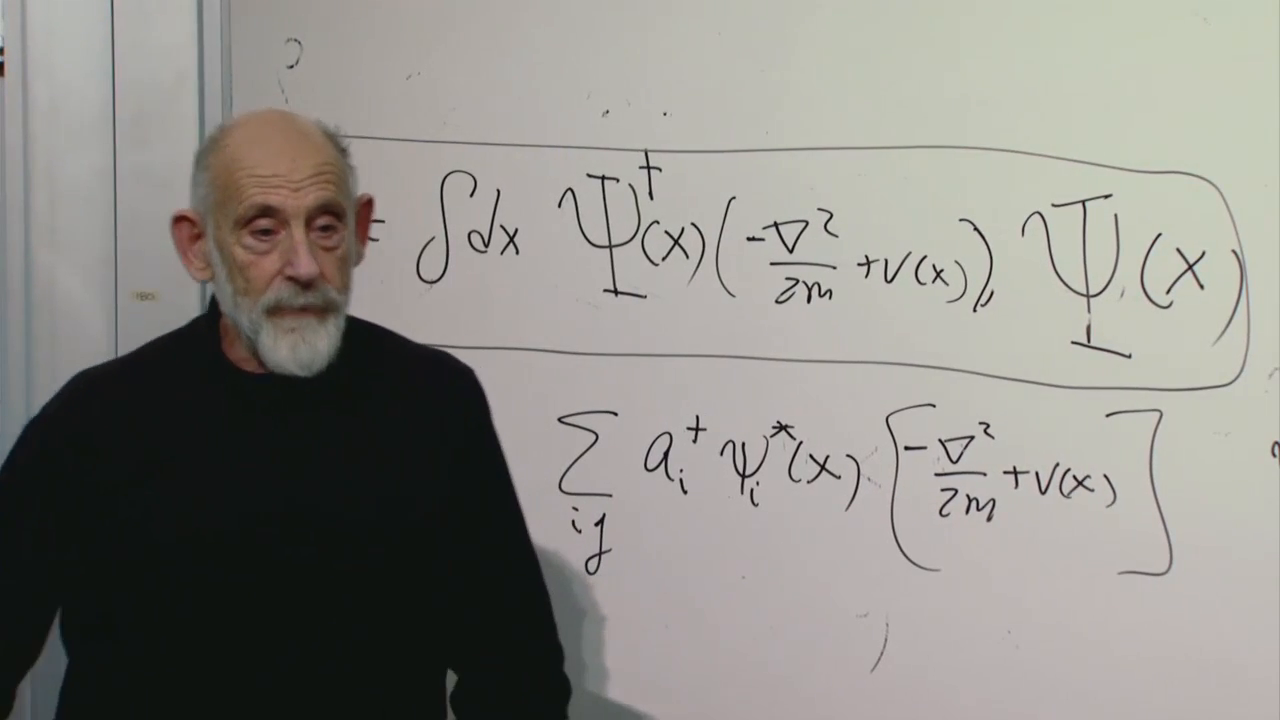
\includegraphics[width=0.94\linewidth]{lecture_07_frame_03.png}
\caption{黒板で強調された場のハミルトニアンと、その下に始まるモード展開による証明。ライブフレームは証拠として保持されている。方程式~\eqref{eq:l07-field-hamiltonian}--\eqref{eq:l07-h-proof}が完全な代数を復元する。}
\lectureframe{01:05:34}
\end{figure}

この導出では、生成演算子が消滅演算子と交換された箇所は一度もない。\(a_i^\dagger a_j\)の順序は最初から最後まで維持されている。自由に動かされた唯一の対象は\(c\)数波動関数とその固有値である。

\section{なぜこれが場なのか}

なぜ\(\Psi(x)\)を場と呼ぶのか。それは空間の各点で定義された演算子値の量であり、それから構成されるエルミート結合や双線形量は局所的可観測量だからである。密度\(n(x)\)と以下の局所エネルギー表式は二つの例である。この言葉の背後に隠れた追加の数学的判定基準はない。

この場は電磁場ではない。それは一粒子モードとハミルトニアン\(p^2/(2m)+V\)を与えた任意の非相対論的種、たとえばゆっくり運動する原子、中性子、陽子、電子を記述する。それらの粒子は対応する場の量子であり、光子が電磁場の量子であるのと同じ構造的な意味においてそうである。

\begin{classroomqa}
\lecturetimestamp{01:02:45}
\audiencequestion{多粒子系から上の式へ移る際、どこで場が入ってきたのか。}
\lecturerresponse{それは方程式~\eqref{eq:l07-field-expansion}で入ってきた：\(\Psi(x)\)は各空間点における演算子である。その後の導出は、その局所積が粒子密度とエネルギー密度を測ることを示している。位置依存性と演算子としての内容が、まさに構成されつつある場の構造である。}
\end{classroomqa}

\section{局所エネルギー密度}

方程式~\eqref{eq:l07-field-hamiltonian}は全エネルギーを空間上の積分として書く：
\begin{equation}
\begin{aligned}
H&=\int dx\,\mathcal H(x),\\
\mathcal H(x)
&=-\frac{1}{2m}\Psi^\dagger(x)\nabla^2\Psi(x)\\
&\quad+V(x)\Psi^\dagger(x)\Psi(x).
\end{aligned}
\label{eq:l07-hamiltonian-density}
\end{equation}
被積分関数はこのハミルトニアンに対する自然な局所エネルギー密度である。その局所形は一意ではない。たとえば部分積分により、運動項は
\begin{equation}
\mathcal H_{\rm kin}(x)
=\frac{1}{2m}\nabla\Psi^\dagger(x)\mathbin{\cdot}\nabla\Psi(x)
\label{eq:l07-kinetic-density}
\end{equation}
に境界項を除いて置き換えられる。通常の境界条件の下で、両方の表式は同じ全ハミルトニアンを与える。これが講義で言及された小さな曖昧さである。

\begin{classroomqa}
\lecturetimestamp{01:05:57}
\audiencequestion{エネルギー密度は全空間にわたって積分しなければならないのか。}
\lecturerresponse{全空間にわたる積分は全エネルギーを与える。より小さな領域にわたる積分は、その領域に割り当てられたエネルギーを与える。ただし、その全積分が同じハミルトニアンとなる局所密度を選ぶ際の通常の曖昧さが伴う。}
\end{classroomqa}

\begin{classroomqa}
\lecturetimestamp{01:06:25}
\audiencequestion{エネルギー式における大文字の\(N_i\)は小文字の\(n_i\)とどう異なるのか。}
\lecturerresponse{\(N_i=a_i^\dagger a_i\)は演算子である。整数\(n_i\)は占有数状態上でのその固有値の一つである。演算子は状態に作用し、その固有値は通常の数である。}
\end{classroomqa}

\begin{classroomqa}
\lecturetimestamp{01:06:46}
\audiencequestion{場のハミルトニアン自体をディラック記法でブラやケットとして書けるか。}
\lecturerresponse{いいえ。ブラとケットは状態ベクトルとその双対を表す。場とハミルトニアンはそれらの状態に作用する演算子である。\(\langle\Phi|H|\Phi\rangle\)のような期待値は両方の種類の対象を用いるのであり、それらを同一視してはならない。}
\end{classroomqa}

\section{一粒子の回復と古典場への接近}

拡大された形式は通常の一粒子量子力学を含んでいる。フォック空間を
\begin{equation}
N|\Phi\rangle=|\Phi\rangle.
\end{equation}
を満たす状態に制限する。その部分空間内では、場の構成はすべての一粒子状態とすべての一粒子予測を再現する。我々は古い理論を置き換えたのではなく、ゼロ個、二個、あるいは任意個の粒子も記述できる空間にそれを埋め込んだのである。

もう一方の極端では、非常に多数のボソンが占有するモードは、近似的に古典的な波のように振る舞うことができる。適切なコヒーレント状態または半古典状態では、期待値
\begin{equation}
\Phi_{\rm cl}(x,t)=\langle\Psi(x,t)\rangle
\end{equation}
は、自由非相対論的理論に対して、古典的に見える方程式
\begin{equation}
i\partial_t\Phi_{\rm cl}(x,t)
=\left(-\frac{\nabla^2}{2m}+V(x)\right)\Phi_{\rm cl}(x,t)
\label{eq:l07-classical-schrodinger}
\end{equation}
に従う。講義はこの関連を導出するのではなく述べるにとどめる。これは量子の集まりと波の場との間の橋渡しである。大きな占有数は相対的な揺らぎを抑え、適切な期待値を古典的に振る舞わせる。

したがって、この形式は簿記であると同時に物理でもある。それはすべての粒子数セクターを整理するが、干渉、エンタングルメント、そして量子粒子から古典的な波が現れることも捉えている。

\begin{classroomqa}
\lecturetimestamp{01:10:43}
\audiencequestion{なぜ生成演算子と消滅演算子は、積分の内部でまるで普通の数のように扱うことができるのか。}
\lecturerresponse{それらは互いに交換されたことは一度もない。通常のモード関数はそれらと可換であり、微分はそれらの関数にのみ作用する。消滅演算子を生成演算子の向こうへ動かすには交換子が必要となり、項が加わる可能性がある。証明の中ではそのような移動は一切行われていない。}
\end{classroomqa}

\section{ディラック記法の間奏}

混乱の一部は歴史的なものである。一粒子波動関数は波動方程式を満たし、一見すると古典場のように見えるが、同時に確率振幅でもある。初期の量子論はそれらの役割を分離し、次に電磁気学のような真に測定可能な波の場がどのように量子から作られるかを説明しなければならなかった。フォック空間と演算子値の場が、この見かけの矛盾を解決する。

ディラック記法はこの分離を極めて簡潔にする。ケットはベクトル空間に属し、ブラはその双対に属し、それらを並べると内積が形成される。分解
\begin{equation}
\sum_i|i\rangle\langle i|=\mathbf 1
\end{equation}
は、そのときほとんど自明になる。講義はこれを、数学者に量子力学を教えたときの逸話で例示する。数学的な内容はすでに馴染み深いものであったが、記法が日常的な操作をあまりに透明にしたため、構造が新しいものに見えたのである。要点は、ある分野に概念が欠けていたということではない。よく選ばれた記法は、許される操作を混同しにくくすることができるということである。

その教訓はここで重要である。今やいくつかの異なる演算子が存在する。
\begin{itemize}
\item \(h\) は一粒子波動関数に微分演算子として作用する。
\item \(a_i\) と \(a_i^\dagger\) はフォック空間の占有数状態に作用する。
\item \(\Psi(x)\)、\(\Psi^\dagger(x)\)、\(N\)、そして \(H\) もまたフォック空間に作用する。
\end{itemize}
式~\eqref{eq:l07-field-expansion}の展開は、最初の二つの設定を融合させることなく結びつける。

\begin{classroomqa}
\lecturetimestamp{01:18:16}
\audiencequestion{場は粒子の集まりを記述するための単なる形式なのか。}
\lecturerresponse{それらは形式であるが、空しいものではない。その局所的可観測量は測定可能であり、粒子は古典的な粒ではなく、干渉とエンタングルメントをもつ量子粒子である。場の演算子は、まさにそれらの測定可能な集団的性質を符号化している。}
\end{classroomqa}

\section{相対論的注意と電磁気学の余談}

これまでの構成は非相対論的である。相対論的物理学では運動量は依然として良い粒子ラベルであるが、鋭く局在した粒子の位置ははるかに微妙である。したがって、局所的な光子数密度は一般に、非相対論的な \(n(x)\) ほどきれいな対象ではない。エネルギー密度は依然としてよく定義され、より安全な局所的可観測量である。

講義は有用で、明示的にヒューリスティックな電磁気学的類推を与える。電場と磁場を複素ベクトル
\begin{equation}
\mathbf F=\mathbf E+i\mathbf B,
\qquad
\mathbf F^*=\mathbf E-i\mathbf B.
\label{eq:l07-riemann-silberstein}
\end{equation}
に組み合わせる。すると
\begin{equation}
\mathbf F^*\mathbin{\cdot}\mathbf F
=\mathbf E^2+\mathbf B^2,
\label{eq:l07-em-density}
\end{equation}
は、従来の単位で電磁エネルギー密度に比例する。これは文字通りには光子確率密度ではない。その大きさの二乗がエネルギー密度を測る、簡潔な場の変数と見るのがより良く、あるいは非公式には、光子エネルギーで重み付けられた光子密度と見ることもできる。

\begin{classroomqa}
\lecturetimestamp{01:19:10}
\audiencequestion{光子密度を電場の強さと同一視できるのか。}
\lecturerresponse{定性的に、そして注意深くならば可能である。相対論的光子では、局所的な粒子数は好ましい概念ではない。頑健な主張は、\(E^2+B^2\) がエネルギー密度に比例し、複素結合 \(\mathbf E+i\mathbf B\) がマクスウェル方程式をシュレーディンガー的な形にまとめるということである。}
\end{classroomqa}

\begin{classroomqa}
\lecturetimestamp{01:20:09}
\audiencequestion{相対論的な粒子は、なぜ位置は問題含みであるのに、確定した運動量をもつことができるのか。}
\lecturerresponse{運動量は相対論的な一粒子表現をきれいにラベルづけるが、厳密な局在は粒子の生成および相対論的な場の記述と衝突する。本講義ではその理論を展開しない。この警告は、現在の非相対論的な密度解釈の限界を示すものである。}
\end{classroomqa}

\section{順序と基底状態定数}

演算子の順序は気軽に変えてはならない。ボソンモードに対して、
\begin{equation}
a_i a_i^\dagger=a_i^\dagger a_i+1.
\end{equation}
したがって、正規順序 \(\Psi^\dagger h\Psi\) を逆順序 \((h\Psi)\Psi^\dagger\)、または適切に積分した対応物に置き換えると、交換子の寄与が加わる。モード基底では、これはモードあたり1量子のエネルギーの加法的な和である。これは基底状態すなわち零点の定数であり、連続体では正則化を要する。本講義ではこの問題をここで追及しない。ただ二つの順序が等しくないことを警告するのみである。

\begin{classroomqa}
\lecturetimestamp{01:22:04}
\audiencequestion{ハミルトニアンにおいて \(\Psi\) と \(\Psi^\dagger\) を入れ替えると何が起こるか。}
\lecturerresponse{それらの交換子を含めなければならない。したがって順序を逆にすると、同じ表式を再現するのではなく、状態に依存しない基底状態の寄与が加わる。表示されたハミルトニアンは正規順序 \(\Psi^\dagger h\Psi\) に保たれる。}
\end{classroomqa}

\section{最終テストとしての運動量}

最後の数分は、同じ昇格をもう一度繰り返す。一粒子に対して、
\begin{equation}
\langle p\rangle_\psi
=\int dx\,\psi^*(x)\left(-i\partial_x\right)\psi(x).
\label{eq:l07-one-particle-momentum}
\end{equation}
波動関数を場に置き換えると、全運動量演算子
\begin{equation}
P=\int dx\,\Psi^\dagger(x)\left(-i\partial_x\right)\Psi(x),
\label{eq:l07-field-momentum}
\end{equation}
が得られる。あるいは三次元では、
\begin{equation}
\mathbf P=\int d^3x\,\Psi^\dagger(\mathbf x)
\left(-i\boldsymbol\nabla\right)\Psi(\mathbf x).
\end{equation}
場は運動量を運ぶ。十分に強力なレーザーは壁に運動量を移して力を及ぼす。量子論的な記述では、その場の運動量は光子の運動量の和である。

式~\eqref{eq:l07-field-momentum} は演算子であり、期待値ではない。フォック空間の状態 \(|\Phi\rangle\) が与えられれば、次に
\begin{equation}
\langle P\rangle_\Phi=\langle\Phi|P|\Phi\rangle.
\end{equation}
を計算できる。期待値を形成するには演算子と状態の両方が必要である。可観測量とその平均を混同することは、本講義が確立しようと努めてきたまさにその区別を消し去ってしまうであろう。

\begin{classroomqa}
\lecturetimestamp{01:26:02}
\audiencequestion{表示された場の運動量はすでに平均運動量なのか。}
\lecturerresponse{いいえ。それは可観測量を表すエルミート演算子である。状態を与え、そのブラとケトの間に演算子を挟めば期待値が得られる。測定は依然としてその平均のまわりで揺らぎうる。}
\end{classroomqa}

ここが自然な区切りである。粒子から出発して、我々は局所的な生成・消滅場を構成し、それらを用いて粒子を数え、一粒子のエネルギーと運動量の和を場の演算子として書き換えた。次の段階は、もう一つの記法の変更ではない。場の演算子に物理的過程を表させることである。すなわち、粒子の崩壊、粒子の散乱、そして種の相互変換である。

\chapter{混合、振動、電気双極子モーメント、場の演算子}

宣伝された主題から少し外れて、ニュートリノに関する問いから始めよう。ニュートリノが質量を持ち、ニュートリノの種類が混合するという証拠がある。もし質量がすべて同じでないなら、エネルギー保存則に反することなく、どのようにしてある種類が別の種類に変わりうるのだろうか。

この問いは、量子力学の全体に現れるパターンを指し示している。すなわち、系が準備されたり検出されたりする状態は、そのハミルトニアンを対角化する状態である必要はない。確定したエネルギーを持つ状態は位相を得るだけである。いくつかのエネルギーの重ね合わせである準備された状態は、その成分が異なる位相を得るために変化する。この区別が、二重井戸からニュートリノ振動やスピン歳差運動へと我々を導くであろう。電子電気双極子モーメントについての間奏の後、我々は第二量子化に戻り、演算子のレベルで同じ位置--運動量のフーリエ構造を見るであろう。

\section{混合こそが本質的な問題}

ニュートリノがすべて同じ質量を持つ必要はない。エネルギー固有状態は互いに混合しない。それぞれが独立に発展する。ニュートリノの\emph{種類}、すなわちフレーバーと呼ばれるものは、それがどのように生成され検出されるかに関連しており、フレーバー状態は質量エネルギー固有状態の線形結合でありうる。模式的には、
\begin{equation}
|\text{type}\rangle = \sum_n c_n |E_n\rangle .
\end{equation}
したがって正しい言明は、エネルギー固有状態が互いに変化するということではなく、``電子ニュートリノ''や``ミューニュートリノ''と呼ばれる状態がそれ自体エネルギー固有状態である必要はないということである。

\begin{classroomqa}
\lecturetimestamp{00:00:09}
\audiencequestion{もしニュートリノが異なる質量を持つなら、エネルギーが保存されたままで、どのようにして混合しうるのですか。}
\lecturerresponse{質量エネルギー固有状態は互いに変化しない。電子、ミュー、タウのフレーバー状態は、それらの固有状態の異なる線形結合である。各質量成分はそれ自身の位相で発展し、干渉がエネルギー保存則に反することなくフレーバー確率を変化させる。}
\end{classroomqa}

この構造の例は数多くある。最も目に見える例は、対称な二重井戸中の粒子から始まる。

\section{対称な二重井戸と近似的な局在状態}

二つの極小の間に高い障壁がある対称な二重井戸ポテンシャル中を運動する粒子を考えよう。もし障壁が無限に高いとすれば、左と右の井戸は完全に切り離されるであろう。右の井戸が存在しないかのように左の井戸を解くことができ、右の井戸についても同様である。そのとき近似的な基底状態波動関数は、左に局在した状態\(\psi_L\)と右に局在した状態\(\psi_R\)であり、両者は同じエネルギー\(E\)を持つであろう。

それぞれの孤立した井戸において、基底状態はおなじみの定性的性質を持つ。すなわち、滑らかであり、節を持たず、閉じ込めと整合する最も低い可能なエネルギーにある。高い中央の障壁をれんがの壁と考えよう。それを無限と扱うのは近似にすぎないが、そこから始めるのに有用な一対の局在状態を与えてくれる。

\begin{figure}
\centering
\begin{adjustbox}{max width=\linewidth}
\begin{tikzpicture}[x=0.8cm,y=0.8cm]
\begin{scope}[shift={(-5.8,0)}]
\draw (-4,2.7) .. controls (-3.35,1.2) and (-2.55,-0.45) .. (-2.0,-0.72)
      .. controls (-1.35,-0.95) and (-0.7,0.65) .. (0,2.05)
      .. controls (0.7,0.65) and (1.35,-0.95) .. (2.0,-0.72)
      .. controls (2.55,-0.45) and (3.35,1.2) .. (4,2.7);
\draw[dashed] (-4,-0.10) -- (4,-0.10);
\node at (-3.55,-0.48) {$E$};
\draw[line width=0.9pt] (-4,-0.02) .. controls (-3.2,-0.02) and (-2.7,0.30) .. (-2.15,0.95)
      .. controls (-1.55,1.30) and (-1.15,0.35) .. (-0.55,-0.06)
      .. controls (0.15,-0.14) and (0.9,-0.15) .. (4,-0.15);
\node at (-2.15,1.35) {$\psi_L$};
\end{scope}
\begin{scope}[shift={(5.8,0)}]
\draw (-4,2.7) .. controls (-3.35,1.2) and (-2.55,-0.45) .. (-2.0,-0.72)
      .. controls (-1.35,-0.95) and (-0.7,0.65) .. (0,2.05)
      .. controls (0.7,0.65) and (1.35,-0.95) .. (2.0,-0.72)
      .. controls (2.55,-0.45) and (3.35,1.2) .. (4,2.7);
\draw[dashed] (-4,-0.10) -- (4,-0.10);
\node at (-3.55,-0.48) {$E$};
\draw[line width=0.9pt] (-4,-0.02) .. controls (-3.2,-0.01) and (-2.7,0.30) .. (-2.15,0.95)
      .. controls (-1.6,1.28) and (-1.1,0.25) .. (-0.30,-0.08)
      .. controls (0.35,-0.12) and (0.85,-0.12) .. (1.35,0.35)
      .. controls (1.9,0.88) and (2.35,1.15) .. (2.85,0.55)
      .. controls (3.2,0.05) and (3.55,-0.12) .. (4,-0.15);
\end{scope}
\end{tikzpicture}
\end{adjustbox}
\caption{冒頭の板書スケッチをきれいに描き直したもの。左側は、障壁が実効的に無限であると仮定して得られた片側の試行状態\(\psi_L\)である。右側では、同じ波動関数が障壁を通して対称に延長されており、最終的に真の偶基底状態を生み出す小さくしかし非零の漏れを示している。}
\end{figure}

しかし量子力学的には、障壁は真に無限ではない。障壁領域の波動関数は厳密にゼロではなく、ただ非常に小さいだけである。この微小な漏れがすべてである。これが左右の近似を真の混合問題へと変えるのである。

\section{パリティ固有状態と指数的な準位分裂}

ここで局在の描像は一つの定理によって中断される。すなわち、ポテンシャルが対称ならば、厳密なエネルギー固有関数は反射の下で対称または反対称のいずれかになるように選ぶことができる。

\begin{theorem}
もし一次元で\(V(x)=V(-x)\)ならば、ハミルトニアンの固有関数は次のいずれかを満たすように選ぶことができる。
\[
\psi(x)=\psi(-x)
\qquad \text{or} \qquad
\psi(x)=-\psi(-x).
\]
\end{theorem}

ここで修正が入る。片側の状態\(\psi_L\)と\(\psi_R\)は対称でも反対称でもないので、完全なハミルトニアンの厳密な固有状態にはなりえない。それらは障壁が高いときにのみ良い近似状態である。真の固有状態は対称および反対称の組み合わせであり、
\begin{align}
\psi_+ &= \frac{\psi_L+\psi_R}{\sqrt{2}},\\
\psi_- &= \frac{\psi_L-\psi_R}{\sqrt{2}}.
\end{align}
板書に残る記法を用いて、それらのエネルギーを次のように表す。
\begin{align}
H\psi_+ &= (E_1-\epsilon)\psi_+,\\
H\psi_- &= (E_1+\epsilon)\psi_-.
\end{align}
したがって全分裂は
\begin{equation}
\Delta E = (E_1+\epsilon)-(E_1-\epsilon)=2\epsilon .
\end{equation}

\begin{figure}[htbp]
\centering
\includegraphics[width=0.92\linewidth]{lecture_08_frame_02.png}
\caption{二重井戸ポテンシャルにおける対称的に延長された波動関数。その振幅は障壁の下で小さいがゼロではなく、これが準位分裂の起源である。}
\lectureframe{00:06:19}
\end{figure}

\begin{figure}
\centering
\begin{tikzpicture}[x=1cm,y=1cm]
\draw[->] (0,0) -- (0,3);
\node[left] at (0,2.8) {energy};
\draw (-0.35,1.60) -- (0.35,1.60);
\node[left] at (-0.45,1.60) {$\psi_L,\psi_R$};
\node at (1.7,1.60) {$\Longrightarrow$};
\draw (3.0,1.32) -- (3.75,1.32);
\draw (3.0,1.88) -- (3.75,1.88);
\draw[dashed] (2.8,1.60) -- (3.95,1.60);
\node[right] at (3.9,1.32) {$\psi_+,\ E_1-\epsilon$};
\node[right] at (3.9,1.88) {$\psi_-,\ E_1+\epsilon$};
\node[below] at (3.37,1.60) {$E_1$};
\end{tikzpicture}
\caption{トンネル分裂の板書の論理。近似された左状態と右状態はほとんど縮退しているが、厳密な対称固有状態と反対称固有状態は小さな量\(2\epsilon\)だけ分裂している。}
\end{figure}

準位の順序が物理的な要点を担っている。対称状態は障壁領域を通してより滑らかであるため、エネルギーがわずかに低い。波動関数が漏れ出して対称的に続くことを許すと、エネルギーがほんのわずか下がる。反対称状態はわずかに高い。一次元における第一励起状態は節を一つ持ち、この対称な問題ではその節が中点に位置するからである。余分な曲率は運動エネルギーを消費する。

この効果は非常に小さく、障壁の幅と高さに対して指数的に小さい。ここで明示的なWKBの公式は必要ない。重要な点は、分裂が実在するがごく小さいということである。また、波動関数の全体的な符号は物理的な情報を担わないことを思い出そう。\(\psi_-\)を\(-\psi_-\)に置き換えても状態は変わらない。

\section{時間発展と左右振動}

次に動的な問いを立てよう。粒子を左側の井戸に置いたら何が起こるか。これが決定的な一歩である。振動は、同じ混合現象の時間依存の側面だからである。

逆関係は
\begin{align}
\psi_L &= \frac{\psi_+ + \psi_-}{\sqrt{2}},\\
\psi_R &= \frac{\psi_+ - \psi_-}{\sqrt{2}}.
\end{align}
である。したがって、初期に左に局在した状態は
\begin{equation}
\psi(0)=\psi_L=\frac{\psi_+ + \psi_-}{\sqrt{2}}.
\end{equation}
である。これはエネルギー固有状態ではない。したがって、非自明に発展しなければならない。

我々は標準的なSchr\"odingerの規約\(e^{-iEt}\)を用いる。共通の位相は観測可能な効果を持たない。一方の井戸から他方の井戸へ確率を移動させることができるのは、二つのエネルギー成分の間の相対位相だけである。

この規約では、
\begin{equation}
\psi(t)=\frac{1}{\sqrt{2}}\left(e^{-i(E_1-\epsilon)t}\psi_+ + e^{-i(E_1+\epsilon)t}\psi_-\right).
\end{equation}
である。これが板書の公式を整理したものである。ここで共通の位相をくくり出す。
\begin{equation}
\psi(t)=\frac{e^{-iE_1 t}}{\sqrt{2}}\left(e^{i\epsilon t}\psi_+ + e^{-i\epsilon t}\psi_-\right).
\end{equation}
一方の位相は単位円を一方向に回り、他方の位相は反対方向に回る。状態が変化するのは、これら二つの位相が歩調を外すからにほかならない。

左右振動を明示的に見るために、\(\psi_\pm\)の定義を代入する。
\begin{align}
\psi(t)
&= \frac{e^{-iE_1 t}}{2}
\left[e^{i\epsilon t}(\psi_L+\psi_R)+e^{-i\epsilon t}(\psi_L-\psi_R)\right] \\
&= \frac{e^{-iE_1 t}}{2}
\left[(e^{i\epsilon t}+e^{-i\epsilon t})\psi_L+(e^{i\epsilon t}-e^{-i\epsilon t})\psi_R\right] \\
&= e^{-iE_1 t}\left[\psi_L\cos(\epsilon t)+i\,\psi_R\sin(\epsilon t)\right].
\end{align}
これがこの章の鍵となる計算による導出である。二状態近似において、\(\psi_L\)と\(\psi_R\)が正規直交であるとき、確率は
\begin{equation}
P_L(t)=\cos^2(\epsilon t),
\qquad
P_R(t)=\sin^2(\epsilon t).
\end{equation}
である。したがって、系は振動する。中間の時刻では、系は真に重ね合わせの状態にある。たとえば、\(\epsilon t=\pi/4\)のとき、両側の確率は等しい。位相は連続的に発展し、局在はそれらとともに連続的に変化する。

黒板での導出は、相対符号が反転する最初の時刻を切り出す。いつ
\begin{equation}
e^{-i\epsilon t}=-\,e^{i\epsilon t},
\end{equation}
となるかを問う。これが黒板上の目に見える節目である。両辺に掛け合わせると
\begin{equation}
e^{2i\epsilon t}=-1.
\end{equation}
となる。最初の発生に対しては、
\begin{equation}
2\epsilon t=\pi,
\qquad\text{so}\qquad
t_{L\to R}=\frac{\pi}{2\epsilon}.
\end{equation}

\begin{figure}[htbp]
\centering
\includegraphics[width=0.94\linewidth]{lecture_08_frame_05.png}
\caption{黒板上の相対位相の計算。二つのエネルギー成分は\(e^{2i\epsilon t}=-1\)のとき反対になり、最初の移動時間\(2\epsilon t=\pi\)を与える。組版された導出では一貫した一つのSchr\"odinger位相の規約を用いる。}
\lectureframe{00:17:52}
\end{figure}
その瞬間、
\begin{equation}
\psi(t_{L\to R}) \propto \frac{\psi_+-\psi_-}{\sqrt{2}}=\psi_R.
\end{equation}
全体の位相は無関係である。重要なのは、初めに左側に置かれた粒子が右側に局在した状態へと発展したことである。さらに等しい時間間隔の後、それは再び振り戻る。混合と振動は相伴うものである。

この方程式は曖昧さがない。小さな\(\epsilon\)は遅い振動と長い移動時間を意味する。どちらの局在状態も確定したエネルギーを持たないが、二つの厳密なエネルギー成分はエネルギーを保存し、あるべきとおりに厳密に発展する。

\section{ニュートリノ、アンモニア、スピンの類推}

二重井戸は、元々のニュートリノの問いに対する雛形を与える。電子とともに生成されたニュートリノは電子ニュートリノと呼ばれる。ミューオンとともに生成されたものはミューニュートリノと呼ばれる。これらのフレーバーラベルは生成と検出のチャネルを記述する。確定した質量を持ち、したがって固定された運動量で確定した自由粒子エネルギーを持つ状態は、別の基底をなす。

最も単純な二状態、最大混合の戯画では、
\begin{equation}
|\nu_e\rangle \sim \frac{|m_1\rangle+|m_2\rangle}{\sqrt{2}},
\qquad
|\nu_\mu\rangle \sim \frac{|m_1\rangle-|m_2\rangle}{\sqrt{2}},
\end{equation}
である。ここで質量固有状態は\(\psi_+\)と\(\psi_-\)の役割を果たし、フレーバー状態は\(\psi_L\)と\(\psi_R\)の役割を果たす。実際のニュートリノ混合はこれらの等しい係数ではなく非自明な混合行列を用いるが、機構はすでにここに見えている。

電子ニュートリノは、電子が関与する過程で生成される。ちょうど粒子を左の井戸に放り込むことができるのと同じである。短い飛行距離では、その2つの質量成分はほとんど同じ位相を蓄積しているため、相互作用は依然としてそれを電子フレーバーと同定する。長い基線長では、それらの位相は分離する。その後の荷電カレント相互作用は、電子ではなくミューオンを生成しうる。すなわち、状態はミューフレーバー成分を獲得したのである。異なる距離やエネルギーで実験を繰り返すと、振動が明らかになる。

エネルギー保存則との矛盾はない。質量エネルギー固有状態は、固有状態が行うべきことを正確に行う。フレーバーの重ね合わせ状態が発展するのである。相対論的極限では、観測可能な相対位相は質量二乗差によって支配され、模式的には
\begin{equation}
\Delta\phi_{ij}\simeq \frac{\Delta m_{ij}^{,2}L}{2E}.
\end{equation}
となる。したがって振動は、すべてのニュートリノ質量が同一でありえないことを示している。少なくとも2つの質量固有状態は質量が異なる。

\begin{classroomqa}
\lecturetimestamp{00:24:06}
\audiencequestion{二重井戸の例における小さな分裂\(\epsilon\)を決めるものは何か。}
\lecturerresponse{それは粒子の質量と、障壁の高さおよび幅に依存する。トンネル効果はそれらの詳細に指数的に敏感であるため、障壁のわずかな変化が\(\epsilon\)に大きな割合の変化を生じうる。}
\end{classroomqa}

\begin{classroomqa}
\lecturetimestamp{00:24:26}
\audiencequestion{この振動現象は実際に観測されているのか。}
\lecturerresponse{はい。トンネル分裂は通常の量子系で観測されており、フレーバー振動はニュートリノで観測されている。機構は微視的には異なるが、どちらも同じ2状態の位相発展を実現している。}
\end{classroomqa}

\begin{classroomqa}
\lecturetimestamp{00:24:34}
\audiencequestion{ニュートリノ振動はニュートリノ質量とどのように結びついているのか。}
\lecturerresponse{伝播する固有状態は異なる質量をもち、したがって異なる位相を蓄積する。それらの干渉がフレーバー組成を変化させる。現実的な相対論的取り扱いでは、振動を支配するのは質量二乗差であり、1つの粒子の文字通りの時間変化する質量ではない。}
\end{classroomqa}

\begin{classroomqa}
\lecturetimestamp{00:25:02}
\audiencequestion{ニュートリノ質量は単に有力な理論なのか、それとも実験的事実なのか。}
\lecturerresponse{振動は実験的事実であり、それは非零の質量差を必要とする。絶対質量スケールは別個の、より困難な測定であるが、すべてのニュートリノが質量ゼロであるという最小限の描像は実験的に排除されている。}
\end{classroomqa}

\subsection{アンモニア反転：文字通りの障壁}

アンモニア分子\(\mathrm{NH}_3\)は三角錐形である。3つの水素原子が平面を形成し、窒素はその平面の一方の側にある。窒素が反対側にある等価な配置が存在する。2つの局在化した配置は正確な定常状態ではない。窒素は水素平面を通り抜けてトンネルすることができ、対称および反対称のエネルギー固有状態と小さな反転分裂を生じる。これがアンモニアメーザーにおける同じ数学の物理的起源である。

\begin{classroomqa}
\lecturetimestamp{00:25:11}
\audiencequestion{アンモニアでは、障壁とは窒素が水素平面を通り抜ける配置のことか。}
\lecturerresponse{はい。分子エネルギーはどちらの錐形配置でも最小化されるが、平面配置はより高い。その配置を通り抜けるトンネルが両側を結合する。}
\end{classroomqa}

\begin{classroomqa}
\lecturetimestamp{00:27:10}
\audiencequestion{電子ニュートリノとミューニュートリノの間の対応する物理的障壁は何か。}
\lecturerresponse{文字通りの空間的障壁は存在しない。類推は代数的である。ニュートリノハミルトニアンにおける非対角結合がフレーバー基底を混合する。アンモニアではその結合はトンネル効果から生じるが、ニュートリノではそれは質量と混合の構造の一部である。}
\end{classroomqa}

\subsection{スピン歳差運動：トンネル効果のない混合}

同じ代数はスピンですでに登場している。二つの状態\(|\uparrow_z\rangle\)と\(|\downarrow_z\rangle\)を取る。磁場がなければこれらは縮退している。ここで\(x\)方向に磁場をかける。エネルギー固有状態はもはや\(z\)固有状態ではなく、\(x\)偏極状態である。板書の一時的な左--右という名を用いれば、
\begin{align}
|L_x\rangle &= \frac{|\uparrow_z\rangle+|\downarrow_z\rangle}{\sqrt{2}},\\
|R_x\rangle &= \frac{|\uparrow_z\rangle-|\downarrow_z\rangle}{\sqrt{2}}.
\end{align}
これらは\(\psi_+\)と\(\psi_-\)の直接の類似物である。磁場に平行および反平行に整列した磁気モーメントはわずかに異なるエネルギーをもつ。それらのエネルギーが\(E\mp\epsilon\)であれば、初期に上向きのスピンは次のように発展する：
\begin{equation}
|\uparrow_z,t\rangle
= e^{-iEt}\left[\cos(\epsilon t)\,|\uparrow_z\rangle
+ i\sin(\epsilon t)\,|\downarrow_z\rangle\right].
\end{equation}
これは二重井戸の場合と同じ式であり、ただ今度は連続的発展が\(x\)軸のまわりのスピン歳差運動である。\(+z\)から出発すると、スピンは横方向を通り、歳差運動の半周期後に\(-z\)に達し、さらに半周期後に戻る。\(S_z\)の測定は依然として上か下しか与えない。連続的に変化するスピン状態がそれらの確率を決める。この機構はトンネルを必要としない。必要なのは、ハミルトニアンが準備の基底とは異なる基底で対角的であることだけである。

\begin{classroomqa}
\lecturetimestamp{00:32:25}
\audiencequestion{この描像でタウニュートリノはどうなるのか。}
\lecturerresponse{それも混合する。現実の問題には三つのフレーバー状態と三つの質量状態があり、二状態の回転の代わりに三行三列の混合行列が現れる。位相干渉の原理は変わらない。}
\end{classroomqa}

\begin{classroomqa}
\lecturetimestamp{00:32:57}
\audiencequestion{横磁場をかけた直後、スピンは依然として上向きか、また我々の方向を向くことも反対を向くこともできるのか。}
\lecturerresponse{非常に短い時間では、依然としてほぼ確実に上向きであり、わずかな下向き確率をもつ。状態は磁場軸のまわりを連続的に歳差運動し、横方向\(\pm y\)を通るが、最初に垂直であったなら\(x\)方向の磁場に垂直なままである。どの選んだ軸に沿った測定でも、依然としてその軸の離散固有値の一つを与える。}
\end{classroomqa}

\begin{classroomqa}
\lecturetimestamp{00:34:30}
\audiencequestion{スピンが決して磁場に沿って向かないように、磁場は弱く選ばれているのか。}
\lecturerresponse{いいえ。幾何学は磁場の弱さからではなく、磁場軸のまわりの歳差運動から従う。弱い磁場はエネルギー分裂と歳差運動の振動数を小さくするだけで、ニュートリノの例に類似した遅い振動を与える。}
\end{classroomqa}

ニュートリノ混合の強さと小さなニュートリノ質量は、当初定式化された最小標準模型ではその深い起源が説明されないパラメータである。したがってニュートリノ質量はその最小模型を超えることを示しているが、観測されるスケールは非常に小さく、遠いエネルギー・スケールの物理を反映している可能性がある。

\begin{classroomqa}
\lecturetimestamp{00:36:27}
\audiencequestion{振動がニュートリノに質量があることを知る理由なのか。}
\lecturerresponse{伝播する成分が異なる質量をもつことの決定的な直接的証拠である。関係するすべての成分が厳密に質量ゼロで縮退していれば、質量に依存する相対位相を蓄積せず、この種の真空中のフレーバー振動は起こらない。}
\end{classroomqa}

\begin{classroomqa}
\lecturetimestamp{00:37:57}
\audiencequestion{半周期では、ニュートリノは半分電子フレーバーのように、半分ミューフレーバーのように振る舞うべきか。}
\lecturerresponse{理想的な対称二状態模型では、等しい確率は確率の全周期の四分の一で起こり、完全な変換は最初の極大で起こる。現実の三フレーバー振動では混合角が等しくなく、複数の振動数、スピン・ヘリシティの制約、物質効果があるため、完全に対称な変換は一般的ではない。}
\end{classroomqa}

\begin{classroomqa}
\lecturetimestamp{00:38:36}
\audiencequestion{質量成分が異なるなら、運動量を保存するために太陽ニュートリノの速度は変化しなければならないのか。}
\lecturerresponse{フレーバー状態は固定された質量をもつ成分のコヒーレントな重ね合わせであり、その質量は時間的に振動する古典的量ではない。共通の運動量による記述では成分はわずかに異なるエネルギーと群速度をもち、共通のエネルギーによる記述ではわずかに異なる運動量をもつ。どちらの規約も、一貫して扱えば同じ観測可能な振動位相を与える。}
\end{classroomqa}

この位相発展が古い太陽ニュートリノ欠損を解決した。初期の検出器は主に電子ニュートリノに感度があったため、電子フレーバーとして太陽を出たニュートリノは一部がミューまたはタウフレーバーとして到着し、そのチャネルから逃れることができた。詳細な太陽の計算には三フレーバー混合と物質効果が含まれるが、概念的な教訓はすでに二重井戸に現れている。準備と伝播は異なる基底を用いるのである。

\section{間奏：電気双極子モーメント、対称性、そして``電子球''の主張}

すでに素粒子現象論について話しているので、ここで形式的な数学から少し離れよう。ある一般向け記事は、電子の電気双極子モーメントの新しい上限を、電子が球であることが示されたと述べて紹介した。このスローガンは三つの異なる問いを混同している。電気双極子モーメントが何を測るのか、量子状態にとって回転対称性が何を意味するのか、そして実験が実際に何を制限したのか、である。

\subsection{何が測定されたのか？}

測定された、というよりむしろ上限がつけられたのは、電子の電気双極子モーメントである。分離した電荷\(\pm q\)に対して、双極子モーメントは
\begin{equation}
\mathbf d = q\,\boldsymbol{\ell},
\end{equation}
であり、\(\boldsymbol{\ell}\)は分離ベクトルである。双極子モーメントが非零であるとは、電荷分布がある中心に対して変位していることを意味する。

しかし電子についての関連する問いは、単に電荷が何か任意の方向に中心からずれているかどうかではない。電子はスピンをもち、したがって軸をもつ。また磁気モーメントをもつ。物理的に意味のある問いは、電荷の変位とその軸との間に相関があるかどうかである：
\begin{equation}
\mathbf d_e \parallel \boldsymbol{\mu}_e
\qquad \text{or equivalently} \qquad
\mathbf d_e \parallel \mathbf S .
\end{equation}
この相関こそが電子の電気双極子モーメントと呼ばれるものである。概念的には、スピン偏極した電子を電場中に置くと二つのスピン方位が分裂するかどうかを問う：
\begin{equation}
H_{\mathrm{EDM}}=-\mathbf d_e\cdot \mathbf E,
\qquad
\mathbf d_e=d_e\frac{\mathbf S}{|\mathbf S|}.
\end{equation}
実際の卓上実験は、コンデンサー板の間にただ電子が置かれているだけの場合よりはるかに微妙であるが、これがその実験が利用している対称性とエネルギーシフトの考え方である。

\subsection{なぜEDMがないことは球を意味しないのか}

第一の修正は初等的である。物体は双極子モーメントをもたなくても、球でないことはありうる。中心をもつ楕円体は一方の側にも他方の側にも同じだけ電荷をもち、したがって双極子をもたないが、四重極モーメントをもつことはありうる。さらに複雑な分布は、双極子も四重極ももたずにより高次の多重極をもつかもしれない。一つの多重極係数を測ることは、形全体を決定しない。

量子力学は``形''という語をより微妙なものにする。ほぼ固定された結合長をもつ二原子の、ダンベル状の分子を想像しよう。動径振動を無視し、回転だけを残す。その回転状態は角運動量でラベルされる。分子がボソン的なら、最低回転状態は\(J=0\)をもつ。角運動量が回転を生成するので、
\begin{equation}
\begin{gathered}
J=0 \quad\Longrightarrow\\
\text{rotationally invariant ground state.}
\end{gathered}
\end{equation}
量子状態は回転不変である。にもかかわらず、あらゆる確定した配向の描像はダンベルのように見える。これをすべての配向のコヒーレントな重ね合わせとして記述してもよい。その状態を``球対称''と呼ぶことは、ある測定には有用で、別の測定には誤解を招く。

素早いスナップショットを撮ろう。スナップショットは配向の測定であり、十分に鋭い配向測定は系を角度について局在した状態に残す。そのような状態は同時に確定した角運動量をもつことはできない。これは位置--運動量不確定性原理の回転版である：角度を局在化することは必然的に角運動量の広がりをもたらし、したがって回転励起をもたらす。

剛体回転子に対して、
\begin{equation}
E_J=\frac{J(J+1)}{2I},
\end{equation}
であるから、分解エネルギーは慣性モーメント\(I\)で制御される。体育館のダンベルは巨大な\(I\)をもち、回転準位は驚くほど近接している。通常の光は容易にそれを乱し、配向を明らかにするのに十分である。分子はより広い準位間隔をもつ。コンパクトなハドロンはさらにずっと広い間隔をもつ。探針が最初の分解可能な回転構造を励起するのに十分なエネルギーをもたなければ、繰り返しの測定は回転平均された基底状態だけを見る。

中間子は、クォーク--反クォークの二体系として大まかに描くことができる。その最初の軌道励起は数億電子ボルト以上を要し、光学光子をはるかに超えている。したがって低エネルギーの探針は、その下にある配向のスナップショットを撮ることができない。``球か否か''は、どの状態が準備されるかについての問いであり、また一部は装置の分解能についての問いである。

電子はこの問題を鋭くする。それはスピン\(\tfrac12\)の粒子であり、回転スカラーではない。スピン偏極した状態は軸と磁気モーメントを担う。その軸の周りを電荷が循環するというおなじみの描像は、単なるヒューリスティックである---点状のディラック粒子は文字通り小さな回転する球ではない---が、磁気モーメントがスピンとともに反転することを正しく思い出させる。EDMの問いは、電気的な電荷の変位が同じ軸と相関しているかどうかを問う。答えがゼロであることは、電子を古典的な球に変えるものではない。

\begin{classroomqa}
\lecturetimestamp{00:57:30}
\audiencequestion{電子の電荷の一部を変位させることは電荷の量子化に反するのか。}
\lecturerresponse{否。電荷の量子化は全電荷を固定する。双極子モーメントはその電荷分布の第一空間モーメント、あるいは等価に、点粒子が電場に結合する許された結合に関わるものであり、全電荷の分数変化を要求するものではない。}
\end{classroomqa}

\begin{classroomqa}
\lecturetimestamp{00:58:00}
\audiencequestion{電気双極子モーメントは量子場の理論によって禁じられるのか。}
\lecturerresponse{量子場の理論そのものによって禁じられるのではない。特定の離散対称性が厳密であるときに禁じられる。それらの対称性が破れれば、EDM演算子は許されるが、その係数は極めて小さくなりうる。}
\end{classroomqa}

\subsection{パリティと時間反転}

EDMの議論の実質的な内容は対称性である。パリティの下で、電気双極子モーメントは通常の極性ベクトルとして振る舞い、磁気モーメントは軸性ベクトルとして振る舞う：
\begin{align}
P:\qquad &\mathbf d_e \to -\mathbf d_e,
&\boldsymbol{\mu}_e \to \boldsymbol{\mu}_e .
\end{align}
時間反転の下では、磁気モーメントを定義する循環電流は反転するが、静的な電気変位は反転しない：
\begin{align}
T:\qquad &\mathbf d_e \to \mathbf d_e,
&\boldsymbol{\mu}_e \to -\boldsymbol{\mu}_e .
\end{align}
したがって、電子のスピン軸に沿った非零のEDMは、厳密なパリティ対称性によっても、厳密な時間反転対称性によっても禁じられる：
\begin{equation}
(P\ \text{exact}) \Rightarrow \mathbf d_e=0,
\qquad
(T\ \text{exact}) \Rightarrow \mathbf d_e=0.
\end{equation}

この幾何学は明示する価値がある。磁気モーメントはループ状の電流によって生じる。鏡映は通常の極性ベクトルを反転させるが、そのループに垂直な軸性ベクトルは変えない。軸に沿った電荷の変位は反転する。したがって、\(\mathbf d_e\)が\(\boldsymbol\mu_e\)に平行な電子は、磁気的配向は同じだが電気モーメントと磁気モーメントの関係が逆である電子へと鏡映されるであろう。パリティが厳密であり、電子種がただ一つしかなければ、二つの記述は同じ粒子を表さなければならない；\(d_e=0\)のみが整合する。

時間反転は別の仕方で同じ結論を与える。フィルムを逆回しにすると電流が反転し、したがって\(\boldsymbol\mu_e\)が反転するが、静的な電荷変位は動かない。モーメントが平行な状態は反平行な状態になる。厳密な時間反転対称性は再び\(d_e=0\)を要求するであろう。

\begin{figure}[htbp]
\centering
\begin{tikzpicture}[>=Stealth,scale=0.95]
  \node[font=\bfseries] at (1.0,2.25) {original};
  \draw[->,very thick,blue!70!black] (0.65,0) -- (0.65,1.65);
  \draw[->,very thick,red!75!black] (1.35,0) -- (1.35,1.65);
  \node[blue!70!black,below] at (0.65,0) {$\boldsymbol\mu$};
  \node[red!75!black,below] at (1.35,0) {$\mathbf d$};

  \node[font=\bfseries] at (4.5,2.25) {parity};
  \draw[->,very thick,blue!70!black] (4.15,0) -- (4.15,1.65);
  \draw[->,very thick,red!75!black] (4.85,1.65) -- (4.85,0);
  \node[blue!70!black,below] at (4.15,0) {$\boldsymbol\mu$};
  \node[red!75!black,below] at (4.85,0) {$-\mathbf d$};

  \node[font=\bfseries] at (8.0,2.25) {time reversal};
  \draw[->,very thick,blue!70!black] (7.65,1.65) -- (7.65,0);
  \draw[->,very thick,red!75!black] (8.35,0) -- (8.35,1.65);
  \node[blue!70!black,below] at (7.65,0) {$-\boldsymbol\mu$};
  \node[red!75!black,below] at (8.35,0) {$\mathbf d$};
\end{tikzpicture}
\caption{黒板の議論から再構成された対称性の検証。パリティは電気双極子を反転させるが軸性磁気モーメントは反転させない；時間反転は磁気モーメントを反転させるが静的な電気変位は反転させない。いずれかの厳密な対称性がスピンに平行な永続的EDMを禁じる。}
\end{figure}

\begin{figure}[htbp]
\centering
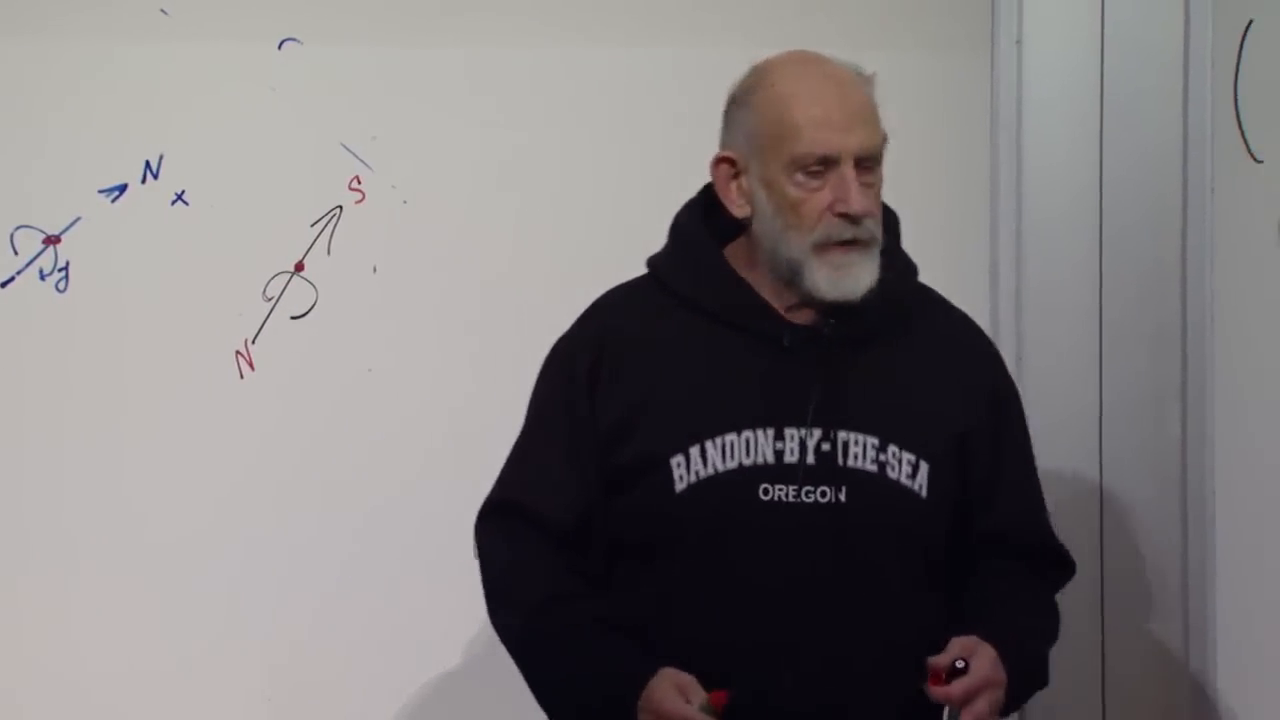
\includegraphics[width=0.94\linewidth]{lecture_08_frame_06.png}
\caption{時間反転の議論の際の、磁気軸と電荷変位の対になったスケッチ。上の簡潔なTikZ図は、部分的に消された生の黒板から変換内容を切り出したものである。}
\lectureframe{01:06:10}
\end{figure}

\begin{classroomqa}
\lecturetimestamp{01:06:38}
\audiencequestion{時間反転の下で、電流と電荷の両方が反転するのか。}
\lecturerresponse{電流は速度が反転するために反転する；電荷そのものは反転しない。電荷の符号を反転させるのは電荷共役\(C\)であり、時間反転\(T\)ではない。}
\end{classroomqa}

\begin{classroomqa}
\lecturetimestamp{01:07:01}
\audiencequestion{時間反転の反ユニタリ性は、非相対論的量子力学が時間反転不変でないことを意味するのか。}
\lecturerresponse{否。反ユニタリ性は、時間反転が量子力学において整合的に表現されるまさにその方法である：それは振幅を複素共役にし、運動量とスピンを反転させる。特定のハミルトニアンが不変であるかどうかは別の問題である。}
\end{classroomqa}

\begin{classroomqa}
\lecturetimestamp{01:07:19}
\audiencequestion{EDMの議論には、電子が点状ではなく有限の体積を持つことが必要か。}
\lecturerresponse{否。点粒子の有効ハミルトニアンは\(-d_e\,\widehat{\mathbf S}\!\cdot\!\mathbf E\)を含みうる。実験は、反対向きのスピン配向が異なる電場エネルギーを得るかどうかを問うのであり、文字通りの広がった電荷雲を分解する必要はない。}
\end{classroomqa}

パリティは弱い相互作用の対称性ではない；それはそれらのカイラル結合において可能な限り強く破れている。時間反転もまた厳密ではないが、標準模型における既知の破れが電子EDMに寄与するのは極めて小さなレベルにおいてのみである。非零の標準模型の寄与を計算することはできるが、それはここで議論した感度のはるかに下にある。したがって、ヌル結果は標準模型と整合しつつ、はるかに大きな時間反転の破れを生みうる拡張---例えば超対称性やその他の新しい相互作用---に切り込むものである。

基本的な実験的発想は単純である。磁場はスピンの向きを分裂させることによって磁気双極子を明らかにする。電場は、スピンに相関した追加のエネルギーシフトによってEDMを明らかにするであろう。実際の精密実験は、素朴な装置の中の孤立した電子ではなく、原子や分子、長いコヒーレント歳差時間、印加磁場の反転、そして系統誤差の注意深い制御を用いる。

\begin{classroomqa}
\lecturetimestamp{01:11:02}
\audiencequestion{EDM探索は高エネルギー衝突実験であったのか、それとも物質的な対象を用いた実験であったのか。}
\lecturerresponse{それは、制御された原子または分子環境に束縛された電子を、電場および磁場とともに用いる精密な卓上物理学であった。そのエネルギーは低いが、微小な対称性破れのシフトに対する感度は、高エネルギーの新物理学を間接的に探るものである。}
\end{classroomqa}

\begin{classroomqa}
\lecturetimestamp{01:12:21}
\audiencequestion{このヌル結果は、標準模型のどのような修正がなお実行可能であり続けるかを制約するのか。}
\lecturerresponse{原理的にはそうである。すべての模型は係数を予言し、したがって何らかのパラメータ領域を占める。詳細な数値的排除には専門家による計算が必要であるが、一般的な論理は堅固である---標準模型との一致がより高い精度で得られるほど、大きなEDMを予言する代替案の余地は小さくなる。}
\end{classroomqa}

\begin{classroomqa}
\lecturetimestamp{01:13:09}
\audiencequestion{量子情報の保存には時間反転対称性が必要か。}
\lecturerresponse{いいえ。ハミルトニアンが\(T\)の下で不変でなくても、ユニタリな時間発展は情報を保存する。固定された磁場中の粒子はよく知られた例である。その磁場は、磁場も同時に反転しない限り、時間反転した映画の中で一つの向きを選び出すが、それでも量子発展はユニタリのままである。局所ローレンツ不変量子場理論の通常の仮定の下では、\(CPT\)の結合変換は対称性であるが、それがユニタリ性を保証しているのではない。}
\end{classroomqa}

ここでこの中断を終えることができる。ヌル測定は、述べられた感度において電子に検出されたEDMが存在しないことを述べている。それは電子が球であるとは述べておらず、標準模型を覆すものでもない。それは、その模型からのいくつかの提案された逸脱を持続させることをより難しくする。

\section{第二量子化へ戻る：フーリエ変換、運動量モード、局所性}

我々は第二量子化を行っていた。通常の一粒子波動関数についてのよく知られた事実から穏やかに再開し、それを演算子へと持ち上げよう。フーリエ変換との関係は厳密かつ単純である。

\subsection{位置空間から運動量空間へ}

小文字の\(\psi\)であり、大文字の\(\Psi\)ではないものが、単一粒子の波動関数である。位置空間では、
\begin{equation}
P(x)=|\psi(x)|^2
\end{equation}
は粒子が位置\(x\)に見出される確率密度である。運動量空間の波動関数はそのフーリエ変換であり、
\begin{equation}
\tilde{\psi}(p)=\int dx\,\psi(x)\,\frac{e^{-ipx}}{\sqrt{2\pi}},
\end{equation}
であり、逆関係は
\begin{equation}
\psi(x)=\int dp\,\tilde{\psi}(p)\,\frac{e^{ipx}}{\sqrt{2\pi}}.
\end{equation}
である。このとき
\begin{equation}
P(p)=|\tilde{\psi}(p)|^2
\end{equation}
は運動量\(p\)に対する確率密度である。

我々は\(\hbar=1\)を用いる。二つの変換は逆変換の関係にある。すなわち、どちらか一方の波動関数を知れば他方が定まるが、それらの絶対値の二乗は異なる測定の問いに答える。

自由粒子に対しては、
\begin{equation}
H=\frac{p^2}{2m},
\end{equation}
であるから、運動量固有状態はエネルギー固有状態でもあり、その位置空間の波動関数は平面波である。
\begin{equation}
\psi_p(x)\propto e^{ipx}.
\end{equation}
これが第二量子化版への出発点である。

\begin{figure}[htbp]
\centering
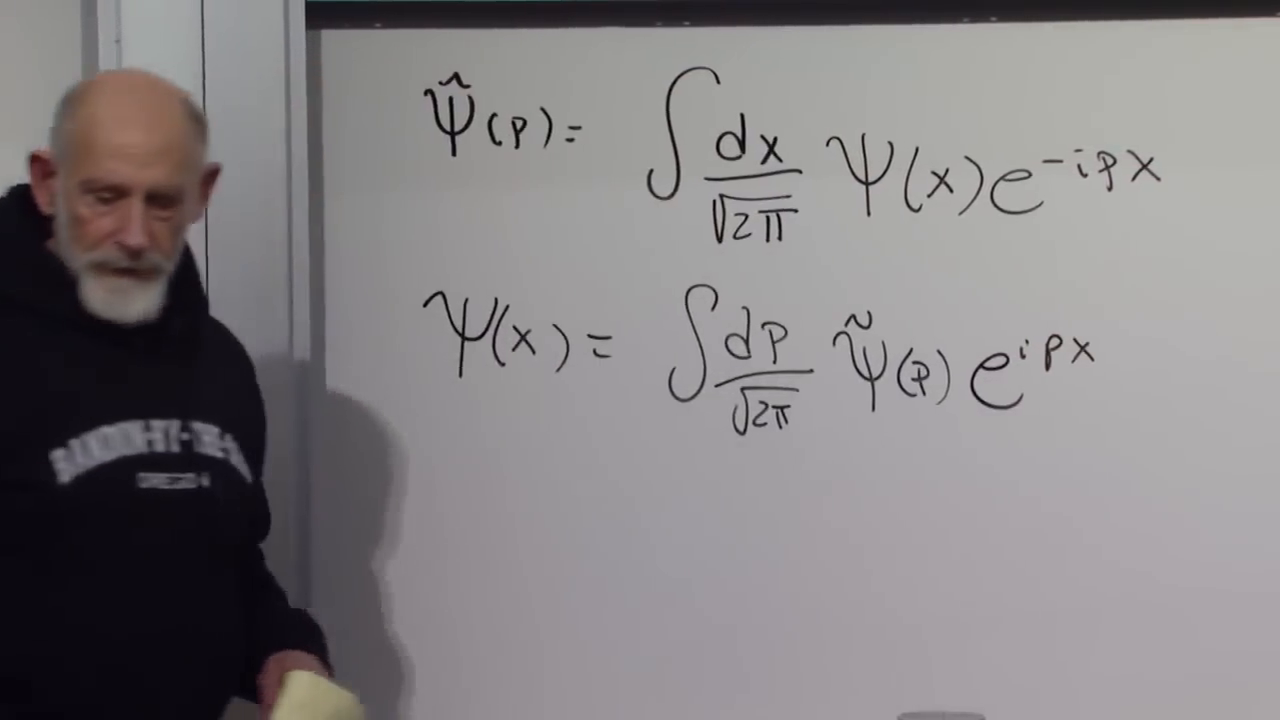
\includegraphics[width=0.94\linewidth]{lecture_08_frame_07.png}
\caption{一粒子波動関数に対する位置--運動量のフーリエ対。小文字の\(\psi\)と、次に導入される大文字の場の演算子との区別は本質的である。}
\lectureframe{01:20:00}
\end{figure}

\subsection{位置空間および運動量空間における場の演算子}

さて場の演算子に戻ろう。黒板ではその消滅部分と生成部分が\(\Psi_-(x)\)および\(\Psi_+(x)\)と書かれている。しばらくその記法を保つと、
\begin{align}
\Psi_-(x) &= \sum_i a_i\,\psi_i(x),\\
\Psi_+(x) &= \sum_i a_i^\dagger\,\psi_i^*(x).
\end{align}
ここで\(\psi_i(x)\)は\(i\)番目のモードの通常の一粒子波動関数であり、\(a_i\)と\(a_i^\dagger\)はそのモードの粒子を消滅および生成する。この時点から、次のように改名するのが便利である。
\[
\Psi(x)\equiv \Psi_-(x),
\qquad
\Psi^\dagger(x)\equiv \Psi_+(x).
\]

自由粒子に対しては、離散的なモードラベル\(i\)は連続的な運動量ラベル\(p\)に置き換えられる。平面波\(e^{ipx}\)を用いると、標準的な再構成された公式が得られる。
\begin{align}
\Psi(x) &= \int \frac{dp}{\sqrt{2\pi}}\,a(p)\,e^{ipx},\\
\Psi^\dagger(x) &= \int \frac{dp}{\sqrt{2\pi}}\,a^\dagger(p)\,e^{-ipx}.
\end{align}
これらは通常のフーリエ変換の場の演算子版である。それらは以前とまったく同様に厳密に逆変換できる。
\begin{align}
a(p) &= \int \frac{dx}{\sqrt{2\pi}}\,\Psi(x)\,e^{-ipx},\\
a^\dagger(p) &= \int \frac{dx}{\sqrt{2\pi}}\,\Psi^\dagger(x)\,e^{ipx}.
\end{align}
\(1/\sqrt{2\pi}\)の因子は、順変換と逆変換が同じ規格化をもつように選ばれた慣習である。

概念的な内容は単純である。\(\Psi^\dagger(x)\) は位置 \(x\) に粒子を生成し、\(a^\dagger(p)\) は運動量 \(p\) を持つ粒子を生成する。位置空間と運動量空間の生成演算子は互いにフーリエ共役であり、通常の量子力学において \(\psi(x)\) と \(\tilde{\psi}(p)\) がフーリエ共役であるのと同じである。

運動量 \(p\) の粒子が存在しなければ、\(a(p)\) はその状態を消滅させる。その運動量の粒子が存在すれば、通常の占有数係数とともに一つを除去する。同様に、\(\Psi(x)\) は \(x\) にある粒子を除去し、これは分布的あるいは波動束に塗り込んだ後に理解される。各粒子種はそれぞれ独自の場の演算子を必要とし、一つの場があらゆる種類の粒子を生成することはできない。

\subsection{ボソンの交換関係と離れた測定の独立性}

次の事実は定義から直接導出できる。ボソンに対して、
\begin{equation}
[a_i,a_j^\dagger]=\delta_{ij},
\qquad
[a_i,a_j]=0,
\qquad
[a_i^\dagger,a_j^\dagger]=0.
\end{equation}
連続版は
\begin{equation}
[a(p),a^\dagger(p')]=\delta(p-p').
\end{equation}
である。ここで離散展開から等時場の交換関係を計算する：
\begin{align}
[\Psi(x),\Psi^\dagger(y)]
&= \sum_{i,j}\psi_i(x)\psi_j^*(y)\,[a_i,a_j^\dagger] \\
&= \sum_i \psi_i(x)\psi_i^*(y) \\
&= \delta(x-y),
\end{align}
ここで最後のステップは一粒子基底の完全性を用いている。同様に、
\begin{equation}
[\Psi(x),\Psi(y)]=0,
\qquad
[\Psi^\dagger(x),\Psi^\dagger(y)]=0.
\end{equation}

\begin{figure}[htbp]
\centering
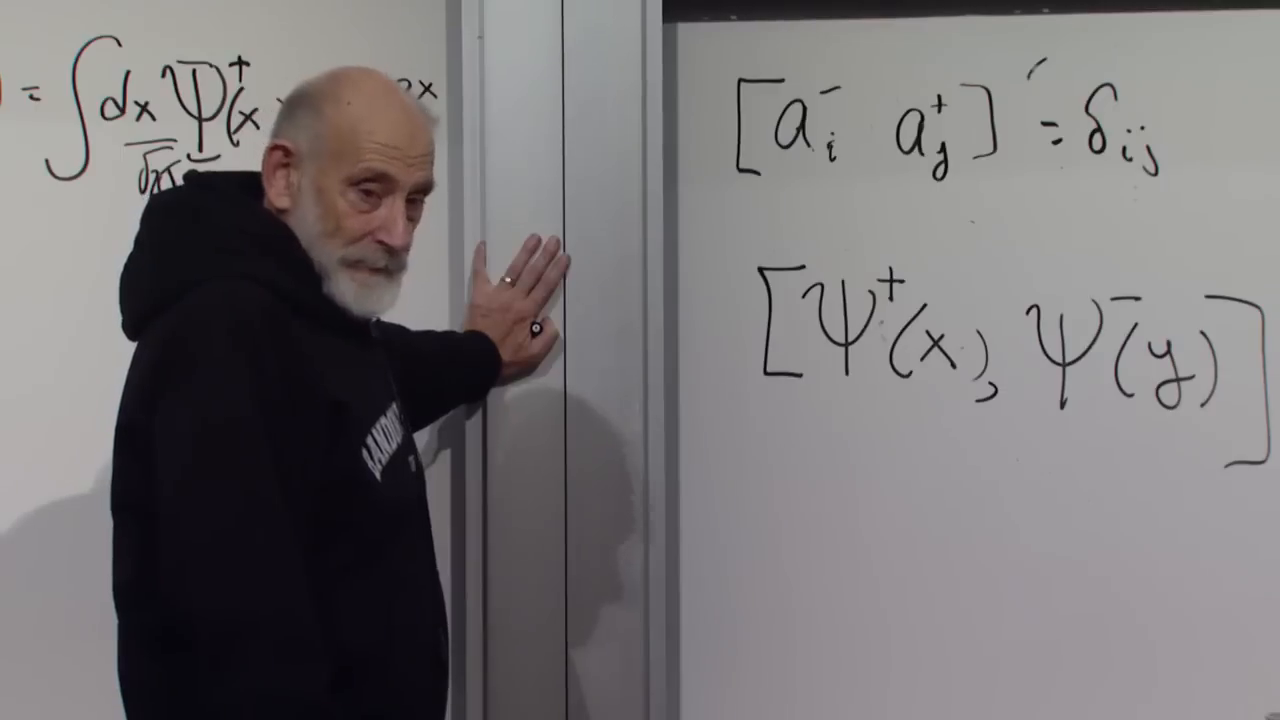
\includegraphics[width=0.94\linewidth]{lecture_08_frame_08.png}
\caption{モードの交換関係とその位置空間における対応物を黒板に示す。完全性により \(\delta_{ij}\) は空間的デルタ分布 \(\delta(x-y)\) になる。}
\lectureframe{01:31:00}
\end{figure}

重要な点は単に \(\Psi\) が非エルミートであることではない。エルミートな直交成分を定義する：
\begin{equation}
Q(x)=\frac{\Psi(x)+\Psi^\dagger(x)}{\sqrt{2}},
\qquad
P(x)=\frac{\Psi(x)-\Psi^\dagger(x)}{i\sqrt{2}}.
\end{equation}
それらの同一点における交換関係はデルタ分布を受け継ぐ。したがって、二つの局所直交成分は位置と運動量が共役であるのと同じ意味で共役である。一方を鋭くしようとすると他方に不確定性が生じる。

\begin{classroomqa}
\lecturetimestamp{01:32:03}
\audiencequestion{\(x=y\) のときデルタ関数は何を意味するのか。交換関係はどこでも大きいのか。}
\lecturerresponse{デルタは分布であり、有限の点値を持つ通常の関数ではない。引数が離れていれば消え、試験関数との積分の後にのみ有限の結果を与える。有限の検出器領域にわたり場を塗り込むと、形式的な同一点の特異性は二つのモードの通常の有限な正準交換関係になる。}
\end{classroomqa}

しかし \(x\neq y\) に対しては、等時交換関係は消える。二つの互いに素な領域に局在する操作は独立に実行できる：ここで場を測定しても、そこでの場に量子的なキックを与えない。これは相対論的微視的因果性の非相対論的な等時先駆である。相対論的理論では、物理的な局所可観測量は空間的隔たりで交換し、そこでは光信号が二つの事象を結ぶことができない。

非可換な可観測量との対比はよく知られている。\([x,p]=i\) であるから、精密な位置測定は運動量を乱し、精密な運動量状態は位置において広がる。異なるスピン成分が交換しないため、一つの成分を鋭く準備すると別の成分が不確定になる。離れた局所可観測量間の非零の交換関係は、同様に、一方の領域での操作が他方を乱すことを意味し、要求される因果的独立性と矛盾する。

\begin{classroomqa}
\lecturetimestamp{01:37:51}
\audiencequestion{EPR とエンタングルメントの実験は、ここでの測定が遠方の測定に影響を与えることを示すのか。}
\lecturerresponse{それらは相関を示すのであり、制御可能な因果的影響を示すのではない。エンタングルした結果は古典的因数分解を破るが、遠方の検出器における局所統計は、ここでの測定の選択や実行によって変えることはできない。空間的に離れた可観測量の交換関係は、そのノーシグナリング独立性の背後にある演算子としての言明である。}
\end{classroomqa}

次回は代数が変わる。フェルミオンの生成消滅演算子は反交換関係を満たす。素朴に考えると、離れた点におけるフェルミオン場は交換しないので、場自体を直接測定可能なボソン的可観測量として解釈することはできない。物理的なフェルミオン的可観測量は偶の組み合わせ---密度、電流、応力テンソル---であり、それらの局所可観測量は要求される空間的隔たりでの交換性を回復する。これが第二量子化のフェルミオン版への入口である。

\chapter{局所量子場と一次元ディラック方程式}

我々はすでに、量子場をその量子、生成消滅演算子、そして非相対論的粒子に対する最も単純なハミルトニアンを通して見てきた。ここではその仕組みを実際に働かせてみよう。まず、空間的に局所的なハミルトニアンがどのように運動量を保存するかを、単に主張するのではなく、実際に見る。次に、場の積が散乱と崩壊を記述することを見て、ハミルトニアンの繰り返し作用が図式的摂動論の初歩を生み出すのを眺める。その後になって初めて、約束したフェルミオンの問題に取り掛かる。最も明快な入口は、まだフェルミオン場ではなく、一次元ディラック方程式である。

\section{場のハミルトニアンをもう一度}

一種類の非相対論的粒子に対するハミルトニアンを次のように書く。
\begin{equation}
H_0=\int dx\,
\psi^\dagger(x)
\left[-\frac{\partial_x^2}{2m}+V(x)\right]
\psi(x).
\label{eq:l9-nonrel-hamiltonian}
\end{equation}
この記法は一次元に見えるが、冒頭の議論はその制限に依存しない。三次元では、\(x\)はベクトル\(\mathbf{x}\)を表し、\(dx\)は\(d^3x\)を、\(-\partial_x^2\)は\(-\nabla^2\)を表すことができる。

演算子\(\psi^\dagger(x)\)は\(x\)に粒子を生成し、\(\psi(x)\)はそこにある粒子を消滅させる。それらの正規順序積
\begin{equation}
n(x)=\psi^\dagger(x)\psi(x)
\end{equation}
は局所数密度である。したがってポテンシャル項は
\begin{equation}
H_V=\int dx\,V(x)n(x).
\end{equation}
と書ける。これはまさに古典気体に対して書くものと同じである。\(x\)の近くの粒子を数え、それぞれにポテンシャルエネルギー\(V(x)\)を割り当て、空間について足し合わせる。この段階では粒子は互いに相互作用しない。外部から課されたポテンシャルに応答することはあるが、それ以外にハミルトニアンは独立な一粒子エネルギーの和である。

単純化してから逆戻りするのが有用である。ポテンシャルを定数\(V(x)=V_0\)とする。定数ポテンシャルは力を及ぼさないが、その演算子としての意味は明白である。
\begin{equation}
\begin{aligned}
H_V&=V_0\int dx\,\psi^\dagger(x)\psi(x)=V_0N,\\
N&=\int dx\,n(x).
\end{aligned}
\end{equation}
これは各粒子に同じ付加エネルギーを与える。非相対論的記述で静止エネルギーを保つには、\(V_0=mc^2\)と選ぶ。するとこの項は粒子一つあたり静止エネルギー一つを数える。この他には退屈な定数を保持するのは、それが並進不変性を保ち、数え上げ操作を可視化するからである。

\section{更新規則としてのハミルトニアン}

運動量が保存されるとはどういうことか。その答えは、ハミルトニアンが何をするかという観点から述べるべきである。\(\psi\) を場の演算子、一粒子波動関数、多体状態のすべてに同時に使うことを避けるため、多体状態を \(\lvert\Phi(t)\rangle\) と呼ぶことにしよう。短い区間 \(\epsilon\) の間に、
\begin{equation}
\lvert\Phi(t+\epsilon)\rangle
=\left(1-i\epsilon H+O(\epsilon^2)\right)
\lvert\Phi(t)\rangle,
\label{eq:l9-short-update}
\end{equation}
ここで \(\hbar=1\) である。変化しない状態が第一項であり、最初の補正は \(H\) によって生成される。この更新を繰り返すことが Schr\"odinger 方程式である。

運動量保存は今や具体的な意味を持つ。初期状態が確定した全運動量\(P\)を持つならば、\(H\lvert\Phi\rangle\)も同じ全運動量を持たねばならない。他の性質は変化しうるし、個々の粒子は運動量を交換しうるが、ハミルトニアンが状態を異なる全\(P\)を持つセクターへ移すことはできない。これはハミルトニアンを運動量基底で書き直すことによって直接確かめられる。

\section{運動量のデルタ関数としての空間積分}

フーリエの規約を
\begin{align}
\psi(x)&=\int\frac{dp}{\sqrt{2\pi}}\,a(p)e^{ipx},\\
\psi^\dagger(x)&=\int\frac{dq}{\sqrt{2\pi}}\,a^\dagger(q)e^{-iqx}.
\label{eq:l9-field-fourier}
\end{align}
と選ぶ。演算子\(a(p)\)は運動量\(p\)の粒子を消滅させる。演算子\(a^\dagger(q)\)は運動量\(q\)の粒子を生成する。異なる文字を使うことが本質的である。二つの運動量は、空間積分がそれらを関係づけるまで独立に積分される。

数演算子の項から始める。
\begin{align}
N
&=\int dx\,\psi^\dagger(x)\psi(x)\\
&=\int\frac{dp\,dq}{2\pi}\,
a^\dagger(q)a(p)
\int dx\,e^{i(p-q)x}.
\end{align}
残りの積分は
\begin{equation}
\int dx\,e^{i(p-q)x}=2\pi\delta(p-q).
\end{equation}
である。\(p\ne q\)に対しては、位相が振動し、正と負の寄与の間で相殺される。\(p=q\)に対しては、まったく振動しない。ディラックのデルタ分布は、これら二つの事実を組み合わせる正確な対象である。したがって、
\begin{align}
N
&=\int dp\,dq\,a^\dagger(q)a(p)\delta(p-q)\\
&=\int dp\,a^\dagger(p)a(p).
\label{eq:l9-number-momentum}
\end{align}
この演算子は運動量\(p\)の粒子を取り除き、まったく同じ運動量の粒子を一つ戻す。決定的な要素は\(x\)に関する積分であった。それが、入る運動量と出る運動量の等しさを強制するデルタ関数を生み出した。

\begin{classroomqa}
\lecturetimestamp{00:17:02}
\audiencequestion{\(p=q\)のときに現れる無限大はどうなったのか。}
\lecturerresponse{デルタ関数はその高さを評価することによって使われるのではない。それは積分によって定義される分布である。\(\int dk\,\delta(k)f(k)=f(0)\)。「``無限に高く、無限に狭い''」という表現は、その積分された重みが1であることを思い出させるだけである。ここでは、\(p-q=0\)とせよと指示しており、無限の答えは残らない。}
\end{classroomqa}

同じ機構は、はるかに一般的な局所単項式に対しても働く。ある項がいくつかの消滅場といくつかの生成場を含み、それらが異なる種に属していてもよいが、すべて一点で評価され、その点について積分されるとしよう：
\begin{equation}
\int dx\,
\prod_{r=1}^{n} \psi_{i_r}^\dagger(x)
\prod_{s=1}^{m} \psi_{j_s}(x).
\end{equation}
消滅する粒子が運動量\(p_s\)を運び、生成される粒子が運動量\(q_r\)を運ぶとする。フーリエ展開により
\begin{equation}
\int dx\,
e^{i(\sum_s p_s-\sum_r q_r)x}
=2\pi\,
\delta\!\left(\sum_s p_s-\sum_r q_r\right).
\label{eq:l9-total-momentum-delta}
\end{equation}
が得られる。この結果は\(p_1\)を\(q_1\)と、\(p_2\)を\(q_2\)と、以下同様に、対にするのではない。それはただ
\begin{equation}
\sum_{\mathrm{annihilated}}p
=
\sum_{\mathrm{created}}q.
\end{equation}
を課すだけである。これはまさに相互作用に要求される規則である：個々の運動量は変化してよいが、全運動量は変化しない。より深い言明は並進不変性である。各点で同じ重みで積分された局所密度には特別な原点がなく、そのフーリエ変換は対応する運動量保存のデルタ関数を運ぶ。

\begin{classroomqa}
\lecturetimestamp{00:23:04}
\audiencequestion{提案されたハミルトニアン項は本当にこれらすべての場の演算子の積なのか。なぜそのような積を書くのか。}
\lecturerresponse{はい。この積は、どの粒子が一点で取り除かれ、どの粒子が生成されるかを指定する。その物理的動機は観測された散乱または崩壊過程から来るであろう。運動量の議論を先に確立しておくことで、それらの相互作用を直ちに読み取ることができる。}
\end{classroomqa}

\section{運動量空間と位置空間における運動エネルギー}

次に同じ仕組みを微分項に適用する。微分は平面波に作用する：
\begin{equation}
-\partial_x^2 e^{ipx}=p^2e^{ipx}.
\end{equation}
したがって
\begin{align}
H_{\mathrm{kin}}
&=\int dx\,\psi^\dagger(x)
\left(-\frac{\partial_x^2}{2m}\right)\psi(x)\\
&=\int dp\,\frac{p^2}{2m}\,a^\dagger(p)a(p).
\label{eq:l9-kinetic-momentum}
\end{align}
ここでも空間積分が入射運動量と出射運動量の等しさを強制する。新しい因子\(p^2/2m\)は、各運動量モードの粒子数をそのモードの運動エネルギーで重み付けするだけである。

\begin{classroomqa}
\lecturetimestamp{00:24:46}
\audiencequestion{平面波を二回微分すると負符号が付くべきか。}
\lecturerresponse{はい、\(\partial_x^2e^{ipx}=-p^2e^{ipx}\)。ハミルトニアンにはすでに補償する負符号が含まれているので、\(-\partial_x^2\)は正の固有値\(p^2\)を持つ。}
\end{classroomqa}

\begin{classroomqa}
\lecturetimestamp{00:27:20}
\audiencequestion{運動エネルギーが保存されるのはポテンシャルが定数のときだけか。}
\lecturerresponse{はい。位置に依存するポテンシャルがなければ力はなく、運動エネルギーは別個に保存される。非定数の外部ポテンシャルでは、全ハミルトニアンが陽に時間依存しなければ、運動エネルギーとポテンシャルエネルギーは交換し合いながら全ハミルトニアンは保存される。}
\end{classroomqa}

\begin{classroomqa}
\lecturetimestamp{00:27:42}
\audiencequestion{運動量空間の運動ハミルトニアンにおいて\(\psi^\dagger\psi\)の役割は何か。}
\lecturerresponse{それは数え上げ演算子である。モード積\(a^\dagger(p)a(p)\)は運動量\(p\)の粒子を数え、因子\(p^2/2m\)はそれぞれに適切な運動エネルギーを割り当てる。}
\end{classroomqa}

正値性を見る第二の方法がある。一度部分積分し、境界項を無視すると
\begin{align}
\int dx\,\psi^\dagger(-\partial_x^2)\psi
&=\int dx\,(\partial_x\psi^\dagger)(\partial_x\psi).
\label{eq:l9-positive-kinetic}
\end{align}
が得られる。無限遠で適切に消える場、または周期的境界条件では、境界からの寄与はゼロである。結果は絶対値の二乗の形をしており、非負である。それはまた場の理論に共通するパターンを示している：エネルギーは場の空間微分の二乗を含む。

\section{局所接触相互作用}

ここで場の積に物理的な仕事を与えよう。二つの種を考え、描像を親しみやすく保つためだけにそれらを電子と陽子と呼ぶ。当面それらは意図的に偽物である：どちらもボソン演算子で扱われ、それらの真のクーロン相互作用は省略される。それらの自由ハミルトニアンは
\begin{equation}
H_0=\int dx\left[
\psi_e^\dagger\left(-\frac{\partial_x^2}{2m_e}\right)\psi_e
+
\psi_p^\dagger\left(-\frac{\partial_x^2}{2m_p}\right)\psi_p
\right].
\end{equation}
モデル相互作用
\begin{equation}
H_{\mathrm{contact}}
=g\int dx\,
\psi_e^\dagger(x)\psi_p^\dagger(x)
\psi_e(x)\psi_p(x).
\label{eq:l9-contact}
\end{equation}
を加える。これを右から左へ読む。それは同じ点\(x\)にある電子と陽子を探し、それらを消滅させ、その点で両方を再生成する。二つの粒子が一緒になければ、この局所項はゼロを与える。それらの世界線が出会えば、全運動量を保存しながら個々の運動量を変えうる。したがってそれは理想化されたゼロ距離散乱ポテンシャルとして働く。

\begin{figure}[htbp]
\centering
\includegraphics[width=0.94\linewidth]{lecture_09_frame_02.png}
\caption{黒板上の接触相互作用。四つの局所場演算子が時空のスケッチの上に現れ、出会いの点が理想化された相互作用が作用する唯一の場所である。}
\lectureframe{00:35:36}
\end{figure}

\begin{figure}[htbp]
\centering
\begin{tikzpicture}[x=1.2cm,y=1.0cm,>=Latex]
\draw[->] (-3.0,0) -- (3.0,0) node[right] {$x$};
\draw[->] (0,-0.2) -- (0,4.2) node[above] {$t$};
\coordinate (v) at (0,2.0);
\fill (v) circle (1.8pt);
\draw[thick,->] (-2.2,0.4) -- (v);
\draw[thick,->] (2.0,0.4) -- (v);
\draw[thick,->] (v) -- (-1.6,3.7);
\draw[thick,->] (v) -- (2.2,3.7);
\node[left] at (-1.65,0.7) {$e$};
\node[right] at (1.55,0.7) {$p$};
\node[left] at (-1.15,3.3) {$e$};
\node[right] at (1.65,3.3) {$p$};
\node[right] at (0.12,2.05) {$g$};
\end{tikzpicture}
\caption{局所散乱描像の明快な再構成。頂点は式~\eqref{eq:l9-contact}の演算子の略記であり、古典的な衝突法則ではない。}
\end{figure}

実際の電子と陽子はクーロンポテンシャルを通じて遠隔的に相互作用する。接触モデルは最初の短い一歩にすぎない：もし実験が二つの種が重なるときにのみ散乱することを示すなら、式~\eqref{eq:l9-contact}はハミルトニアンに置くであろう種類の項である。

\begin{classroomqa}
\lecturetimestamp{00:35:40}
\audiencequestion{エネルギーが変化しないのなら、なぜこの散乱演算子はハミルトニアンの一部なのですか。}
\lecturerresponse{ハミルトニアンはエネルギー演算子であると同時に、状態を変化させる生成子でもある。二つの粒子間のポテンシャルエネルギーは、時間発展の下で散乱を引き起こす。全エネルギーの保存は、状態や粒子の個々の運動量が変わらないことを意味しない。}
\end{classroomqa}

これで実用的な規則が得られる。まず、粒子がどのような局所過程を経ることができるかを実験から学ぶ。次に、それらの過程を状態を更新する演算子に符号化する。場の積は装飾的な代数ではない。そのダガー付き因子とダガーなし因子が、どの種が現れ、どの種が消えるかを指定する。

\section{崩壊、逆過程、エルミート性}

泡箱が種\(A\)の飛跡を明らかにし、それが終わる点から飛跡\(B\)と\(C\)が現れるとしよう。局所過程は
\begin{equation}
A\longrightarrow B+C.
\end{equation}
であり、それを実行する演算子は
\begin{equation}
V=g\int dx\,
\psi_B^\dagger(x)\psi_C^\dagger(x)\psi_A(x).
\label{eq:l9-decay-half}
\end{equation}
である。消滅場が\(A\)を除去し、二つの生成場が同じ点で\(B\)と\(C\)を生成する。すべての\(x\)にわたって等しい重みで積分することは空間並進不変性を表し、直ちに
\begin{equation}
p_A=p_B+p_C.
\end{equation}
を与える。

ハミルトニアンはエルミートでなければならない。これが\(e^{-itH}\)をユニタリにし、全確率を保存する。式~\eqref{eq:l9-decay-half}はそれ自体ではエルミートではないので、その随伴を加えなければならない。
\begin{equation}
H_{\mathrm{int}}
=\int dx\left[
g\,\psi_B^\dagger\psi_C^\dagger\psi_A
+g^*\,\psi_A^\dagger\psi_C\psi_B
\right](x).
\label{eq:l9-hermitian-vertex}
\end{equation}
実結合定数\(g\)に対して、二つの係数は同じである。エルミート共役は、ダガー付き場とダガーなし場を交換するだけでなく、演算子の順序も逆にする。このボソン的玩具模型では、異なる種の場は可換であるため、その反転は追加の複雑さを引き起こさない。

第二項は逆過程
\begin{equation}
B+C\longrightarrow A.
\end{equation}
を実行する。したがって、崩壊を許す閉じたユニタリなハミルトニアンは、再結合振幅も含む。これは、選ばれた外部運動量のあらゆる組に対して両方向が起こることを約束するものではない。エネルギーやその他の保存則が、一方の方向を運動学的に到達不可能にするかもしれない。これは、演算子とその随伴の両方が力学に属することを述べている。

\begin{classroomqa}
\lecturetimestamp{00:42:48}
\audiencequestion{逆過程も許されるという規則に例外はあり得ますか。}
\lecturerresponse{エルミートな閉じた系のハミルトニアンのレベルでは、例外はない。随伴相互作用が必要である。特定の逆反応は依然として運動学や別の保存量子数によって遮断され得るが、共役行列要素は存在する。}
\end{classroomqa}

数\(g\)は結合定数である。\(g\)が小さければ、出会った粒子は弱くしか相互作用しない。大きければ、遷移振幅はより大きい。結合定数は通常、実験で測定されるパラメータであるが、対称性が一見異なるいくつかの結合定数を関係づけることもある。

同じ文法がより複雑な反応も扱う。ベータ崩壊では、
\begin{equation}
n\longrightarrow p+e^-+\bar\nu_e,
\end{equation}
模式的な局所項は四つの場を含む。一つは中性子を消滅させ、三つは陽子、電子、電子反ニュートリノを生成し、さらにエルミート共役な過程も含む。これで、少数の演算子単項式がどのように量子場の理論を定義し始めるかを見るのに十分である。

\section{なぜハミルトニアンの二乗が重要か}

短時間の公式\eqref{eq:l9-short-update}は\(\epsilon\)の一次までしか保っていなかった。完全な展開は
\begin{equation}
e^{-i\epsilon H}
=1-i\epsilon H-\frac{\epsilon^2}{2}H^2
+\frac{i\epsilon^3}{3!}H^3+\cdots.
\label{eq:l9-exponential}
\end{equation}
である。二次ではハミルトニアンが二度作用する。これが最初の複合過程の図の代数的起源である。

頂点\(A\leftrightarrow B+C\)に対して、一回の作用で\(B+C\)を\(A\)に結合でき、二回目の作用でその\(A\)を再び\(B+C\)に分けることができる。
\begin{equation}
B+C\longrightarrow A\longrightarrow B+C.
\label{eq:l9-bc-scattering}
\end{equation}
正味の寄与は\(B+C\to B+C\)散乱振幅である。中間\(A\)は追加の観測事象ではなく、相互作用の二回の作用の間に和をとられる状態を表す。

\begin{classroomqa}
\lecturetimestamp{00:49:54}
\audiencequestion{書き下された二次の積において\(C\)場はダガーを持つべきですか。}
\lecturerresponse{はい、演算子の順序は述べられた順序と一致しなければならない。第一の頂点は\(B\)と\(C\)を消滅させ、\(A\)を生成する。第二の頂点は\(A\)を消滅させ、\(B\)と\(C\)を再生成する。対応するダガーを正しく書くことで、その解釈が回復される。}
\end{classroomqa}

\begin{figure}[htbp]
\centering
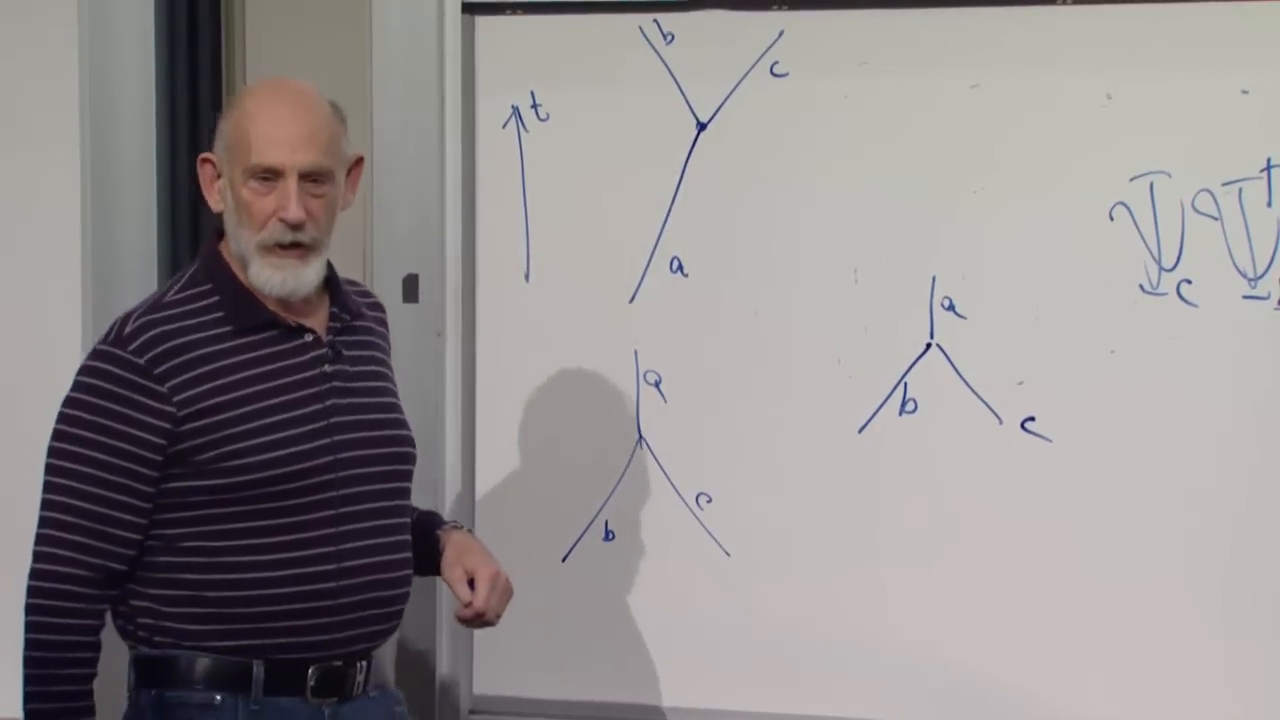
\includegraphics[width=0.94\linewidth]{lecture_09_frame_05.png}
\caption{黒板上の基本\(A\leftrightarrow B+C\)頂点の二つの向き。それらを並置することが、式~\eqref{eq:l9-bc-scattering}の二次過程の視覚的略記である。}
\lectureframe{00:48:56}
\end{figure}

ここで spectator \(B\) を追加する。1つの作用により \(A\) が \(C\) を放出して \(B\) になり、後の作用によりその \(C\) が元の \(B\) と結合して \(A\) を形成する。外部粒子は再び \(A+B\) であるが、それらの運動量は変化しうる。これを \(A\) と \(B\) の \(C\) の交換による散乱と呼ぶ。

\begin{figure}[htbp]
\centering
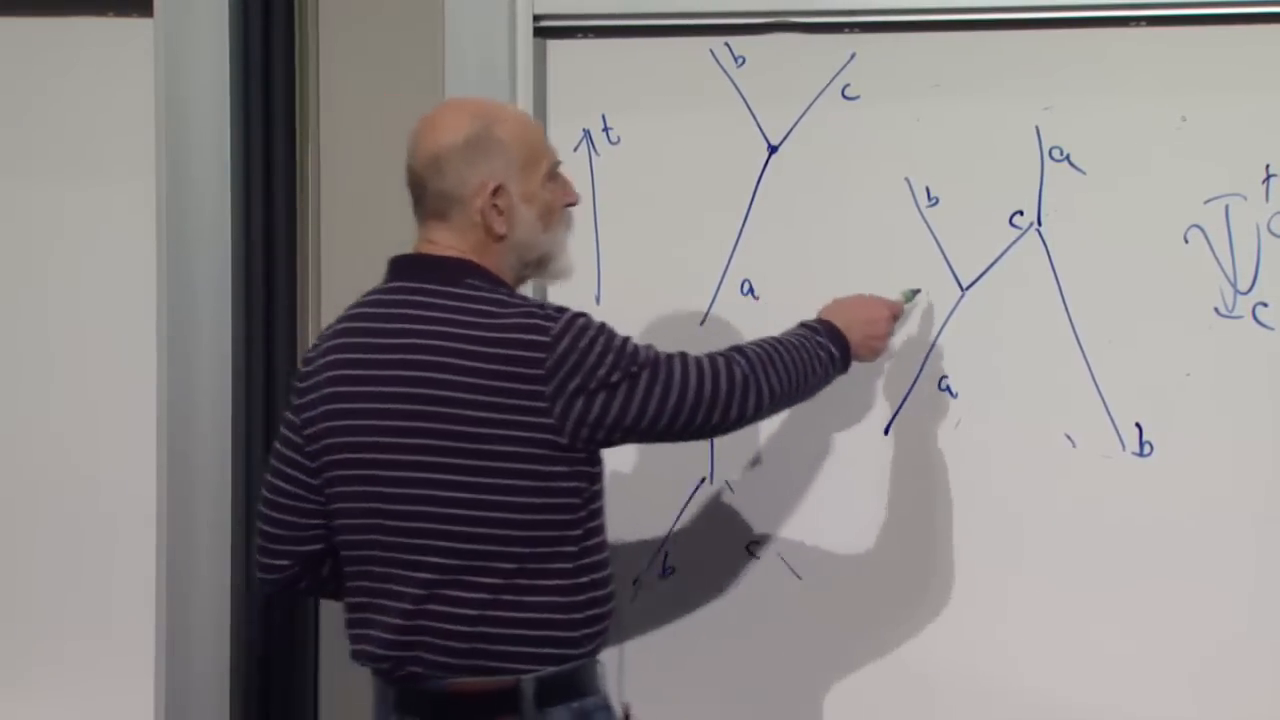
\includegraphics[width=0.94\linewidth]{lecture_09_frame_06.png}
\caption{黒板上の交換構成。右側の図は2つの素過程の頂点を内部 \(C\) 線で結び、外部の \(A\) 粒子と \(B\) 粒子が散乱する。}
\lectureframe{00:51:22}
\end{figure}

\begin{figure}[htbp]
\centering
\begin{tikzpicture}[x=1.1cm,y=1cm,>=Latex]
\draw[->] (-3.7,-0.2) -- (-3.7,4.2) node[above] {$t$};
\coordinate (v1) at (-0.9,1.25);
\coordinate (v2) at (0.9,2.95);
\fill (v1) circle (1.7pt);
\fill (v2) circle (1.7pt);
\draw[thick,->] (-2.6,0.2) -- (v1) node[midway,below left] {$A$};
\draw[thick,->] (2.6,0.2) -- (v2) node[midway,below right] {$B$};
\draw[thick,->] (v1) -- (-2.4,4.0) node[midway,left] {$B$};
\draw[thick,->] (v2) -- (2.5,4.0) node[midway,right] {$A$};
\draw[thick,->,dashed] (v1) -- (v2) node[midway,above left] {$C$};
\node[below] at (0,-0.05) {$A+B\rightarrow A+B$};
\end{tikzpicture}
\caption{\(C\) 交換の明快な再構成。各点は \(g\) の因子を一つ寄与するので、この二次の項は \(g^2\) に比例する。}
\end{figure}

各局所相互作用点を頂点と呼ぶ。各頂点はその結合定数の因子を寄与するので、二頂点の寄与は \(g^2\) を、三頂点の寄与は \(g^3\) を、以下同様に伴う。したがってハミルトニアンの一つの項は反応の大きな族を関連づける。この経済性は量子場の理論がこれほど強力である一つの理由である。少数の局所相互作用が膨大な散乱データを組織する。

\begin{classroomqa}
\lecturetimestamp{00:53:14}
\audiencequestion{過程 \(A\to B+C\to A\) を何と呼ぶか。}
\lecturerresponse{それは自己エネルギー寄与である。測定される \(A\) は裸の1粒子基底状態にすぎないのではない。相互作用する状態は近傍の \(B+C\) 成分の振幅も持つ。それからの散乱はその dressed 構造を明らかにしうる。}
\end{classroomqa}

量子電磁力学がよく知られた例を与える。局所的な電子--光子頂点は電子を消滅させ、電子を再生成し、光子を生成することができる。二次では、電子は光子を放出して再吸収してもよい。これを小さな映画のように語りたくなるが、その規律ある意味は摂動展開における一つの項である。物理的電子は光子を含む成分をもつ dressed 状態である。

この成分が ``約1パーセント'' であるという教室での見積もりは、微細構造定数 \(\alpha_{\mathrm{em}}\simeq 1/137\) が定める尺度を伝える。光子 Fock 成分の正確な確率はエネルギー分解能と相互作用状態の定義に依存し、孤立電子の普遍的な1パーセントの性質ではない。堅牢な主張は、相互作用が電子の測定可能な構造を変えるということである。

\section{図が語ることと語らないこと}

図は相互作用ハミルトニアンの冪のための計算上の略記である。それらは粒子が確実に1つの事象を行い、次に別の事象を行うという信頼できる古典的履歴ではない。どの中間的選択肢 ``が実際に起こったか'' を決めようと内部を覗くことは、通常の量子干渉と同様に、実験を変え、コヒーレントな和を破壊する。

\begin{classroomqa}
\lecturetimestamp{00:56:52}
\audiencequestion{最初の頂点でエネルギーと運動量の両方が保存されるか。}
\lecturerresponse{ここで行った等時刻ハミルトニアン構成では、空間積分は直ちに運動量デルタ関数を生じる。その孤立した挿入に対して時間積分はまだエネルギーデルタ関数を生じていない。完全な時間並進不変散乱振幅は全エネルギーを保存するが、中間線は観測粒子のオンシェル関係に従う必要はない。共変的図の言語では各頂点で4元運動量が保存されるが、内部粒子はオフシェルでありうる。}
\end{classroomqa}

素朴な頂点描像における見かけのエネルギー欠損は、相互作用エネルギーを捨ててはならないというもう一つの警告である。全ハミルトニアンは自由粒子エネルギーの和以上のものである。混乱が生じたなら、式~\eqref{eq:l9-exponential}に戻れ。この描像はユニタリ時間発展の展開における一つの項を表している。完全なファインマン図の技術は系統的な時間順序、伝播関数、積分、対称因子を与えるが、基本的な物理はここから始まる。

ある拡張された質問は、放出された光子をゆっくり動く電子の周囲の電場と比較することにより、図をあまりに文字通りに押しすぎている。

\begin{classroomqa}
\lecturetimestamp{00:58:26}
\audiencequestion{電子の距離における電場は、文字通り放射された光子によって生成されるのか。それは干渉やアハラノフ--ボーム効果とどう整合するのか。}
\lecturerresponse{静的場または誘導場は、実光子の流れではない。量子電磁力学は放射と電子の電磁的 dressing の両方を同じ場で記述するが、対応する量子状態と運動学は異なる。超相対論的電子では、一部の場の成分はほぼ実光子の流れのように有用に振る舞うことができる。遅い電子では、文字通りの光子の軌跡は誤ったモデルである。二重スリット干渉とアハラノフ--ボーム効果もまた非古典的な場の現象であるが、それらはこの自己エネルギー図を機械的な映画に変えるものではない。}
\end{classroomqa}

\begin{classroomqa}
\lecturetimestamp{01:01:28}
\audiencequestion{なぜ図の古典的モデルは正確には失敗するのか。}
\lecturerresponse{計算は許されたすべての中間選択肢からの振幅をコヒーレントに加えるからである。経験は図を直観的にするが、その文字通りの内容はそれを定義する演算子展開を決して超えない。それらは \(H^2,H^3,\ldots\) を計算するための簡潔な方法であり、観測された中間事象の記録ではない。}
\end{classroomqa}

\begin{classroomqa}
\lecturetimestamp{01:03:04}
\audiencequestion{通常のクーロン相互作用は光子交換の古典的極限として現れうるか。}
\lecturerresponse{はい。適切な光子媒介振幅を評価し、非相対論的静的極限を取るとクーロンポテンシャルが得られる。その導出は現在の演算子の概略よりも技術的であり、それでもなお光子が文字通り2つの古典的粒子の間を跳ぶものとして読まれるべきではない。}
\end{classroomqa}

\begin{classroomqa}
\lecturetimestamp{01:03:44}
\audiencequestion{結合定数は場の積から計算されるのか。}
\lecturerresponse{通常、それらの数値は実験的入力である。対称性はそれらを制約したり、そうでなければ独立であろう結合を関係づけたりすることができる。そのような関係が異なる反応の相対的強度を予測し、実験がそれを確認するとき、一致は特に有益である。}
\end{classroomqa}

\begin{classroomqa}
\lecturetimestamp{01:04:48}
\audiencequestion{偶発的対称性はゲージ対称性と比べてどのような役割を果たすのか。}
\lecturerresponse{ゲージ対称性は許される構造と結合間の関係を直接制約する。偶発的対称性は基礎的レベルで課されるものではないが、すべての低次で許される相互作用がたまたまそれを尊重するために現れる。それは依然として重要な帰結を持ちうるが、その起源と頑健性はゲージ対称性のそれとは異なる。}
\end{classroomqa}

非相対論的場の理論は今のところこれで十分である。我々はフェルミオンを約束した。それらを直ちに第二量子化するのではなく、まずそれらの場の演算子が満たさなければならない相対論的一粒子方程式を理解しよう。

\section{なぜ電子は相対論を必要とするのか}

まず一次元空間から始める。これは現実的な制限ではないが、三次元スピンの幾何学的複雑さを取り除きつつ、本質的な代数を保つことができる。電子は軽いので、原子の中でも相対論が重要になる。水素中でのその特徴的な速度は
\begin{equation}
v\sim\alpha_{\mathrm{em}}c\approx 0.007c,
\end{equation}
の程度であり、光速のおよそ1パーセントである。重い原子の内殻電子では、その粗い目安は \(v\sim Z\alpha_{\mathrm{em}}c\) となるので、相対論的補正はかなり大きくなりうる。歴史的な興味が決定的な動機であったか、原子の精度がそうであったかに関わらず、相対論的な Schr\"odinger 型方程式は物理的に必要である。

通常の量子化レシピはエネルギーと運動量の古典的関係から始まる。非相対論的には、
\begin{equation}
E=\frac{p^2}{2m},
\end{equation}
であり、置換
\begin{equation}
E\mapsto i\partial_t,
\qquad
p\mapsto-i\partial_x
\end{equation}
により
\begin{equation}
i\partial_t\varphi(x,t)
=-\frac{1}{2m}\partial_x^2\varphi(x,t).
\end{equation}
が得られる。

相対論では代わりに、\(c=1\) として、
\begin{equation}
E^2=p^2+m^2.
\label{eq:l9-rel-dispersion}
\end{equation}
が与えられる。

\begin{figure}[htbp]
\centering
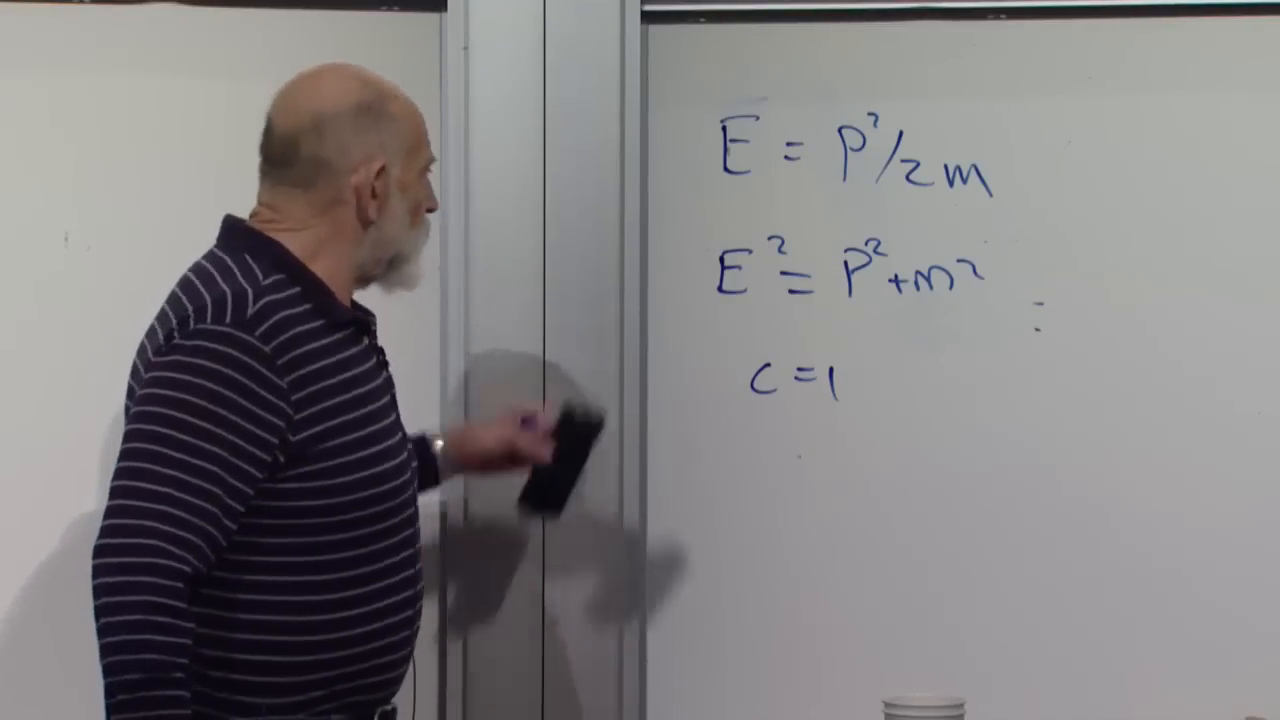
\includegraphics[width=0.94\linewidth]{lecture_09_frame_07.png}
\caption{黒板は \(E=p^2/2m\) から相対論的関係 \(E^2=p^2+m^2\) へ、\(c=1\) として移行する。}
\lectureframe{01:10:30}
\end{figure}

この置き換えを二乗した関係に適用すると
\begin{equation}
-\partial_t^2\varphi
=\left(-\partial_x^2+m^2\right)\varphi,
\label{eq:l9-klein-gordon}
\end{equation}
あるいは等価に
\begin{equation}
\left(\partial_t^2-\partial_x^2+m^2\right)\varphi=0.
\end{equation}
が得られる。これがKlein--Gordon方程式である。これは完全に意味のある相対論的場の方程式であり、特にスピンゼロの場に対してそうである。しかし、求めている電子の方程式は時間について一階でなければならない。
\begin{equation}
i\partial_t\Psi=H\Psi,
\end{equation}
すなわち、\(H^2\)だけでなく\(H\)自体が時間発展を生成するのである。

形式的に
\begin{equation}
H=\sqrt{-\partial_x^2+m^2}.
\end{equation}
を選ぶこともできよう。この平方根は運動量空間ではきれいに定義でき、そこでは\(\sqrt{p^2+m^2}\)を掛けることになるが、位置空間では非局所的な擬微分作用素である。それは技術的には意味があるものの、我々が求める局所方程式にとっては美的に役立たない。したがって、我々は再び出発する。

\section{質量ゼロの右進行波}

まず右へ進む質量ゼロの粒子を考える。その正エネルギーと運動量は
\begin{equation}
E=p
\qquad (c=1).
\end{equation}
を満たす。量子化すると
\begin{equation}
i\partial_t\psi=-i\partial_x\psi,
\end{equation}
または
\begin{equation}
(\partial_t+\partial_x)\psi=0.
\label{eq:l9-right-mover}
\end{equation}
となる。すべての解は
\begin{equation}
\psi(x,t)=f(x-t).
\end{equation}
の形をとる。その波形は剛直であり、光速で右へ進む。

直ちに二つの困難が現れる。第一に、式~\eqref{eq:l9-right-mover}を任意のフーリエモードに作用させると、負の運動量はエネルギー\(E=p<0\)をもつので、ハミルトニアンには下界がない。手で\(p>0\)に制限すれば右進行成分だけが残るが、それはまだ我々が望む電子の理論ではない。第二に、この方程式は一方通行であり、通常の左進行電子を含まない。我々はまず左右の問題を治し、負エネルギーの問題は露呈したままにしておく。

\section{二成分とアルファ行列}

二つの振幅を導入する。
\begin{equation}
\Psi(x,t)=
\begin{pmatrix}
\psi_1(x,t)\\[3pt]
\psi_2(x,t)
\end{pmatrix},
\end{equation}
ここで\(\psi_1\)は質量ゼロ極限で右進行、\(\psi_2\)は左進行である：
\begin{align}
(\partial_t+\partial_x)\psi_1&=0,
&
(\partial_t-\partial_x)\psi_2&=0.
\end{align}
量子力学ではまた、この二つの任意の重ね合わせも許される。したがって粒子は、一度きりで選ばれる古典的なラベルをもつのではなく、両方向に対する振幅をもちうる。

この余分な二値自由度は代数的にはスピンに似ているが、一次元では通常の角運動量ではない。
\begin{equation}
\alpha=
\begin{pmatrix}
1&0\\
0&-1
\end{pmatrix}
=\sigma_3.
\label{eq:l9-alpha}
\end{equation}
を定義する。その\(+1\)固有ベクトルは右進行成分を選び、\(-1\)固有ベクトルは左進行成分を選ぶ。質量ゼロの理論では、ハミルトニアンは単に
\begin{equation}
H=\alpha p,
\end{equation}
であり、二つの方程式は
\begin{equation}
i\partial_t\Psi=-i\alpha\partial_x\Psi.
\label{eq:l9-massless-dirac}
\end{equation}
にまとめられる。

\begin{classroomqa}
\lecturetimestamp{01:22:44}
\audiencequestion{二つの成分を区別する対角行列の名前は何か。}
\lecturerresponse{パウリ行列としては\(\sigma_3\)であり、\(\sigma_1\)ではない。現在の構成に対するディラックの記法では、これを\(\alpha\)と呼ぶ。その代数はよく知られたパウリ代数であるが、ここでの物理的ラベルはスピン角運動量ではなく方向である。}
\end{classroomqa}

\begin{classroomqa}
\lecturetimestamp{01:23:32}
\audiencequestion{方向がベクトルである三次元では、この構成はより幾何学的な意味をもつようになるのか。}
\lecturerresponse{はい。三次元の問題では各空間方向に対して一つの行列が必要となり、より豊かなスピノル構造へと導かれる。それでも一次元模型はそれ自身の設定において厳密であり、余分な複雑さなしに本質的な左右の代数を切り出している。}
\end{classroomqa}

\begin{figure}[htbp]
\centering
\includegraphics[width=0.94\linewidth]{lecture_09_frame_03.png}
\caption{黒板上の質量ゼロ二成分方程式：\(H=\alpha P\)。ここで対角行列は\(\psi_1\)と\(\psi_2\)に反対向きの伝播を割り当てる。}
\lectureframe{01:26:00}
\end{figure}

一方通行の問題は消えた。負エネルギーのスペクトルは残り、さらに第三の欠陥を発見した。すなわち、二つの成分は依然として質量ゼロで光速で伝播する。次の段階では静止エネルギーを導入し、方向を結合しなければならない。

\section{質量の追加とディラック代数の発見}

質量に比例する最も一般的な単純項を加える。
\begin{equation}
H=\alpha p+\beta m,
\label{eq:l9-dirac-hamiltonian}
\end{equation}
ここで\(\beta\)は二成分指数にのみ作用する。それは単位行列でも他の何らかの行列でもありえたが、相対論的分散関係に決定させる。

\(H^2\)が\(p^2+m^2\)に等しくなければならないので、式~\eqref{eq:l9-dirac-hamiltonian}を二乗する：
\begin{align}
H^2
&=(\alpha p+\beta m)^2\\
&=\alpha^2p^2+\beta^2m^2
+(\alpha\beta+\beta\alpha)pm.
\label{eq:l9-square-dirac}
\end{align}
これらの行列は\(p\)と可換である。なぜなら、それらは内部二成分空間に作用し、\(p\)は空間波動関数に作用するからである。式~\eqref{eq:l9-rel-dispersion}と一致させるには
\begin{equation}
\alpha^2=\mathbb{1},
\qquad
\beta^2=\mathbb{1},
\qquad
\{\alpha,\beta\}
=\alpha\beta+\beta\alpha=0.
\label{eq:l9-dirac-algebra}
\end{equation}
が必要である。第一の条件は\(\alpha=\sigma_3\)に対してすでに成り立つ。それとは異なるパウリ行列は、いずれもそれと反可換であり、二乗すると単位行列になる。ここでは次のように選ぶ。
\begin{equation}
\beta=
\begin{pmatrix}
0&1\\
1&0
\end{pmatrix}
=\sigma_1.
\label{eq:l9-beta}
\end{equation}
\(\sigma_2\)ではなく\(\sigma_1\)を選ぶのは基底の規約であり、どちらもユニタリな基底変換の後で同じ代数を実現する。

\begin{classroomqa}
\lecturetimestamp{01:33:00}
\audiencequestion{ディラックは、パウリ行列がこれらの代数的条件を満たすことを単に認識したのか。}
\lecturerresponse{歴史的な導出は三次元で直接行われ、必要な関係を満たす行列が導入された。条件を書き下してしまえば、パウリ代数によって一次元の解は直ちに得られる。すなわち、二つの異なるパウリ行列を選べばよい。}
\end{classroomqa}

\begin{classroomqa}
\lecturetimestamp{01:34:24}
\audiencequestion{この\(\beta\)は相対論的速度パラメータ\(v/c\)か。}
\lecturerresponse{いいえ。それはスピノル成分に作用する行列である。文字が再利用されているのはディラックの記法にすぎず、運動学的量\(v/c\)とは何の関係もない。}
\end{classroomqa}

3次元空間では、\(2\times2\)行列だけでは、必要とされる反交換行列の完全な組には不十分である。その拡張は後回しにする。1次元では、式~\eqref{eq:l9-alpha}と\eqref{eq:l9-beta}で十分である。

\section{結合した1次元ディラック方程式}

\(p=-i\partial_x\)を代入すると、ハミルトニアン形式の1次元ディラック方程式が得られる：
\begin{equation}
i\partial_t\Psi
=\left(-i\alpha\partial_x+\beta m\right)\Psi.
\label{eq:l9-one-dimensional-dirac}
\end{equation}
\(\alpha\)は対角であるから、その微分項は2つの成分を分離したまま保つ。\(\beta\)は非対角であるから、質量項はそれらを交換する。成分ごとに書くと、
\begin{align}
i\partial_t\psi_1
&=-i\partial_x\psi_1+m\psi_2,
\label{eq:l9-dirac-component-one}\\
i\partial_t\psi_2
&=+i\partial_x\psi_2+m\psi_1.
\label{eq:l9-dirac-component-two}
\end{align}

\begin{figure}[htbp]
\centering
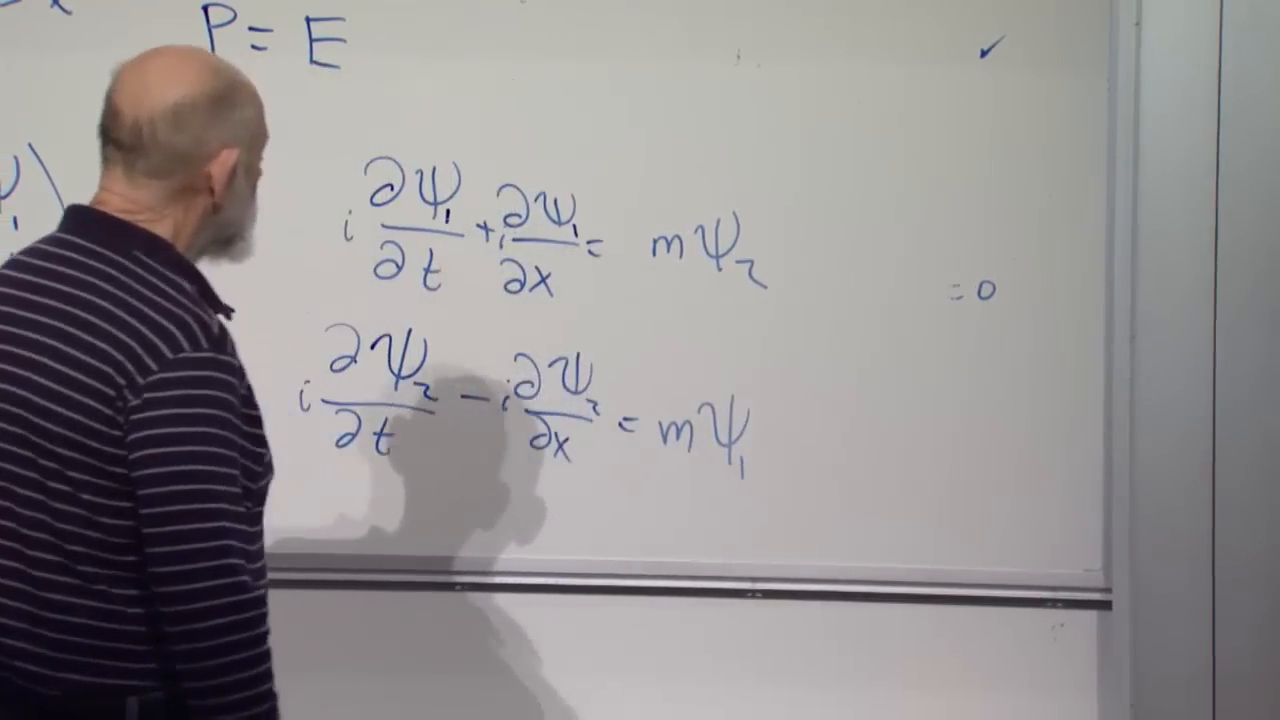
\includegraphics[width=0.94\linewidth]{lecture_09_frame_08.png}
\caption{黒板に書かれた結合成分方程式。逆符号の微分は右向きと左向きの運動を表し、非対角の質量項は\(\psi_1\)と\(\psi_2\)を入れ替える。}
\lectureframe{01:37:44}
\end{figure}

\(m\ne0\) になるとすぐに、成分は独立に発展しなくなる。一次方程式を二乗すると、各成分に対してクライン--ゴルドン演算子が回復され、
\begin{equation}
\left(\partial_t^2-\partial_x^2+m^2\right)\psi_a=0,
\qquad a=1,2,
\end{equation}
となり、平面波は \(E^2=p^2+m^2\) を満たす。その群速度は
\begin{equation}
v_g=\frac{dE}{dp}=\frac{p}{E},
\end{equation}
であり、その大きさは非零の質量に対して1未満である。

質量と左右混合の関係は偶然ではない。質量のない右向きの運動子は、任意の固有ローレンツブーストの下で右向きの運動子のままである。光速未満の観測者は光を追い越してその向きを逆にすることはできない。質量のある粒子は静止させることができ、次に同じ向きに動くより速い系から見ると、その速度は逆向きに見える。したがって、質量のある相対論的理論は右と左のセクターを永久に孤立させておくことはできない。非対角の質量項は、まさに必要な結合を与える。

\begin{classroomqa}
\lecturetimestamp{01:40:01}
\audiencequestion{2つの成分の入れ替わりはカイラル振動なのか？}
\lecturerresponse{この1次元基底では、\(\alpha\)が2つの質量のないカイラル方向を区別する。質量項は非対角であり、それらを混合するので、カイラリティはもはや保存されない。その意味で、質量項はカイラル振動の源である。}
\end{classroomqa}

\begin{classroomqa}
\lecturetimestamp{01:40:46}
\audiencequestion{なぜフェルミオンの方程式がボソンの方程式の平方根であるべきなのか？}
\lecturerresponse{そのように理解すべきではない。分散関係\(E^2=p^2+m^2\)は、統計に関係なく、すべての自由相対論的粒子に当てはまる。ディラック演算子はたまたまクライン--ゴルドン演算子の行列因子分解を与えるが、その代数的関係はフェルミオンをボソンから導くものではない。}
\end{classroomqa}

\begin{classroomqa}
\lecturetimestamp{01:41:31}
\audiencequestion{方程式は、左向きと右向きの因子への単純なスカラー因子分解に還元できるか？}
\lecturerresponse{質量のない極限でのみ、2つのカイラル方程式は独立なスカラー因子に分離する。\(m\ne0\)に対して、有用な因子分解は行列値的である：望まない交差項を取り除くのは、反交換する\(\alpha\)行列と\(\beta\)行列である。}
\end{classroomqa}

\begin{classroomqa}
\lecturetimestamp{01:42:04}
\audiencequestion{これら2つの結合方程式はすでにディラック方程式を構成しているのか？}
\lecturerresponse{はい。それらを合わせると1次元空間におけるディラック方程式であり、式~\eqref{eq:l9-one-dimensional-dirac}のコンパクトな形で等価に書ける。\(\beta\)を掛けることにより、より対称な共変的表記が得られるが、その形は後回しにする。}
\end{classroomqa}

2つの課題が意図的に未完成のまま残されている。この構成は負エネルギーを取り除いてはいない。それは両方の方向セクターに負エネルギー解を与えたので、その問題は今やより少なくではなく、より可視的になっている。そして理論は依然として1次元空間に住んでいる。負エネルギー解を解釈することと、行列代数を\(3+1\)次元に拡張することが次の段階である。

\chapter{フェルミオン、ディラック行列、ディラックの海}

ディラックの海が我々の目的地であるが、そこへの道筋が重要である。相対論的電子論における負エネルギーに直面する前に、二つの道具立てが必要である。まず、フェルミオンをボソンから区別する演算子代数が来る。次に、一次元ディラック方程式の復習が来る。そこでは、波動関数のあらゆる拡大が、三次元空間の幾何学なしに見て取れる。これらの道具立てが揃えば、三次元方程式が自らの行列構造を強いることになり、充填されたフェルミオン状態と空のフェルミオン状態についての冒頭の議論が、陽電子への鍵として戻ってくる。

我々は\(c=\hbar=1\)を用いる。大文字の\(P\)は運動量演算子を表し、小文字の\(p\)は運動量固有値を表し、太字の記号はそれらの三次元版を表す。

\section{交換は演算子代数となる}

二つの同種粒子を考え、一方が\(x\)に、他方が\(y\)にあるとする。ラベル\(x\)と\(y\)は完全な位置を表し、単一粒子の二つのデカルト座標ではない。二つの生成演算子を真空に作用させると
\begin{equation}
\lvert x,y\rangle
=
\psi^\dagger(x)\psi^\dagger(y)\lvert0\rangle.
\label{eq:l10-two-particle-state}
\end{equation}

ボソンでは、二つのスロットを交換しても状態は変わらない：
\begin{equation}
\lvert x,y\rangle=\lvert y,x\rangle.
\end{equation}
この対称性を保証する演算子の関係式は
\begin{equation}
\psi^\dagger(x)\psi^\dagger(y)
=
\psi^\dagger(y)\psi^\dagger(x).
\label{eq:l10-boson-exchange}
\end{equation}
である。二つのボソン的生成演算子は可換であるから、それらが生成する状態を変えることなく順序を逆にできる。

フェルミオンでは、交換は符号を変える：
\begin{equation}
\lvert x,y\rangle=-\lvert y,x\rangle.
\label{eq:l10-fermion-state-exchange}
\end{equation}
孤立した状態ベクトルの全体的な符号は観測可能ではないが、選択肢間の相対的な符号は観測可能であるから、このマイナス符号は一貫して運ばなければならない。式~\eqref{eq:l10-fermion-state-exchange}は
\begin{equation}
\psi^\dagger(x)\psi^\dagger(y)
=
-\,\psi^\dagger(y)\psi^\dagger(x).
\label{eq:l10-fermion-operator-exchange}
\end{equation}
を要求する。

\begin{figure}[htbp]
\centering
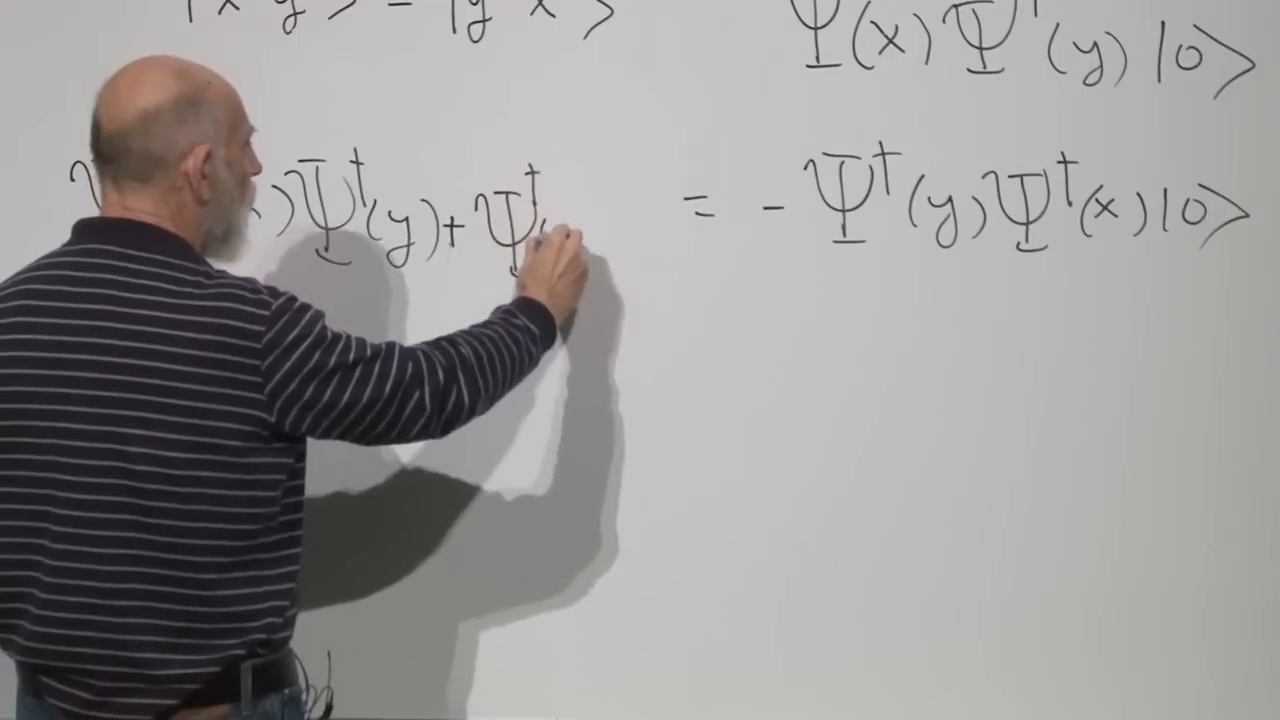
\includegraphics[width=0.94\linewidth]{lecture_10_figure_02.png}
\caption{フェルミオン的交換を実装する黒板上の関係式。生成演算子を入れ替えると二粒子状態の符号が反転する。}
\lectureframe{00:05:50}
\end{figure}

任意の二つの演算子\(A\)と\(B\)に対し、反交換子を
\begin{equation}
\{A,B\}:=AB+BA.
\end{equation}
で定義する。したがって交換規則は
\begin{equation}
\{\psi^\dagger(x),\psi^\dagger(y)\}=0.
\label{eq:l10-creation-anticommutator}
\end{equation}
である。対応するフェルミオン的場の代数は、ボソン的交换子を反交換子に置き換える。この語の二つの用法を区別して保たなければならない：場の演算子はフェルミ統計のために反交換し、一方、行列は後に相対論的分散関係における交差項を相殺するために反交換することになる。

ここで式~\eqref{eq:l10-creation-anticommutator}において\(y=x\)と置く。二つの積は同じものになる。
\begin{align}
0
&=\{\psi^\dagger(x),\psi^\dagger(x)\}\\
&=2\,\psi^\dagger(x)\psi^\dagger(x).
\end{align}
したがって
\begin{equation}
\bigl(\psi^\dagger(x)\bigr)^2=0.
\label{eq:l10-exclusion}
\end{equation}
同じ一粒子状態に二つの同種のフェルミオンを生成しようとすると、零ベクトルが得られる。これが演算子で表した排他原理である。

\begin{figure}[htbp]
\centering
\includegraphics[width=0.94\linewidth]{lecture_10_figure_03.png}
\caption{黒板上での等状態への特殊化。繰り返された生成演算子の積が二度現れるため、消えなければならない。}
\lectureframe{00:08:04}
\end{figure}

\begin{figure}[htbp]
\centering
\begin{adjustbox}{max width=\linewidth}
\begin{tikzpicture}[node distance=1.25cm,>=Latex]
\node[draw,rounded corners,align=center,inner sep=7pt] (a)
  {$\{\psi^\dagger(x),\psi^\dagger(x)\}=0$};
\node[draw,rounded corners,align=center,inner sep=7pt,right=of a] (b)
  {$2(\psi^\dagger(x))^2=0$};
\node[draw,rounded corners,align=center,inner sep=7pt,right=of b] (c)
  {$(\psi^\dagger(x))^2=0$};
\draw[->,thick] (a) -- (b);
\draw[->,thick] (b) -- (c);
\end{tikzpicture}
\end{adjustbox}
\caption{部分的に消された中間の黒板の作業なしに再構成された排他の議論。}
\end{figure}

\section{なぜフェルミオンでは充填と空が対称なのか}

ボソン的演算子とフェルミオン的演算子の間には、排他よりも微妙で、後に本質的となる第二の違いがある。単一のボソンモードに対して、
\begin{equation}
[a,a^\dagger]=1,
\qquad
n=0,1,2,\ldots.
\end{equation}
\(a\)と\(a^\dagger\)を入れ替えると交換子の符号が変わる。たとえ演算子が単に\(A\)と\(B\)と呼ばれていたとしても、代数はどちらの順序が占有数を上げ、どちらが下げるかを教えてくれる。

ボソン的占有はしごにも向きがある。消滅演算子はやがて\(\lvert0\rangle\)に達して零を与えるが、生成演算子は無限に続くことができる：
\begin{align}
a\lvert0\rangle&=0,\\
a^\dagger\lvert n\rangle&\propto\lvert n+1\rangle,
\qquad n=0,1,2,\ldots.
\end{align}
このはしごを上下逆にしても同じスペクトルは再現されない。底はあるが頂上はない。

単一のフェルミオンモードに対して、
\begin{equation}
\{a,a^\dagger\}=1,
\qquad
a^2=(a^\dagger)^2=0,
\qquad
n=0,1.
\label{eq:l10-fermion-mode}
\end{equation}
生成演算子は空の状態を充填された状態へと移し、そこで止まる：
\begin{equation}
a^\dagger\lvert0\rangle=\lvert1\rangle,
\qquad
a^\dagger\lvert1\rangle=0.
\end{equation}
消滅演算子は逆を行う：
\begin{equation}
a\lvert1\rangle=\lvert0\rangle,
\qquad
a\lvert0\rangle=0.
\end{equation}
状態は二つしかないので、図は充填と空、および\(a\)と\(a^\dagger\)の交換の下で対称である。演算子は依然として異なる物理的意味を持つが、その代数はもはや一方を生成、他方を消滅として選び出さない。この形式的対称性が粒子-正孔再解釈の種である。

\begin{classroomqa}
\lecturetimestamp{00:13:54}
\audiencequestion{もし\((a^\dagger)^2=0\)ならば、それは矛盾なのか、それとも\(a^\dagger=0\)を意味するのか？}
\lecturerresponse{どちらでもない。非零の演算子は零の二乗を持ちうる。ここで\(a^\dagger\)は\(\lvert0\rangle\)を\(\lvert1\rangle\)へと移すが、\(\lvert1\rangle\)の上には許された状態が存在しないので、二度作用させると零を与える。同じ推論により\(a^2=0\)が得られる。}
\end{classroomqa}

この「埋まった状態と空の状態」の対称性は、取っておこう。負エネルギーの電子が取り除かれると、消滅演算子は陽電子の生成演算子として読み替えられる。この移行は恣意的な記法の変更ではなく、ここで確立した二状態フェルミオン代数をまさに用いるものである。

\section{一次元ディラック構成}

ここで、一次元空間中の一粒子に戻ろう。最も単純な一階の相対論的波動方程式は
\begin{equation}
i\partial_t\psi=-\,i\partial_x\psi.
\label{eq:l10-right-mover}
\end{equation}
であり、\(P=-i\partial_x\)を用いれば
\begin{equation}
H=P.
\end{equation}
となる。運動量固有状態は\(E=p\)を持ち、その群速度は
\begin{equation}
v_g=\frac{dE}{dp}=1.
\end{equation}
である。正または負の運動量、したがって正または負のエネルギーは、依然として剛体的に右へ進む波を与える。\(p\)の符号は位相パターンを変えるのであって、伝播方向を変えるのではない。

質量を持つ粒子はどちらの方向にも動けなければならない。
\begin{equation}
H\psi_1=P\psi_1,
\qquad
H\psi_2=-P\psi_2.
\label{eq:l10-two-directions}
\end{equation}
を満たす第二の成分を導入しよう。第一の成分は右へ動き、第二の成分は左へ動く。それらを列にまとめ、
\begin{equation}
\Psi=
\begin{pmatrix}
\psi_1\\
\psi_2
\end{pmatrix},
\end{equation}
とし、
\begin{equation}
\alpha=
\begin{pmatrix}
1&0\\
0&-1
\end{pmatrix}.
\end{equation}
を定義する。両方の方程式は
\begin{equation}
H\Psi=\alpha P\Psi.
\label{eq:l10-massless-one-d}
\end{equation}
となる。両方向を含める代償は、新たな二値の内部自由度である。

方向だけでは質量は生じない。第二の行列
\begin{equation}
\beta=
\begin{pmatrix}
0&1\\
1&0
\end{pmatrix},
\end{equation}
を導入し、
\begin{equation}
H=\alpha P+\beta m.
\label{eq:l10-massive-one-d}
\end{equation}
を試みる。行列は
\begin{equation}
\alpha^2=\beta^2=\mathbb{1},
\qquad
\{\alpha,\beta\}=0.
\label{eq:l10-one-d-algebra}
\end{equation}
を満たす。ハミルトニアンを二乗すると
\begin{align}
H^2
&=(\alpha P+\beta m)^2\\
&=\alpha^2P^2+\beta^2m^2
  +(\alpha\beta+\beta\alpha)Pm\\
&=P^2+m^2.
\label{eq:l10-one-d-dispersion}
\end{align}
となる。式~\eqref{eq:l10-one-d-algebra}の反交換子が、\(P\)と\(m\)の両方に線形な不要項を消去する。

非対角行列\(\beta\)は二つの方向成分を結合する。質量項は右進振幅と左進振幅を絶えず混合していると描くと有用である。この描像を、粒子が微視的な軌道上を行き来して跳ね返るという文字通りのものにしてはならないが、なぜ質量を持つ波束が光より遅い平均速度を持ち得て静止系を持ち得るのか、一方、孤立した質量ゼロのカイラル成分はそうでないのかを捉えている。

\begin{classroomqa}
\lecturetimestamp{00:23:37}
\audiencequestion{両方の方向成分を導入することに、より深い物理的解釈はあるのか。}
\lecturerresponse{あるが、それは三次元でより明確に現れる。この段階では、それらは反対向きの伝播を記述し、非対角な質量結合を許すために必要な二つの成分にすぎない。それらの後の解釈は、利き手、すなわちカイラリティである。}
\end{classroomqa}

\section{三次元はパウリ行列を強制する}

三次元空間では運動量はベクトルである。したがって、運動量に線形で回転スカラーなハミルトニアンは、別のベクトル、今度は成分が行列であるベクトルを示唆する：
\begin{equation}
H=\boldsymbol{\alpha}\cdot\mathbf P
=\alpha_xP_x+\alpha_yP_y+\alpha_zP_z.
\label{eq:l10-three-d-ansatz}
\end{equation}

\begin{figure}[htbp]
\centering
\includegraphics[width=0.94\linewidth]{lecture_10_figure_04.png}
\caption{三次元の質量ゼロの仮定\(H=\boldsymbol{\alpha}\cdot\mathbf P\)は、一つの行列が三つの行列のベクトルになる点にある。}
\lectureframe{00:26:00}
\end{figure}

再び質量ゼロの場合から始めよう。
\begin{equation}
H^2=\mathbf P^2=P_x^2+P_y^2+P_z^2.
\end{equation}
を要求する。式~\eqref{eq:l10-three-d-ansatz}の二乗を展開すると、
\begin{align}
H^2
&=\alpha_x^2P_x^2+\alpha_y^2P_y^2\\
&\quad+\alpha_z^2P_z^2\\
&\quad+\{\alpha_x,\alpha_y\}P_xP_y\\
&\quad+\{\alpha_x,\alpha_z\}P_xP_z\\
&\quad+\{\alpha_y,\alpha_z\}P_yP_z.
\end{align}
対角項は
\begin{equation}
\alpha_x^2=\alpha_y^2=\alpha_z^2=\mathbb{1},
\end{equation}
ならば正しく、すべての交差項は
\begin{equation}
\{\alpha_i,\alpha_j\}=0,
\qquad i\ne j.
\label{eq:l10-alpha-anticommutation}
\end{equation}
ならば消える。

三つのおなじみの\(2\times2\)行列がまさにこれを行う：
\begin{equation}
\sigma_x=
\begin{pmatrix}
0&1\\
1&0
\end{pmatrix},
\quad
\sigma_y=
\begin{pmatrix}
0&-i\\
i&0
\end{pmatrix},
\quad
\sigma_z=
\begin{pmatrix}
1&0\\
0&-1
\end{pmatrix}.
\label{eq:l10-pauli-matrices}
\end{equation}
したがって一つの解は
\begin{equation}
\alpha_i=\sigma_i,
\qquad
H=\boldsymbol{\sigma}\cdot\mathbf P.
\label{eq:l10-weyl-hamiltonian}
\end{equation}
である。

\begin{figure}[htbp]
\centering
\includegraphics[width=0.94\linewidth]{lecture_10_figure_05.png}
\caption{コンパクトな質量ゼロのハミルトニアン\(H=\boldsymbol{\sigma}\cdot\mathbf P\)、その上に\(\alpha_z=\sigma_z\)が依然として見えている。}
\lectureframe{00:28:16}
\end{figure}

運動量固有状態に対して、
\begin{equation}
\boldsymbol{\sigma}\cdot\mathbf p
=
|\mathbf p|\,\boldsymbol{\sigma}\cdot\widehat{\mathbf p}.
\end{equation}
演算子\(\boldsymbol{\sigma}\cdot\widehat{\mathbf p}\)は固有値\(+1\)と\(-1\)を持つので、
\begin{equation}
E=\pm|\mathbf p|.
\end{equation}
この二成分理論では、正エネルギーはパウリ自由度が運動量と整列し、負エネルギーはそれが反整列している。この整列は固定されており、固定されたエネルギー符号に対して独立に調整できるスピン方向ではない。

\begin{classroomqa}
\lecturetimestamp{00:30:10}
\audiencequestion{スピンはディラック方程式から自然に現れるのか、それとも電子が既に磁気モーメントを持つことが知られているために挿入されたのか。}
\lecturerresponse{ここで「自然に現れる」とは「帰結として現れる」という意味であり、「消える」という意味ではない。出発点の要求は、二乗が\(\mathbf P^2\)となる、運動量に線形なハミルトニアンであった。通常の数は要求される代数を満たせないが、パウリ行列は満たすことができる。したがってそれらの二成分構造は、線形化そのものとともに現れる。これはすべての粒子がスピンを持たねばならないことを証明するものではない。このディラック型方程式で記述される粒子は、対応するスピノル自由度を担う、と言っているのである。}
\end{classroomqa}

これはこの構成の中心的な教訓の一つである。行列は、相対論的方程式が見つかった後に付け加えられる装飾的なラベルではない。相対論的分散関係の局所的な平方根を取ろうとする試みが、それらを生み出すのである。

\section{なぜ質量は四成分を必要とするのか}

\(2\times2\)理論を拡大することなく一次元の質量構成を繰り返そうと試みる：
\begin{equation}
H=\boldsymbol{\sigma}\cdot\mathbf P+\beta m.
\label{eq:l10-failed-mass}
\end{equation}
\(\beta^2=\mathbb{1}\)を仮定する。その二乗には望ましい項\(\mathbf P^2+m^2\)が含まれるが、同時に
\begin{equation}
m\sum_i\{\sigma_i,\beta\}P_i.
\end{equation}
も含まれる。この項を除去するには、一つの行列\(\beta\)が
\begin{equation}
\{\sigma_x,\beta\}
=
\{\sigma_y,\beta\}
=
\{\sigma_z,\beta\}
=0.
\label{eq:l10-impossible-beta}
\end{equation}
を満たさなければならない。そのような\(2\times2\)行列は存在しない。単位行列は三つのパウリ行列すべてと可換であり、トレースが零の任意の\(2\times2\)行列はパウリ行列の線形結合である。そのような結合は、それに平行な成分と反可換にならない。\(2\times2\)代数には、要求される種類の第四の独立な行列が存在しない。

救済策はスピノルを拡大することである。二乗が単位行列となる四つの相互に反可換な行列は、\(4\times4\)複素表現において初めて現れる。この行列の大きさは、時空が四次元であるから選ばれたのではない。要求される代数を実現できる最小の行列空間だからである。

多くの等価な表現が存在する。スピノル基底のユニタリ変換は、いかなる物理的予言も変えることなく、すべての行列の成分を変える。重要なのは、関係式の抽象的な集合
\begin{equation}
\{\alpha_i,\alpha_j\}=2\delta_{ij}\mathbb{1},
\qquad
\{\alpha_i,\beta\}=0,
\qquad
\beta^2=\mathbb{1}.
\label{eq:l10-dirac-algebra}
\end{equation}
である。

\begin{classroomqa}
\lecturetimestamp{00:37:38}
\audiencequestion{\(\beta\)を時間成分\(\alpha_t\)と見なせるか？}
\lecturerresponse{直接にはできない。三つの\(\alpha_i\)は、一つのローレンツベクトルの四つの成分として\(\beta\)と結合しない。共変的表記では、代わりに\(\beta=\gamma^0\)および\(\alpha_i=\gamma^0\gamma^i\)を定義する。四つの\(\gamma^\mu\)行列は時空のクリフォード代数を満たす。}
\end{classroomqa}

便利なブロック表現は
\begin{equation}
\alpha_i=
\begin{pmatrix}
\sigma_i&0\\
0&-\sigma_i
\end{pmatrix},
\qquad
\beta=
\begin{pmatrix}
0&I_2\\
I_2&0
\end{pmatrix}.
\label{eq:l10-block-representation}
\end{equation}
である。対角ブロック内のパウリ行列は、異なる\(\alpha_i\)が反可換であることを保証する。\(\beta\)内の非対角な単位行列ブロックは、\(\beta\)がすべての\(\alpha_i\)と反可換であることを保証する。

\begin{figure}[htbp]
\centering
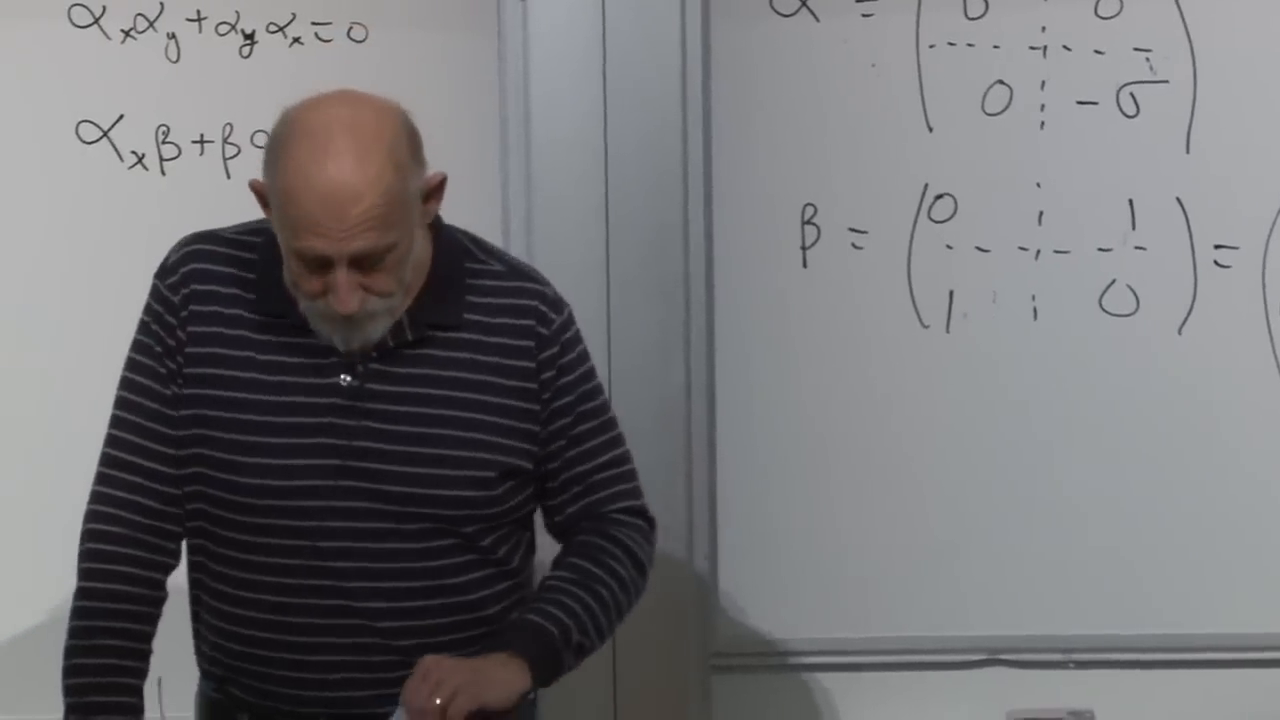
\includegraphics[width=0.94\linewidth]{lecture_10_figure_06.png}
\caption{黒板の\(4\times4\)ブロック表現。上の式は要求される反可換子を記録している。完全な行列は式~\eqref{eq:l10-block-representation}に組版されている。}
\lectureframe{00:41:10}
\end{figure}

質量をもつハミルトニアンは今や
\begin{equation}
H=\boldsymbol{\alpha}\cdot\mathbf P+\beta m
=
\begin{pmatrix}
\boldsymbol{\sigma}\cdot\mathbf P&mI_2\\
mI_2&-\boldsymbol{\sigma}\cdot\mathbf P
\end{pmatrix}.
\label{eq:l10-massive-dirac}
\end{equation}
である。式~\eqref{eq:l10-dirac-algebra}を用いると、
\begin{equation}
H^2=\mathbf P^2+m^2.
\end{equation}
したがって四次元構造は任意の装飾ではない。三次元運動量と質量項の両方を許しつつ方程式を一階に保つ最小の構造なのである。

\section{カイラリティと余分な成分の意味}

この拡大はどのような物理的区別を加えたのか？ まず質量のない上ブロック
\begin{equation}
H_R=\boldsymbol{\sigma}\cdot\mathbf P,
\end{equation}
と、質量のない下ブロック
\begin{equation}
H_L=-\boldsymbol{\sigma}\cdot\mathbf P.
\end{equation}
から始める。正エネルギーの状態について、第一のものはスピンが運動量と整列し、第二のものはスピンが反整列している。これらは反対のヘリシティである。質量のない理論では、ヘリシティは固有ローレンツ変換の下で不変である。なぜなら、いかなる観測者も光速的な粒子を追い越し、そのスピンを変えずに運動量を反転させることはできないからである。したがって二つのブロックは反対のカイラルセクターを記述する。

\begin{classroomqa}
\lecturetimestamp{00:41:28}
\audiencequestion{一次元では質量を導入するために余分な二値的自由度が必要であった。三次元における対応する物理的区別は何か？}
\lecturerresponse{それはスピノルの巻き性である。二つの\(2\times2\)ブロックはスピンと運動量の間の反対の関係を担う。一方は右手型であり、他方は左手型である。\(4\times4\)理論は両方を含む。}
\end{classroomqa}

式~\eqref{eq:l10-massive-dirac}の質量項は非対角的である。それは上ブロックの振幅を下ブロックへ送り、その逆も同様である：
\begin{equation}
\beta m
\begin{pmatrix}
\Psi_R\\
\Psi_L
\end{pmatrix}
=
m
\begin{pmatrix}
\Psi_L\\
\Psi_R
\end{pmatrix}.
\end{equation}
したがって質量は反対のカイラリティ間の結合である。

\begin{classroomqa}
\lecturetimestamp{00:43:58}
\audiencequestion{質量のない粒子はカイラリティを変えられるか？}
\lecturerresponse{ここに示された自由な質量のないハミルトニアンでは変えられない。二つのブロックは分離しているので、右手型または左手型として始まった状態はそのままである。非対角な質量項こそが、\(m\ne0\)のときにそれらを混合するものである。}
\end{classroomqa}

この言葉遣いはブロック表現に対しては正確であるが、粒子が二つの矢印の間で機械的に反転するというイメージはあまり押し進めるべきではない。物理的な主張は波動方程式における行列の結合である。

\begin{classroomqa}
\lecturetimestamp{00:44:50}
\audiencequestion{これらの行列は四元数に組み込まれているのか？}
\lecturerresponse{パウリ行列は四元数単位と密接に関係している。行列\(-i\sigma_i\)は二乗すると\(-\mathbb{1}\)となり、向きの規約を除いて四元数のパターンで乗算される。完全なディラック行列はより大きなクリフォード代数を必要とし、四元数との関連は以下の議論には必要ない。}
\end{classroomqa}

\begin{classroomqa}
\lecturetimestamp{00:46:34}
\audiencequestion{スピンが角運動量であるなら、ここでそれに関連する別個のエネルギー項は存在するのか。}
\lecturerresponse{独立な自由粒子項は加えられていない。スピノル構造はすでに行列を通じて運動項のハミルトニアンに入っている。スピンを外部磁場に結合させれば追加の相互作用項が導入されるが、それは別の問題である。}
\end{classroomqa}

\section{アルファ行列は速度であり、スピンではない}

各\(\alpha_i\)は二つの\(+1\)固有値と二つの\(-1\)固有値をもつ。異なる成分は可換でないため、それらすべてを同時に鋭く測定することはできない。ある成分が何を表すかを同定するには、ハイゼンベルク方程式を用いる。陽に時間依存しない演算子\(L\)に対して、
\begin{equation}
\dot L=i[H,L].
\label{eq:l10-heisenberg}
\end{equation}
ここでは符号の規約はSchr\"odinger発展\(e^{-iHt}\)によって固定されている。

式~\eqref{eq:l10-heisenberg}を位置演算子\(x\)に適用する。行列はスピノル添字に作用し、位置と可換である。一方、\(P_x\)だけが\(x\)と可換でない：
\begin{align}
\dot x
&=i[\boldsymbol{\alpha}\cdot\mathbf P+\beta m,x]\\
&=i\alpha_x[P_x,x]\\
&=\alpha_x,
\label{eq:l10-velocity}
\end{align}
なぜなら\([P_x,x]=-i\)だからである。したがって\(\alpha_x\)は速度演算子の\(x\)成分であり、同様に、
\begin{equation}
\dot{\mathbf x}=\boldsymbol{\alpha}.
\end{equation}

\begin{classroomqa}
\lecturetimestamp{00:51:50}
\audiencequestion{速度成分の測定は本当に\(+1\)か\(-1\)しか与えないのか。}
\lecturerresponse{はい、単位\(c=1\)での瞬時演算子\(\alpha_i\)についてはそうである。一般の状態は固有状態である必要はないので、その期待値はそれらの値の間のどこにでもあり得る。滑らかに輸送される波束は、粒子が質量をもつとき、光速未満の平均速度をもつ。}
\end{classroomqa}

速度は保存されない：
\begin{equation}
\dot\alpha_x=i[H,\alpha_x]\ne0.
\end{equation}
\(\alpha_y\)、\(\alpha_z\)、\(\beta\)を含む項は\(\alpha_x\)と可換でない。したがって、正エネルギー成分と負エネルギー成分の両方を含む状態は、その位置に急速な振動的寄与を示す。これが\emph{ツィッターベヴェーグング}、文字通り震える運動である。

急速な振動に比べて長い時間で平均した後、期待される相対論的速度は
\begin{equation}
\overline{\mathbf v}=\frac{\mathbf p}{E},
\end{equation}
であり、遅い電子に対して\(\mathbf p/m\)に帰着する。

\begin{classroomqa}
\lecturetimestamp{00:54:40}
\audiencequestion{外力なしで自由電子が震えることはニュートンの法則に反しないのか。}
\lecturerresponse{反しない。並進不変性は運動量を保存するので、\(\dot{\mathbf P}=0\)である。ディラック速度演算子は単に\(\mathbf P/m\)ではなく、その急速な振動部分は運動量が固定されたままで変化し得る。時間平均された運動は期待される自由粒子の関係に従う。}
\end{classroomqa}

\begin{classroomqa}
\lecturetimestamp{00:55:22}
\audiencequestion{速度は常に\(c\)なのか。}
\lecturerresponse{一つの\(\alpha_i\)の瞬時測定は固有値\(\pm c\)をもつが、質量をもつ波束は一般に重ね合わせであり、光速未満の期待値をもつ。その平均群速度は\(\mathbf p/E\)である。}
\end{classroomqa}

\begin{classroomqa}
\lecturetimestamp{00:55:30}
\audiencequestion{振動は質量が速度を変化させるものとして描けるのか。}
\lecturerresponse{いいえ。質量は固定されたパラメータである。振動は非可換な速度演算子とハミルトニアン演算子から、あるいは同等にエネルギー部門間の干渉から生じるのであり、変動する質量からではない。}
\end{classroomqa}

\begin{classroomqa}
\lecturetimestamp{00:56:22}
\audiencequestion{瞬時測定が、平均運動が別の向きを指しているにもかかわらず、速度がある向きを指していると見出すことはあり得るか。}
\lecturerresponse{はい。成分演算子は二つの鋭い固有値をもつ一方、繰り返し測定または時間平均測定はより滑らかなドリフトを回復する。}
\end{classroomqa}

スピンという語も注意深く用いなければならない。\(\alpha_i\)は速度の成分、すなわち通常のベクトルとして変換する。この表現における真のスピン演算子は
\begin{equation}
\mathbf S=\frac12\boldsymbol{\Sigma},
\qquad
\Sigma_i=
\begin{pmatrix}
\sigma_i&0\\
0&\sigma_i
\end{pmatrix}.
\label{eq:l10-spin-operator}
\end{equation}
であり、\(\alpha_i\)とは下のブロックの符号だけが異なる。行列は密接に関係しているが、速度とスピンは同じオブザーバブルではない。

\section{負エネルギーと最低エネルギー真空}

負エネルギーの問題は、このような行列の仕組みの前にすでに存在している。一次元の右向き運動に戻ると、
\begin{equation}
H=P.
\end{equation}
\(p\)は実数直線全体を動くので、\(E=p\)には下界がない。

真空は単に粒子が存在しない状態を意味することはできない。それ以上エネルギーを奪えない状態でなければならない。もし空の状態が負エネルギーの粒子を加えることを許し、エネルギーを下げ、さらに別の粒子を加え、以下無限に続けられるならば、その空の状態は安定な真空ではない。

フェルミ統計が歴史的な解決策を与える。すべての負エネルギー状態に電子を1個ずつ置く。電子を追加するたびに全エネルギーは下がるが、排他律により各一粒子状態には電子を1個しか入れられない。すべての負エネルギー状態が埋まると、それ以上電子はこのセクターへ落ち込めない。ディラックはこの埋まった配置を真空と同定した。

同じ構成はボソンでは破綻する。任意個のボソンが1つの状態を占めうるので、負エネルギーのボソン的モードは際限なく粒子を吸収できてしまう。講義の冒頭で導入したフェルミオン的束縛 \(n=0,1\) こそが、この下降を止めるものである。

\begin{figure}[htbp]
\centering
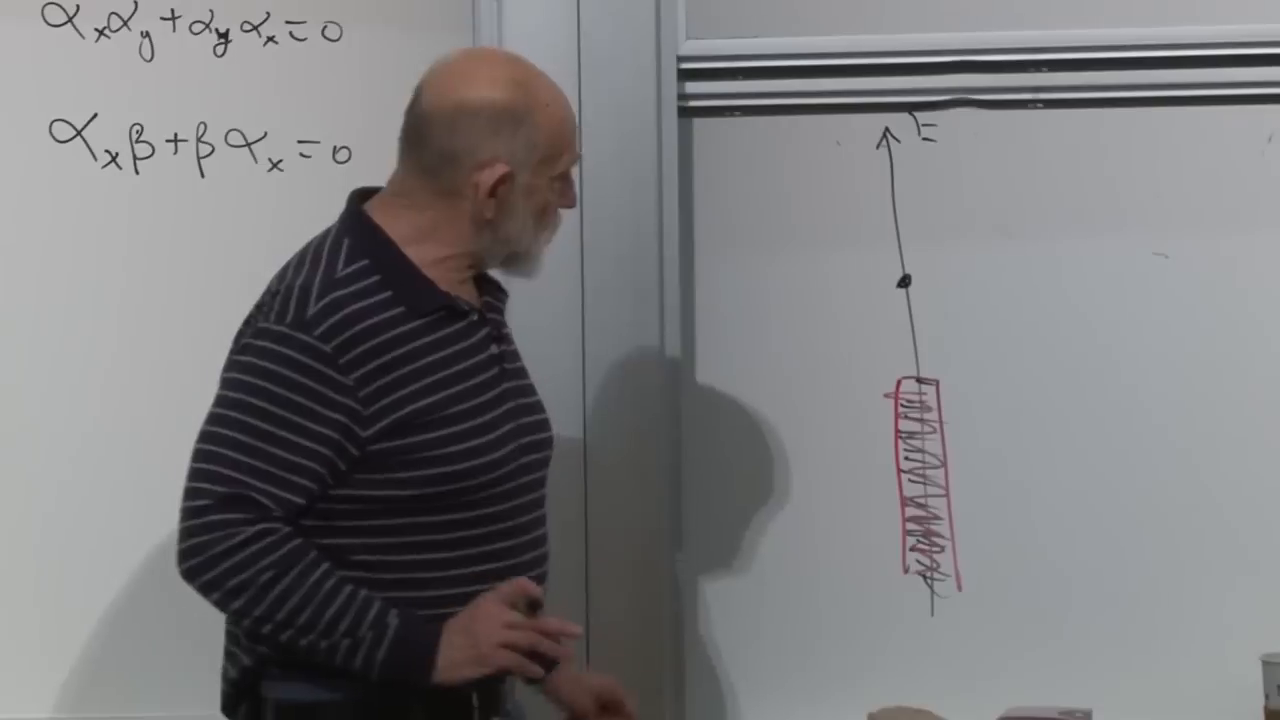
\includegraphics[width=0.94\linewidth]{lecture_10_figure_07.png}
\caption{黒板上の歴史的なディラックの海の描像：負エネルギー準位のはしごが分割線まで埋まり、その上に正エネルギー状態がある。}
\lectureframe{01:02:45}
\end{figure}

\begin{figure}[htbp]
\centering
\begin{adjustbox}{max width=\linewidth}
\begin{tikzpicture}[x=1.05cm,y=0.72cm,>=Latex]
\draw[->] (0,-4.8) -- (0,4.8) node[above] {$E$};
\draw[thick] (-2.9,0) -- (3.2,0) node[right] {$E=0$};
\foreach \y in {-4,-3.3,...,-0.5} {
  \draw (-2.3,\y) -- (2.3,\y);
  \foreach \x in {-1.8,-1.2,...,1.8} {
    \fill[blue!65!black] (\x,\y) circle (1.6pt);
  }
}
\foreach \y in {0.8,1.6,...,4.0} {
  \draw (-2.3,\y) -- (2.3,\y);
}
\draw[red,very thick] (0.6,-2.6) circle (5pt);
\draw[red,->,very thick] (0.6,-2.35) .. controls (1.4,-0.4) and (1.2,1.6) .. (1.5,2.4);
\fill[red] (1.5,2.4) circle (2.5pt);
\node[right,red] at (0.85,-2.6) {hole};
\node[right,red] at (1.7,2.4) {$e^-$};
\node[left] at (-2.5,-2.2) {filled negative-energy states};
\end{tikzpicture}
\end{adjustbox}
\caption{埋まった海の上の励起の明快な再構成：負エネルギーの電子を1個励起すると、正エネルギーの正孔が残る。}
\end{figure}

海の描像は、正しい演算子の再配列に対する歴史的な言葉である。その文字通りの無限の電荷とエネルギーを直接観測可能な量と誤解してはならない。現代的な再定式化は、物質的な電子が空間を満たすと想像する必要を取り除く。

\section{正孔は陽電子である}

すべての負エネルギー状態が占有されているとき、2種類の励起が可能である。海の上に正エネルギーの電子を加えてもよい。あるいは負エネルギーの電子を1個取り除いて正孔を残してもよい。

正孔は、失われた電子とは反対の電荷をもつ。電荷 \(-e\) を取り除くと電荷は \(+e\) だけ変化する。また正の励起エネルギーをもつ。取り除かれた電子が \(E_-<0\) であったなら、埋まった真空を基準に測ったエネルギーは次だけ変化する
\begin{equation}
E_{\mathrm{hole}}=-E_->0.
\end{equation}
正孔は正エネルギーで正電荷の励起、すなわち陽電子である。

光子は海の電子を正エネルギー状態へ励起できる。真空を基準にすると、最終状態は電子と陽電子を含む。時間順序図では、電子については電子数の流れを上向きに描き、陽電子の線は逆向きの矢印で描くのが慣例である。矢印はフェルミオン数または電荷の流れを追うものであり、古典的な小さな速度ベクトルではない。

\begin{classroomqa}
\lecturetimestamp{01:05:14}
\audiencequestion{この描像は電子と陽電子の数が等しいことを要求するか。}
\lecturerresponse{任意の状態については要求しない。真空から出発して中性の対を生成すれば1個ずつ得られるが、状態はすでに過剰な電子または過剰な陽電子を含んでいてもよい。電荷保存は反応を制約するが、すべての許された状態が等しい個数をもつことを要求するものではない。}
\end{classroomqa}

ディラックは当初、正孔が質量において電子と同一で、電荷およびその他の加法的量子数のみが反対の粒子になることを知らなかった。方程式と正孔の構成が、陽電子がよく知られた粒子目録に組み込まれる前に、その予言へと導いた。

\section{1つのフェルミオン場が電子と陽電子を含む}

場の演算子は、歴史的な描像を現代的な代数へと持ち込む。ここではスピノル指数、規格化因子、時間依存性をしばらく抑制する。一次元の場は模式的に次のように展開できる：
\begin{equation}
\psi(x)
\sim
\int_{-\infty}^{\infty}dp\,a(p)e^{ipx}.
\label{eq:l10-full-field-integral}
\end{equation}
右向きの分散関係 \(E=p\) に対して、正の \(p\) は正エネルギーを、負の \(p\) は負エネルギーを表す。積分を分割する：
\begin{equation}
\psi(x)
\sim
\int_0^\infty dp\,a(p)e^{ipx}
+
\int_{-\infty}^0 dp\,a(p)e^{ipx}.
\end{equation}
第二項で \(p=-q\) と置き、\(q>0\) として、満たされた負エネルギー電子の消滅を陽電子の生成として再解釈する：
\begin{equation}
b^\dagger(q):=a(-q).
\end{equation}
すると
\begin{equation}
\psi(x)
\sim
\int_0^\infty dp\,
\left[
a(p)e^{ipx}
+
b^\dagger(p)e^{-ipx}
\right].
\label{eq:l10-electron-positron-split}
\end{equation}
平面波の位相の正確な符号は時空の規約に依存する。不変な内容は、\(\psi\) が電子の消滅演算子と陽電子の生成演算子を含むということである。

\begin{figure}[htbp]
\centering
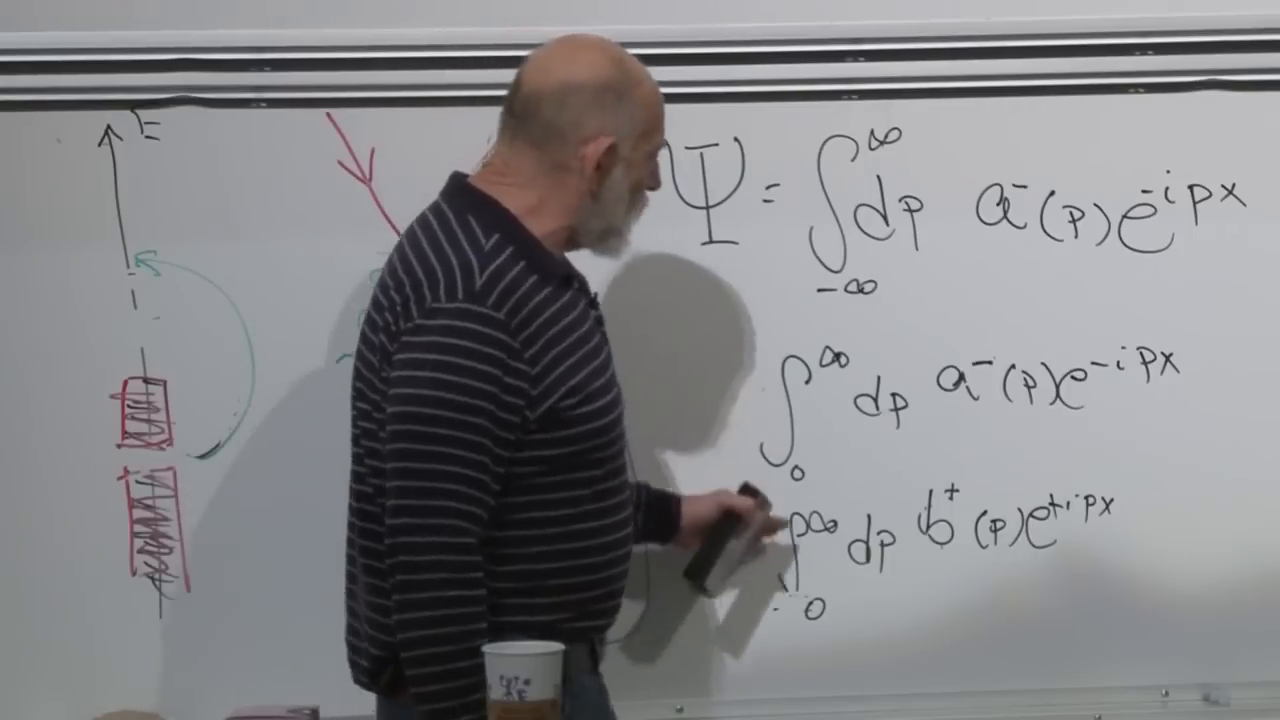
\includegraphics[width=0.94\linewidth]{lecture_10_figure_08.png}
\caption{場の積分を正エネルギーと負エネルギーのセクターに分割したもの。下の行は負エネルギーの電子演算子を陽電子生成演算子として付け替える。}
\lectureframe{01:11:35}
\end{figure}

ここで式~\eqref{eq:l10-fermion-mode}の埋まった-空の対称性が効いてくる。フェルミオンでは、演算子代数はその反交換構造を変えずにこの付け替えを許す。

電磁相互作用の模式的な形は
\begin{equation}
H_{\mathrm{int}}
\sim
\int dx\,\psi^\dagger(x)\psi(x)A(x),
\label{eq:l10-qed-schematic}
\end{equation}
である。ここで \(A\) は光子場を表す。各フェルミオン場は電子と陽電子の成分を含むため、単一の局所演算子がいくつかのチャネルを含む：
\begin{align}
e^-&\longrightarrow e^-+\gamma,\\
e^-+e^+&\longrightarrow\gamma,\\
\gamma&\longrightarrow e^-+e^+,
\end{align}
およびそれらの逆過程と交差過程である。どのチャネルが特定の環境で運動学的に可能かは、エネルギー・運動量保存が決める。例えば、真空中の孤立した実光子は、反跳を吸収する別の参加者がいなければ対を生成できない。局所頂点が相互作用に存在していてもである。

\begin{figure}[htbp]
\centering
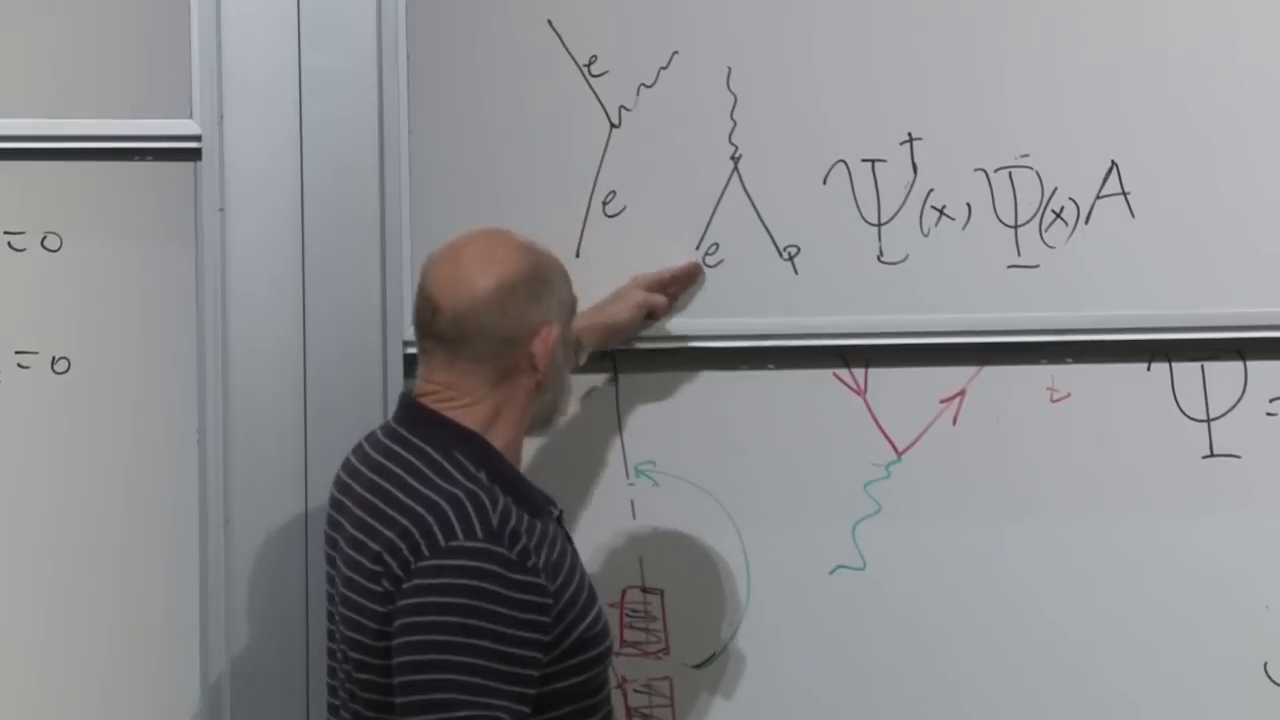
\includegraphics[width=0.94\linewidth]{lecture_10_figure_09.png}
\caption{黒板は電子放出、対消滅、および模式的な相互作用 \(\psi^\dagger\psi A\) を並置している。同じ場の演算子から異なる選択をすることが、異なるチャネルを生み出す。}
\lectureframe{01:13:30}
\end{figure}

したがって、1つのコンパクトな場の積が、多くの見かけ上異なる反応を組織化する。ファインマンは後に振幅を評価するための体系的な図式規則を与えたが、演算子構造の多くはすでにここに見えている。

\section{現代の真空の言語とフェルミ海のアナロジー}

\begin{classroomqa}
\lecturetimestamp{01:14:20}
\audiencequestion{現代の物理学者は、真空を文字通りのディラックの海として扱うことなく、これをどのように記述するのか。}
\lecturerresponse{彼らは演算子の再解釈を直接行う。負エネルギーの電子の消滅は、正エネルギーの陽電子の生成と改名され、真空はすべての電子と陽電子の消滅演算子によって消滅させられる状態として定義される。得られる定式化は粒子と反粒子の間で対称であり、物質的な海を必要としない。}
\end{classroomqa}

歴史的な海は、その論理が凝縮系に近い類似をもつため、依然として有用である。結晶では、固定された数の電子が、フェルミ準位までの利用可能な最低の一粒子状態を満たす。満たされた基底状態は空ではない。1つの電子をその準位より上に励起すると、その下に非占有状態が残る。満たされた背景に対して、正孔は正の励起エネルギーを持ち、正の電荷キャリアとして振る舞うことができる。

重要な違いがある。固体中の正孔は媒質中に存在し、その有効質量と電荷応答はバンド構造に依存する。陽電子は相対論的量子場における素粒子の反粒子である。それでもなお、共通の粒子-正孔代数がこのアナロジーを強力にする。

\begin{classroomqa}
\lecturetimestamp{01:17:14}
\audiencequestion{ボソンに対するKlein--Gordon理論も、負エネルギー状態への同じカスケードに陥るのだろうか。}
\lecturerresponse{いや、そうではない。適切に量子化された複素Klein--Gordon場は、ボソンの海を埋めることなく、正エネルギーの粒子と反粒子へと組織化される。その二階の方程式と正準構造はDiracハミルトニアンの構成とは異なるため、歴史的なフェルミオン的海の議論がそのまま移されるわけではない。}
\end{classroomqa}

\begin{classroomqa}
\lecturetimestamp{01:17:30}
\audiencequestion{ボソンのスピン1はどこから来るのか。}
\lecturerresponse{ここで用いられたパウリ行列の線形化からではない。スピン1の場はそれ自身のローレンツ変換則と場の方程式をもつ。現在の導出はディラックフェルミオンのスピノル構造を説明するものであり、可能なすべての粒子スピンを説明するものではない。}
\end{classroomqa}

\begin{classroomqa}
\lecturetimestamp{01:17:46}
\audiencequestion{なぜフェルミ統計が負エネルギー解に不可欠だったのか。}
\lecturerresponse{排他律が各状態を1つの電子に制限するからである。すべての負エネルギー状態が占有されると、それ以上電子はそれらに落ち込めない。ボソンの占有にはそのような上限がないため、文字通りの負エネルギーのボソンの海には依然として底がない。}
\end{classroomqa}

\begin{classroomqa}
\lecturetimestamp{01:20:02}
\audiencequestion{電子対陽電子は、電荷のように単に別の二値的自由度なのか。}
\lecturerresponse{状態の数え方としては、質量をもつディラック場は2つの電子スピン状態と2つの陽電子スピン状態をもつので、2つの二値ラベルは有用な記憶法である。しかし粒子対反粒子は、1つの電子の独立に回転できる内部量子ビットではない。すべての電子は電荷 \(-e\) をもち、すべての陽電子は \(+e\) をもち、その区別は量子化後の正周波数と負周波数のセクターから現れる。}
\end{classroomqa}

無限の海は最後に1つの疑問を提起する。

\begin{classroomqa}
\lecturetimestamp{01:20:54}
\audiencequestion{無限のディラックの海は無限の宇宙定数を生み出すのだろうか。}
\lecturerresponse{それは真空エネルギーの問題を露呈させる。ボソンの零点モードは\(+\tfrac12\hbar\omega\)に寄与するが、フェルミオン的モードは逆の符号で寄与する。スペクトルが一致する場合には形式的な相殺が可能であるが、電子と光子のスペクトルは一致せず、莫大な残差が予想される。重力がなければ、エネルギーの差のみが重要であるため、ハミルトニアンの定数シフトは差し引くことができる。重力があれば、絶対的な真空エネルギーが重力に寄与するため、その差し引きは単なる帳尻合わせではなく物理的な問題となる。}
\end{classroomqa}

最後に戻るのは質量の意味についてである。

\begin{classroomqa}
\lecturetimestamp{01:22:56}
\audiencequestion{質量が左手系成分と右手系成分をどのように関係づけるかについて、さらに言えることはあるだろうか。}
\lecturerresponse{正確な記述はすでにハミルトニアンの中にある。非対角項\(m\beta\)が一方のカイラルブロックを他方へ写すのである。微視的な反転についてこれ以上に力学的な描像を与えることは任意であり、必然的に不完全である。}
\end{classroomqa}
\end{document}
